\chapter{AC electricity}

While \textit{direct current} (DC) refers to the flow of electrical charge carriers in a continuous direction, \textit{alternating current} (or \textit{AC}) refers to a periodic reversal of charge flow direction\footnote{It is also acceptable to refer to electrical voltages and/or currents that vary periodically over time even if their directions never alternate, as AC \textit{superimposed} on DC.}.  As a mode of transferring electrical power, AC is tremendously useful because it allows us to use \textit{transformers} to easily and efficiently step voltage up or down at will.  If an electro-physical sensor senses a physical quantity that oscillates, the electric signal it produces will oscillate (AC) as well.  For both these reasons, an instrument technician needs to be aware of how AC circuits work, and how to understand them mathematically.  \index{Direct current}  \index{Alternating current}  \index{DC}  \index{AC}






%\filbreak
%\section{Basic concepts}

% ADD: text, illustrations, photos, etc.








%\filbreak
%\section{Power sources}

% ADD: text, illustrations, photos, etc.






%\filbreak
%\section{Oscilloscopes}

% ADD: text, illustrations, photos, etc.








\filbreak
\section{RMS quantities}

It is often useful to express the amplitude of an alternating quantity such as voltage or current in terms that are equivalent to direct current (DC).  Doing so provides an ``apples-to-apples'' comparison between AC and DC quantities that makes comparative circuit analysis much easier.

The most popular standard of equivalence is based on \textit{work} and \textit{power}, and we call this the \textit{root-mean-square} value of an AC waveform, or RMS for short.  For example, an AC voltage of 120 volts ``RMS'' means that this AC voltage is capable of delivering the exact same amount of power (in Watts) at an electrical load as a 120 volt DC source powering the exact same load.  \index{RMS quantities}  \index{Root-mean-square (RMS) quantities}

The problem is exactly how to calculate this ``RMS'' value if all we know about the AC waveform is its peak value.  If we compare a sine wave and a DC ``wave'' side by side, it is clear that the sine wave must peak at a greater value than the constant DC level in order to be equivalent in terms of doing the same \textit{work} in the same amount of time:

$$\includegraphics{rms_01.eps}$$

At first, it might seem like the correct approach would be to use calculus to integrate (determine the area enclosed by) the sine wave over one-half of a cycle: from 0 to $\pi$ radians.  This is close, but not fully correct.  The ability of an electrical voltage to dissipate power at a resistor is not directly proportional to the magnitude of that voltage, but rather proportional to the \textit{square} of the magnitude of that voltage!  In mathematical terms, resistive power dissipation is predicted by the following equation:

$$P = {V^2 \over R}$$

If we double the amount of voltage applied to a resistor, the power increases four-fold.  If we triple the voltage, the power goes up by a factor of nine.  If we are to calculate the ``RMS'' equivalent value of a sine wave, we must take this nonlinearity into consideration.

\filbreak

First let us begin with a mathematical equivalence between the DC and AC cases.  For DC, the amount of \textit{work} done is equal to the constant power of that circuit multiplied by time.  The unit of measurement for power is the \textit{Watt}, which is defined as 1 Joule of work per second.  So, multiplying the steady power rate in a DC circuit by the time we keep it powered will result in an answer of joules (total energy dissipated by the resistor):

$$\hbox{Work} = \left({V^2 \over R} \right)t$$

Showing this equivalence by dimensional analysis:

$$[\hbox{Joules}] = \left([\hbox{Joules}] \over [\hbox{s}]\right) [\hbox{s}]$$

We cannot calculate the work done by the AC voltage source quite so easily, because the power dissipation varies over time as the instantaneous voltage rises and falls.  Work is still the product of power and time, but we cannot simply multiply one by the other because the voltage in this case is a \textit{function} of time ($V(t)$).  Instead, we must use integration to calculate the product of power and time, and sum those work quantities into a total work value.  

Since we know the voltage provided by the AC source takes the form of a sine wave ($V(t) = \sin t$ if we assume a sine wave with a peak value of 1 volt), we may write the formula for instantaneous AC power as follows:

$$\hbox{Power} = {\left(V(t)\right)^2 \over R} = {\sin^2 t \over R}$$

To calculate the work done by this sinusoidal voltage on the resistor, we will integrate this instantaneous power with respect to time, between the intervals of $t=0$ and $t=\pi$ (one half-cycle of the sine wave):  \index{Integration, applied to RMS waveform value}

$$\hbox{Work} = \int_0^\pi {{\sin^2 t} \over R} \> dt$$

In order to solve for the amount of DC voltage equivalent (from the perspective of resistive power dissipation) to a one-volt AC sine wave, we will set the DC work and AC work equations equal to each other, making sure the DC side of the equation has $\pi$ for the amount of time (being the same time interval as the AC side):

$$\left({V^2 \over R} \right) \pi = \int_0^\pi {{\sin^2 t} \over R} \> dt$$

Our goal is to solve for $V$ on the left-hand side of this equation.

\filbreak

First, we know that $R$ is a constant value, and so we may move it out of the integrand:

$$\left({V^2 \over R} \right) \pi = {1 \over R} \int_0^\pi \sin^2 t \> dt$$

Multiplying both sides of the equation by $R$ eliminates it completely.  This should make intuitive sense, as our RMS equivalent value for an AC voltage is defined strictly by the ability to produce the same amount of power as the same value of DC voltage for \textit{any} resistance value.  Therefore the actual value of resistance ($R$) should not matter, and it should come as no surprise that it cancels:

$$V^2 \pi = \int_0^\pi \sin^2 t \> dt$$

Now, we may simplify the integrand by substituting the half-angle equivalence for the $\sin^2 t$ function

$$V^2 \pi = \int_0^\pi {{1 - \cos 2t} \over 2} \> dt$$

Factoring one-half out of the integrand and moving it outside (because it's a constant):

$$V^2 \pi = {1 \over 2}\int_0^\pi 1 - \cos 2t \> dt$$

We may write this as the difference between two integrals, treating each term in the integrand as its own integration problem:

$$V^2 \pi = {1 \over 2} \left( \int_0^\pi 1 \> dt - \int_0^\pi \cos 2t \> dt \right)$$

The second integral may be solved simply by using substitution, with $u = 2t$, $du = 2 \> dt$, and $dt = {du \over 2}$:

$$V^2 \pi = {1 \over 2} \left( \int_0^\pi 1 \> dt - \int_0^\pi {\cos u \over 2} \> du \right)$$

Moving the one-half outside the second integrand:

$$V^2 \pi = {1 \over 2} \left( \int_0^\pi 1 \> dt - {1 \over 2}\int_0^\pi \cos u \> du \right)$$

\filbreak

Finally we are at a point where we may perform the integrations:

$$V^2 \pi = {1 \over 2} \left( \int_0^\pi 1 \> dt - {1 \over 2}\int_0^\pi \cos u \> du \right)$$

$$V^2 \pi = {1 \over 2} \left( \left[ t \right]_0^\pi - {1 \over 2}\left[\sin 2t \right]_0^\pi \right)$$

$$V^2 \pi = {1 \over 2} \left( [\pi - 0] - {1 \over 2}[\sin 2\pi - \sin 0] \right)$$

$$V^2 \pi = {1 \over 2} \left( [\pi - 0] - {1 \over 2}[0 - 0] \right)$$

$$V^2 \pi = {1 \over 2} (\pi - 0)$$

$$V^2 \pi = {1 \over 2}\pi$$

We can see that $\pi$ cancels out of both sides:

$$V^2 = {1 \over 2}$$

Taking the square root of both sides, we arrive at our final answer for the equivalent DC voltage value:

$$V = {1 \over \sqrt{2}}$$

So, for a sinusoidal voltage with a peak value of 1 volt, the DC equivalent or ``RMS'' voltage value would be ${1 \over \sqrt{2}}$ volts, or approximately 0.707 volts.  In other words, a sinusoidal voltage of 1 volt peak will produce just as much power dissipation at a resistor as a steady DC voltage of 0.7071 volts applied to that same resistor.  Therefore, this 1 volt peak sine wave may be properly called a 0.7071 volt RMS sine wave, or a 0.7071 volt ``DC equivalent'' sine wave.

This factor for sinusoidal voltages is quite useful in electrical power system calculations, where the wave-shape of the voltage is nearly always sinusoidal (or very close).  In your home, for example, the voltage available at any wall receptacle is 120 volts RMS, which translates to 169.7 volts peak.

Electricians and electronics technicians often memorize the $1 \over \sqrt{2}$ conversion factor without realizing it only applies to \textit{sinusoidal} voltage and current waveforms.  If we are dealing with a non-sinusoidal wave-shape, the conversion factor between peak and RMS \textit{will} be different!  The mathematical procedure for obtaining the conversion factor will be identical, though: integrate the wave-shape's function (squared) over an interval sufficiently long to capture the essence of the shape, and set that equal to $V^2$ times that same interval span.







\filbreak
\section{Resistance, Reactance, and Impedance}

\textit{Resistance} ($R$) is the dissipative opposition to an electric current, analogous to friction encountered by a moving object.  In any example of electrical resistance, the electrical energy is converted into some other form of energy that cannot (or does not) return back to the circuit.  Resistance may take the form of an actual resistor, in which case the electrical energy is converted into heat.  Resistance may also take the form of an electric motor, an electric light, or an electrochemical cell where the electrical energy is converted into mechanical work, photons, or enables an endothermic chemical reaction, respectively.  \index{Resistance}  

\textit{Reactance} ($X$) is the opposition to an electric current resulting from energy storage and release between certain components and the rest of the circuit, analogous to inertia of a moving object.  Capacitors and inductors are classic examples of ``reactive'' electrical components, behaving either as electrical loads or as electrical sources depending on whether the applied electrical signal is increasing or decreasing in intensity at that instant in time.  When a purely reactive component is subjected to a sinusoidal signal, it will spend exactly half the time behaving as a load (absorbing energy from the circuit) and half the time behaving as a source (returning energy to the circuit).  Thus, a purely reactive component neither contributes nor dissipates any net energy in the circuit, but merely exchanges\footnote{Charles Proteus Steinmetz, in his book \textit{Theoretical Elements of Electrical Engineering}, refers to the voltage and current values of a reactive component being ``wattless'' in honor of the fact that they transfer zero net power to or from the circuit (page 41).  The voltage and current values of resistive components, by contrast, constitute real power dissipated in the circuit.} energy back and forth.  Even though the fundamental mechanism of reactance (energy storage and release) is different from the fundamental mechanism of resistance (energy conversion and dissipation), reactance and resistance are both expressed in the same unit of measurement: the ohm ($\Omega$).  \index{Reactance} 

\textit{Impedance} ($Z$) is the combined total opposition to an electric current, usually some combination of electrical resistance (energy dissipation) and electrical reactance (energy storage and release).  It is also expressed in the unit of the ohm.  In order to represent how much of a particular impedance is due to resistance and how much is due to reactance, the value of an impedance may be expressed as a \textit{complex number} with a ``real'' part (representing resistance) and an ``imaginary'' part (representing reactance).  This concept will be explored in much more detail later in this chapter.   \index{Impedance}  

\vskip 10pt

The amount of electrical reactance offered by a capacitor or an inductor depends on the \textit{frequency} of the applied signal.  The faster the rate at which an AC signal oscillates back and forth, the more a reactive component tends to react to that signal.  The formulae for capacitive reactance ($X_C$) and inductive reactance ($X_L$) are as follows:

$$X_C = {1 \over {2 \pi f C}} \hbox{\hskip 50pt} X_L = 2 \pi f L$$

Just as conductance ($G$) is the reciprocal of resistance ($1 / R$), a quantity called \textit{susceptance} ($B$) is the reciprocal of reactance ($1 / X$).  Susceptance is useful when analyzing parallel-connected reactive components while reactance is useful for analyzing series-connected reactive components, in much the same way that conductance and resistance are useful when analyzing parallel-connected and series-connected resistors, respectively.  \index{Susceptance}

\vskip 10pt

Impedance ($Z$) also has a reciprocal counterpart known as \textit{admittance} ($Y$).  \index{Admittance}











\filbreak
\section{Series and parallel circuits}

Impedance in a series circuit is the orthogonal sum of resistance and reactance:

$$Z = \sqrt{R^2 + (X_L^2 - X_C^2)}$$

\textit{Equivalent} series and parallel circuits are circuits that have the exact same total impedance as one another, one with series-connected resistance and reactance, and the other with parallel-connected resistance and reactance.  The resistance and reactance values of equivalent series and parallel circuits may be expressed in terms of those circuits' total impedance: \index{Equivalent circuits, series and parallel AC}

$$\includegraphics{018.eps}$$

If the total impedance of one circuit (either series or parallel) is known, the component values of the equivalent circuit may be found by algebraically manipulating these equations and solving for the desired $R$ and $X$ values:

$$Z^2 = R_{series}R_{parallel} \hbox{\hskip 100pt} Z^2 = X_{series}X_{parallel}$$











\filbreak
\section{Transformers}

The \textit{transformer} is one of the most important components in all of AC circuitry.  Principally used to ``step'' between different values of AC voltage and current in power systems, transformers find uses in many other types of circuits including electronic amplifiers (for impedance matching) and even sensor circuits (sensing physical position).  \index{Transformer, AC}







\filbreak
\subsection{Basic principles}

\label{transformer_basic}

Before exploring the operation of a transformer, it is useful to review the operation of a simple inductor, which is nothing more than a coil of wire usually wrapped around a ferromagnetic core material:

$$\includegraphics{024.eps}$$

If we apply an alternating (AC) voltage to this coil, it will generate an alternating magnetic field in the core.  Just how much magnetic flux ($\phi$) will develop in the core depends on how much voltage we apply to the coil.  The fundamental relationship between voltage and magnetic flux for any conductive coil is given by Faraday's Law of Electromagnetic Induction\footnote{At first it may seem strange to apply Faraday's Law here, because this formula is typically used to describe the amount of voltage \textit{produced} by a coil of wire exposed to a changing magnetic field, not the amount of magnetic field produced by an applied voltage.  However, the two are closely related because the inductor must produce a voltage drop in equilibrium with the applied voltage just like any other component, in accordance with Kirchhoff's Voltage Law.  In a simple circuit such as this where the voltage source directly connects to the inductor (barring any resistive losses in the connecting wires), the coil's induced voltage drop must exactly equal the source's applied voltage at all points in time, and so Faraday's Law works just as well to describe the source's applied voltage as it does to describe the coil's induced voltage.  This is the principle of \textit{self-induction}.}:  \index{Self-induction}  \index{Induction, self}  \index{Faraday's Law of Electromagnetic Induction}

$$V = N {d \phi \over dt}$$

\noindent
Where,

$V$ = Voltage applied to the coil or induced by the coil (volts)

$N$ = Number of turns of wire

$d \phi \over dt$ = Rate of change of magnetic flux (Webers per second)

\vskip 10pt

\filbreak

If the applied voltage is sinusoidal (i.e. shaped like a sine wave), then the magnetic flux magnitude will trace a cosine wave over time.  We may demonstrate this mathematically by substituting $\sin \omega t$ (the sine of some frequency $\omega$ at any particular point in time $t$) for $V$ in Faraday's equation and integrating: 

$$V = N {d \phi \over dt}$$

$$\sin \omega t = N {d \phi \over dt}$$

$$\sin \omega t \> dt = N d \phi$$

$$\int \sin \omega t \> dt = \int N d \phi$$

$$\int \sin \omega t \> dt = N \int d \phi$$

$$ - {1 \over \omega} \cos \omega t + \phi_0 = N \phi$$

$$\phi =  - {1 \over N \omega} \cos \omega t + \phi_0$$

Thus, the amount of magnetic flux ($\phi$) in the core at any point in time $t$ is proportional to the cosine of the frequency-time function $\omega t$ plus any residual magnetism ($\phi_0$) the core happened to start out with before any voltage was applied to the coil.

\vskip 10pt

The amount of current drawn by this inductor depends on the reluctance of the core's magnetic ``circuit'' and the number of turns in the coil ($N$).  The less reluctance offered by the magnetic path, the less current will be necessary to generate the requisite magnetic field to balance the applied voltage.  If we were to take two perfect inductors (i.e. lacking wire resistance) -- one with a heavy ferrous core and one with a light ferrous core (or even an air core) -- and apply the same AC voltage to them, they would both generate the exact same strength of alternating magnetic field, but the inductor with the lesser core would draw more current from the source in doing so.  In other words, the latter inductor would exhibit less reactance (i.e. fewer ohms) to oppose current.

\vskip 10pt

\filbreak

Things get interesting if we wrap a second coil of wire around the same core as the first.  For the sake of analysis we will label voltage polarities at one of the peaks of the AC source:

$$\includegraphics{025.eps}$$

At that moment in time when the top terminal of the source is positive and the bottom terminal is negative, we see that the first coil drops the same voltage (due to self-induction), and that the second coil drops the same voltage as well (due to \textit{mutual} induction).  The polarity of both coils' voltages are identical because they are wrapped in the same direction around the core and they both experience the same magnetic flux ($\phi$).  When we examine the directions of current through each coil, however, we see they are opposite one another: the left-hand coil acts as a \textit{load} (drawing energy from the AC voltage source) while the right-hand coil acts as a \textit{source} (providing energy to the resistive load).  \index{Mutual induction}  \index{Induction, mutual}

What we have created here is a true \textit{transformer}: an electromagnetic component transferring energy from electric form to magnetic form and back again to electric form.  The AC voltage source is able to energize the resistive load without direct conductive connection between the two, since the magnetic flux serves as the energy ``link'' between the two circuits.  \index{Transformer}

\vskip 10pt

\filbreak

Transformers are typically drawn as a set of coils sharing a common core.  The coil connected to an electrical source is called the \textit{primary}, while the coil connected to an electrical load is called the \textit{secondary}.  If the core is ferromagnetic, it is shown as a set of parallel lines between the coils:

$$\includegraphics{026.eps}$$









\filbreak
\subsection{Loading effects}

We may explore transformer behavior by observing the effects of powering one with a constant\footnote{In this context, ``constant'' means an alternating voltage with a consistent peak value, not ``constant'' in the sense that a DC source is constant at all points in time.}-voltage AC source and varying the load resistance:

$$\includegraphics{027.eps}$$

Observe how voltage at both coils is unaffected by load, and similarly how the magnetic flux remains unchanged under different load conditions.  The secondary coil acts like a voltage source to the resistive load, reflecting the nature of the primary coil's source behavior.  The magnetic flux amplitude is unaffected by secondary loading in order to satisfy Kirchhoff's Voltage Law and Faraday's Law at the primary coil: the coil's voltage drop must be equal and opposite to the source's applied voltage, and so the magnetic flux must alternate at the same rates and reach the same peaks so long as the primary source voltage does the same.

\vskip 10pt

\filbreak

Continuing our exploration of transformer behavior, we will now power one with a constant\footnote{In this context, ``constant'' means an alternating voltage with a consistent peak value, not ``constant'' in the sense that a DC source is constant at all points in time.}-current AC source and vary the load resistance:

$$\includegraphics{028.eps}$$

Observe how current now is the unaffected quantity, while voltage and magnetic flux are load-dependent.  The secondary coil now acts like a current source to the resistive load, reflecting the nature of the primary coil's source behavior.  As load resistance varies, the secondary coil's voltage varies proportionately, which in turn demands a commensurate change in magnetic flux.









\filbreak
\subsection{Step ratios}

Transformers are principally used to step between different levels of voltage and current.  This is achieved by building the transformer with primary and secondary coils having different numbers of turns.  Since both coils share the same magnetic flux, the number of turns will be proportionate to how much voltage is developed at each coil.  We may prove this mathematically with Faraday's Law, using $d \phi \over dt$ as the quantity shared between primary and secondary coils:

$$V_P = N_P {d \phi \over dt} \hskip 50pt V_S = N_S {d \phi \over dt}$$

$${V_P \over N_P} = {d \phi \over dt} \hskip 50pt {V_S \over N_S} = {d \phi \over dt}$$

$${V_P \over N_P} = {V_S \over N_S}$$

$${V_P \over V_S} = {N_P \over N_S}$$

That is to say, the ratio of primary to secondary voltage is the same as the ratio of primary to secondary turns.  We may exploit this principle to build transformers delivering the same amount of power to two different load resistances from the same power source, the only difference being the number of turns in the secondary coil:

$$\includegraphics{029.eps}$$

Whichever way a transformer steps voltage from primary to secondary, it must step current the other way.

\vskip 10pt

\filbreak

Here are some quantitative examples, assuming lossless transformers:

$$\includegraphics{030.eps}$$

Note how primary and secondary powers are always equal to each other for any given transformer arrangement.  Real transformers suffer some internal\footnote{These power losses take the form of \textit{core losses} due to magnetic hysteresis in the ferrous core material, and \textit{winding losses} due to electrical resistance in the wire coils.  Core losses may be minimized by reducing magnetic flux density ($H$), which requires a core with a larger cross-section to disperse the flux ($\phi$) over a wider area.  Winding losses may be minimized by increasing wire gauge (i.e. thicker wire coils).  In either case, these modifications make for a bulkier and more expensive transformer.} power loss, and as such will exhibit secondary power levels slightly less than primary, but assuming equality provides an easy way to check our voltage and current ratio calculations.









\filbreak
\subsection{Transformer impedance}

An ideal transformer is completely lossless, conveying electrical power from a connected source (on the primary side) to a connected load (on the secondary side) with 100 percent efficiency.  Ideal transformers also pose no limit on the amount of power they may couple from primary to secondary winding -- in other words, an ideal transformer imposes no inherent limit to power throughput.  

Real transformers, however, are not lossless and in fact do act as current-limiting devices.  The mechanisms for this include magnetic hysteresis losses, wire resistance, leakage inductance\footnote{Transformers, of course, utilize the principle of electromagnetic induction to generate a voltage at the secondary winding which may power a load.  Ideally, 100 percent of the magnetic flux generated by the energized primary winding ``links'' or ``couples'' to the secondary winding.  However, imperfections in the windings, core material, etc. conspire to prevent every bit of magnetic flux from coupling with the secondary winding, and so any magnetic flux from the primary winding that \textit{doesn't} transfer power to the secondary winding simply absorbs and releases energy like a plain inductor.  This is called ``leakage'' inductance because the flux in question has found a path to ``leak'' around the secondary winding.  Leakage inductance may be modeled in a transformer as a separate series-connected inductance connected to the primary winding.  Like any inductance, it presents a reactance equal to $X_L = 2 \pi f L$, and in a transformer serves to impede primary current.}, etc.

\vskip 10pt

Consider a thought experiment where we short-circuit the secondary winding of an ideal transformer, which is being powered by an AC voltage source of infinite power capacity (i.e. the source has zero impedance).  How much current would pass through the shorted secondary circuit?

$$\includegraphics{031.eps}$$

This question has no realistic answer.  If the 480 VAC source has no current limitation (i.e. is capable of supplying infinite current to a shorted load) and the transformer likewise presents no limit at all to current, the shorted secondary circuit would also experience infinite current, at least in principle.

It should be rather obvious that this scenario cannot exist in the real world.  Even with a source of infinite current capability, any realistic transformer would act to impede current delivered to a short-circuit on the secondary side.  The question of ``how much current would pass through the short-circuit'' is really a question of how much \textit{impedance} the transformer offers.

\vskip 10pt

\filbreak

Let us consider a different thought experiment, this time using a real transformer with a short-circuited secondary winding, powered by a variable AC voltage source:

$$\includegraphics{032.eps}$$

Imagine gradually increasing the source voltage until the secondary circuit ammeter registers a current equal to the transformer's full-load rating.  For an ideal transformer (perfect power coupling), this would happen at some very small amount of voltage applied to the primary winding.  Due to the imperfections and losses of real transformers, though, full secondary current will be obtained at a primary voltage equal to some small percentage of the normal (rated) primary voltage.  Suppose, for example, our hypothetical transformer with a primary winding rating of 480 VAC outputs full secondary current through a short-circuit at an applied source voltage of only 22 volts.  22 volts is 4.58\% of 480 volts, and so we would say this transformer has a measured impedance of 4.58 percent\footnote{Although it is possible to express transformer impedance in the more familiar unit of \textit{Ohms} ($\Omega$), percentage is greatly preferred for the simple reason that it applies identically to the primary and secondary sides of the transformer.  Expressing transformer impedance in ohms would require a different value depending on whether the primary side or secondary side were being considered.}.  \index{Impedance, percentage}  \index{Impedance, transformer}  \index{Transformer impedance}

\vskip 10pt

Although a short-circuited secondary winding scenario may seem contrived, it actually is quite relevant to real-world conditions.  In electrical power systems we are often concerned with the maximum amount of current which will flow during \textit{fault} conditions.  If two power conductors directly touch each other, or if a low-resistance arc develops between them through the air, the effect is very nearly a perfect short-circuit.  This means transformer impedance will be the dominant factor in limiting fault current: the more impedance a transformer has, the less fault current will manifest during shorted conditions.

One way to apply the impedance percentage value for a power transformer to a fault scenario is to use it as a multiplying factor for secondary current.  For example, if a power transformer has a maximum rated secondary current of 180 amps and an impedance rating of 3.3\%, the available secondary current into a bolted\footnote{The rather colorful term ``bolted'' refers to a short-circuit fault consisting of a large copper bus-bar physically attached to the transformer's secondary terminal using bolts.  In other words, a ``bolted'' fault is as close to a perfect short-circuit as you can get.} fault will be:  \index{Bolted fault}

$${180 \hbox{ A} \over 3.3\%} = 5454.5 \hbox{ A}$$

Bolted-fault current calculations are very useful when predicting the amount of energy released in an \textit{arc blast} incident, which is what happens when an electric arc develops between two closely-spaced conductors in a high-power electric power system.  The arc behaves as an extremely low-resistance connection between the conductors, resulting in very large current values with correspondingly high arc temperatures.  \index{Arc blast}

\vskip 10pt

Transformer impedance is also useful for calculating the degree to which the output voltage of a power transformer will ``sag'' below its ideal value when powering a load.  Suppose we had a power transformer with a 5:1 turns ratio, designed to receive 120 VAC at its primary winding and output 24 VAC.  Under no-load conditions the transformer's internal impedance will be of no effect, and the transformer will output 24 VAC exactly.  However, when a load is connected to the secondary terminals and current begins to flow to power this load, the transformer's internal impedance will result in the secondary voltage decreasing by a small amount.  For example, if this transformer happens to have an impedance of 5.5\%, it means the secondary (output) voltage will sag 5.5\% below 24 VAC at full load, assuming the primary voltage is maintained at the standard 120 VAC level.  5.5\% of 24 volts is 1.32 volts, and so this transformer's secondary voltage will ``sag'' from 24 volts down to 22.68 volts (i.e. 1.32 volts less than 24 volts) as load current increases from zero to its full rated value.














%\filbreak
%\subsection{Potential measurement transformers}

% ADD: text, illustrations, photos, etc.



%\filbreak
%\subsection{Current measurement transformers}

% ADD: text, illustrations, photos, etc.




%\filbreak
%\subsection{LVDT sensors}

% ADD: text, illustrations, photos, etc.











\filbreak
\section{Phasors}

\textit{Phasors} are to AC circuit quantities as \textit{polarity} is to DC circuit quantities: a way to express the ``directions'' of voltage and current waveforms.  As such, it is difficult to analyze AC circuits in depth without using this form of mathematical expression.  Phasors are based on the concept of \textit{complex numbers}: combinations of ``real'' and ``imaginary'' quantities.  The purpose of this section is to explore how complex numbers relate to sinusoidal waveforms, and show some of the mathematical symmetry and beauty of this approach.  \index{Complex number}  \index{Real number}  \index{Imaginary number}

Since waveforms are not limited to alternating current electrical circuits, phasors have applications reaching far beyond the scope of this chapter.







\filbreak
\subsection{Circles, sine waves, and cosine waves}

Something every beginning trigonometry student learns (or \textit{should} learn) is how sine and cosine waves may be derived from a circle.  First, sketch a circle, then sketch a set of radius vectors from the circle's center to the circle's perimeter at regular angle intervals.  Mark each point of intersection between a vector and the circle's perimeter with a dot and label each with the vector angle.  Sketch rectangular graphs to the right and below the circle, with regularly-spaced divisions.  Label those divisions with the same angles as the vectors and then sketch dashed ``projection'' lines from each vector tip to the respective divisions on the rectangular graphs, marking each intersection with a dot.  Connect the dots with curves to reveal sinusoidal waveshapes.

The following illustration shows the dots and projection lines for the first five vectors (angles 0 through $\pi \over 2$ radians\footnote{A full circle contains 360 degrees, which is equal to $2 \pi$ radians.  One ``radian'' is defined as the angle encompassing an arc-segment of a circle's circumference equal in length to its radius, hence the name ``radian''.  Since the circumference of a circle is $2 \pi$ times as long as its radius, there are $2 \pi$ radians' worth of rotation in a circle.  Thus, while the ``degree'' is an arbitrary unit of angle measurement, the ``radian'' is a more natural unit of measurement because it is defined by the circle's own radius.}) only.  As you can see, the circle's vertical projection forms a \textit{sine} wave, while the circle's horizontal projection forms a \textit{cosine} wave:

$$\includegraphics{complex_01.eps}$$

\filbreak

The Swiss mathematician Leonhard Euler (1707-1783) developed a symbolic equivalence between polar (circular) plots, sine waves, and cosine waves by plotting the circle on a \textit{complex plane} where the vertical axis is an ``imaginary''\footnote{The definition of an imaginary number is the square root of a negative quantity.  $\sqrt{-1}$ is the simplest case, and is symbolized by mathematicians as $i$ and by electrical engineers as $j$.} number line and the horizontal axis is a ``real'' number line.  \textit{Euler's Relation} expresses the vertical (imaginary) and horizontal (real) projections of an imaginary exponential function as a complex (real + imaginary) trigonometric function:  \index{Euler's relation}  \index{Euler, Leonhard}  \index{Imaginary number}

$$e^{j \theta} = \cos \theta + j \sin \theta$$

\noindent
Where,

$e$ = Euler's number (approximately equal to 2.718281828)

$\theta$ = Angle of vector, in radians

$\cos \theta$ = Horizontal projection of a unit vector (along a real number line) at angle $\theta$

$j$ = Imaginary ``operator'' equal to $\sqrt{-1}$, represented by $i$ or $j$

$j \sin \theta$ = Vertical projection of a unit vector (along an imaginary number line) at angle $\theta$

\vskip 10pt

To illustrate, we will apply Euler's relation to a unit\footnote{The term ``unit vector'' simply refers to a vector with a length of 1 (``unity'').} vector having an angular displacement of $3 \pi \over 8$ radians:

$$\includegraphics{complex_42.eps}$$

\vskip 10pt

\filbreak

This mathematical translation from circles to sinusoidal waves finds practical application in AC electrical systems, because the rotating vector directly relates to the rotating magnetic field of an AC generator while the sinusoidal function directly relates to the voltage generated by the field's motion.  The principle of an AC generator is that a magnet rotates on a shaft past stationary coils of wire.  When these wire coils experience the changing magnetic field produced by the rotating magnet, a sinusoidal voltage is induced:

$$\includegraphics{complex_02.eps}$$

If we mark the shaft of this simple two-pole generator such that an angle of zero is defined as the position where the stator coils develop maximum positive voltage ($V_0$), the AC voltage waveform will follow the cosine function as shown above.  If we were to add another set of stationary (``stator'') coils to the generator's frame perpendicular to this set, that second set of coils would generate an AC voltage following the \textit{sine} function.  As it is, there is no second set of stator coils, and so this sine-function voltage is purely an imaginary quantity whereas the cosine-function voltage is the only ``real'' electricity output by the generator.

The canonical form of Euler's Relation assumes a circle with a radius of 1.  In order to realistically represent the output voltage of a generator, we may include a multiplying coefficient in Euler's Relation representing the function's peak value:

$$Ae^{j \theta} = A \cos \theta + j A \sin \theta$$

In the case of the generator shown above, the $A$ coefficient is the peak\footnote{Although $A$ truly should represent a waveform's peak value, and $\theta$ should be expressed in units of radians to be mathematically correct, it is more common in electrical engineering to express $A$ in RMS (root-mean-square) units and $\theta$ in degrees.  For example, a 120 volt RMS sine wave voltage at a phase angle of 30 degrees will be written by an engineer as $120e^{j30}$ even though the true phase angle of this voltage is $\pi \over 6$ radians and the actual peak value is 169.7 volts.} voltage ($V_0$) output by the stator coils at the precise moment in time when the shaft angle is zero.  In other words, the exponential term ($e^{j \theta}$) tells us which way the vector points while the coefficient ($A$) tells us how long the vector is.  

\vskip 10pt

\filbreak

In electrical studies it is commonplace to use various ``shorthand'' notations for vectors.  An instantaneous quantity (e.g. voltage or current at some moment in time) described simply in terms of real and imaginary values is called \textit{rectangular form}, for example 0.3827 + $j$0.9239 volts.  An instantaneous quantity described simply in terms of vector angle and length is called \textit{polar form}, for example 1 volt $\angle$ 67.5$^{o}$.  Euler's Relation is the mathematical link connecting rectangular and polar forms.  \index{Polar form, complex number}  \index{Rectangular form, complex number}

% Relies on \setlength{\extrarowheight}{3pt} to globally add vertical padding to the top of every row
% [3pt] following each row end locally adds vertical padding to the bottom of each row
\begin{center}
\begin{tabular}{| c | c | c |}
\hline 
 & \textbf{Polar} & \textbf{Rectangular} \\[3pt] \hline
\textbf{Shorthand notation} & $A \angle \theta$ & $x + jy$ \\[3pt] \hline 
\textbf{Full notation} & $Ae^{j \theta}$ & $A \cos \theta + j A \sin \theta$ \\[3pt] \hline
\end{tabular}
\end{center}

\vskip 10pt

All of these vectors described by the imaginary exponential function $e^{j \theta}$ are of a special kind -- vectors inhabiting a space defined by one real axis and one imaginary axis (the so-called \textit{complex plane}).  In order to avoid confusing this special quantity with real vectors used to represent quantities in actual space where every axis is real, we use the term \textit{phasor} instead.  From this point on in the book, I will use the term ``phasor'' to describe complex quantities as represented in Euler's Relation, and ``vector'' to describe any other quantity possessing both a magnitude and a direction.  \index{Phasor}  \index{Complex plane}

\vskip 10pt

\filbreak

Euler's Relation may also be used to describe the behavior of the rotating generator shaft and its corresponding AC voltage output as a function of \textit{time}.  Instead of specifying a shaft position (angle $\theta$) we now specify a point in time ($t$) and an angular velocity (rotational speed) represented by the lower-case Greek letter ``omega'' ($\omega$).  Since angular velocity is customarily given in units of radians per second, and time is customarily specified in seconds, the product of those two will be an angle in radians ($\omega t = \theta$).  Substituting $\omega t$ for $\theta$ in Euler's Relation gives us a function describing the state of the generator's output voltage in terms of time:

$$Ae^{j \omega t} = A \cos \omega t + j A \sin \omega t$$

\noindent
Where,

$A$ = Peak amplitude of generator voltage, in volts

$e$ = Euler's number (approximately equal to 2.718281828)

$\omega$ = Angular velocity, in radians per second

$t$ = Time, in seconds

$\cos \omega t$ = Horizontal projection of phasor (along a real number line) at time $t$

$j$ = Imaginary ``operator'' equal to $\sqrt{-1}$, represented by $i$ or $j$

$j \sin \omega t$ = Vertical projection of phasor (along an imaginary number line) at time $t$

\vskip 10pt

With just a little bit of imagination we may visualize both the exponential and complex sides of Euler's Relation in physical form.  The exponential ($e^{j \omega t}$) is a phasor rotating counter-clockwise about a central point over time.  The complex ($\cos \omega t + j \sin \omega t$) is a pair of cosine and sine waves oscillating along an axis of time.  Both of these manifestations may be joined into one visual image if you imagine a corkscrew where the centerline of the corkscrew is the time axis, and the evolution of this function over time follows the curve of the corkscrew down its length.  Viewed from one end (looking along the centerline axis), the path appears to be a circle, just as a rotating phasor traces a circle with its tip.  Viewed perpendicular to that axis, the path appears to trace a sinusoid, just as the sine or cosine function goes up and down as it progresses from left to right on a rectangular graph.  A compression-type coil spring serves just as well as a corkscrew for a visual aid: viewed from the end the spring looks like a circle, but viewed from the side it looks like a sine wave.

To view a flip-book animation of this three-dimensional visualization, turn to Appendix \ref{animation_rotating_phasor} beginning on page \pageref{animation_rotating_phasor}.









\filbreak
\subsection{Phasor expressions of phase shifts}

As previously discussed, Euler's Relation provides a mathematical tool to express AC circuit quantities such as voltage, which change over time and therefore are more challenging to represent than the static quantities found in DC circuits.  At its core, Euler's Relation expresses the mathematical equivalence between an imaginary exponential function ($e$ raised to some imaginary power) and a complex number (the sum of a real number and an imaginary number):  \index{Complex number}

$$e^{j \theta} = \cos \theta + j \sin \theta$$

If we wish to represent AC quantities having magnitudes other than 1, we may modify Euler's Relation to include a multiplying coefficient specifying the function's peak value:

$$Ae^{j \theta} = A (\cos \theta + j \sin \theta) = A \cos \theta + j A \sin \theta$$

Phasor notation proves extremely useful to compare or combine AC quantities at the same frequency that are out-of-phase with each other.  Consider the following example, showing two AC voltage waveforms of equal magnitude (5 volts peak) that are a constant 60 degrees ($\pi \over 3$ radians) out of step with each other:

$$\includegraphics{complex_04.eps}$$

Recalling that the assumed direction of rotation for phasors is counter-clockwise, we see here that phasor $B$ leads phasor $A$ (i.e. phasor $B$ is further counter-clockwise than phasor $A$).  This is also evident from the rectangular graph\footnote{The fact that this graph shows the vertical (imaginary) projections of both phasors rather than the horizontal (real) projections is irrelevant to phase shift.  Either way, the voltage waveform of source B will still lead the voltage waveform of source A by 60$^{o}$.}, where we see sinusoid $A$ lags behind sinusoid $B$ by $\pi \over 3$ radians.  If we were to connect a dual-channel oscilloscope to these two voltage sources, we would see the same phase shift on its display.

\vskip 10pt

\filbreak

Suppose we wished to calculate the amount of voltage \textit{between} points B and A, sensing the \textit{difference} in potential between these two AC voltage sources.  Phasor notation makes this calculation rather easy to do, since all it entails is calculating the distance between the two phasor tips.  We will designate this new measurement $V_{BA}$ representing the potential at point B with reference to point A\footnote{One way to think of this is to imagine an AC voltage-measuring instrument having red and black test leads just like a regular voltmeter.  To measure $V_{BA}$ you would connect the red test lead to the first point (B) and the black test lead to the second point (A).}:

$$\includegraphics{complex_43.eps}$$

Simply sketching a new phasor stretching between the tips of phasors B and A yields a graphical solution for $V_{BA}$.  The length of phasor $V_{BA}$ represents the magnitude of that voltage, while its angle from horizontal represents the phase shift of that voltage (compared to phasor A at 0$^{o}$).

\filbreak

If we wished to plot the sine wave represented by this new phasor, all we would have to do is move the $V_{BA}$ phasor until its tail rested at the center of the circular graph (being careful to preserve its angle), then project its tip to the rectangular graph and plot the resulting wave through the new phasor's complete rotation:

$$\includegraphics{complex_44.eps}$$

We see clearly now how phasor $V_{BA}$ is phase-shifted 120$^{}$ ahead of (leading) phasor A, and 60$^{o}$ ahead of (leading) phasor B, possessing the same magnitude as both A and B.  We may express each of these voltages in polar form:

$$V_A = 5 \hbox{ volts } \angle \> 0^{o}$$

$$V_B = 5 \hbox{ volts } \angle \> 60^{o}$$

$$V_{BA} = 5 \hbox{ volts } \angle \> 120^{o}$$

We may mathematically derive this result by subtracting $V_A$ from $V_B$ to arrive at $V_{BA}$:

$$V_{BA} = V_B - V_A$$

$$(5 \hbox{ volts } \angle \> 60^{o}) - (5 \hbox{ volts } \angle \> 0^{o}) = 5 \hbox{ volts } \angle \> 120^{o}$$

\filbreak

When using phasors to describe differential voltages (i.e. voltages between two non-grounded points), it is important to specify which point is the reference.  Suppose, for example, we took this same two-source system where each source has a peak voltage of 5 volts with reference to ground, but we connected our voltage-measuring instrument backwards from before such that the black (reference) lead touches point B and the red (measurement) lead touches point A (sensing $V_{AB}$ instead of $V_{BA}$).  Our new phasor $V_{AB}$ must then be sketched with its tail (reference) at point B and its tip (measurement) at point A:

$$\includegraphics{complex_45.eps}$$

The dashed-line phasor is the same angle as the solid-line phasor reaching from point B to point A, just moved so that its tail rests at the circle's center in order to plot its vertical projection on the rectangular graph to the right of the circle.  As you can see, the new phasor $V_{AB}$ is 180$^{o}$ shifted from the old phasor $V_{BA}$.  This makes sense, as a reversal of the test leads on our voltage-sensing instrument must reverse the polarity of that voltage at every point in time.

We may mathematically derive this result by subtracting $V_B$ from $V_A$ to arrive at $V_{AB}$:

$$V_{AB} = V_A - V_B$$

$$(5 \hbox{ volts } \angle \> 0^{o}) - (5 \hbox{ volts } \angle \> 60^{o}) = 5 \hbox{ volts } \angle \> -60^{o}$$

\filbreak

Thus, the new phasor $V_{AB}$ actually \textit{lags} behind both $V_A$ (by 60 degrees) and $V_B$ (by 120 degrees).  If the voltage-sensing instrument is nothing more than a voltmeter, there will be no difference in its reading of $V_{BA}$ versus $V_{AB}$: in both cases it will simply register 5 volts AC peak.  However, if the voltage-sensing instrument is an oscilloscope with its sweep triggered by one of the other voltage signals, this difference in phase will be clearly evident. 

\vskip 10pt

\filbreak

It is important to remind ourselves that voltage and current phasors, like the AC waveforms they represent, are actually in constant motion.  Just as the generator shaft in an actual AC power system spins, the phasor representing that generator's voltage and the phasor representing that generator's current must also spin.  The only way a phasor possessing a \textit{fixed} angle makes any sense in the context of an AC circuit is if that phasor's angle represents a relative shift compared to some other phasor at the same frequency\footnote{The necessity of a shared frequency is easily understood if one considers a case of two sine waves at different frequencies: their respective phasors would spin at different speeds.  Given two phasors spinning at different speeds, the angle separating those two phasors would be constantly changing.  It is only when two phasors spin around at precisely the same speed that we can sensibly talk about there being a fixed angular displacement between them.  Fortunately this is the usual case in AC circuit analysis, where all voltages and currents share the same frequency.}.  Here, we see Euler's Relation written in fixed-angle and rotating-angle forms:

% Relies on \setlength{\extrarowheight}{3pt} to globally add vertical padding to the top of every row
% [3pt] following each row end locally adds vertical padding to the bottom of each row
\begin{center}
\begin{tabular}{| c | c |}
\hline 
\textbf{Fixed-angle phasor} & $Ae^{j \theta} = A \cos \theta + j A \sin \theta$  \\[3pt] \hline 
\textbf{Rotating phasor} & $Ae^{j \omega t} = A \cos \omega t + j A \sin \omega t$  \\[3pt] \hline 
\end{tabular}
\end{center}

This concept can be very confusing, representing voltage and current phasors as possessing fixed angles when in reality they are continuously spinning at the system's frequency.  In order to make better sense of this idea, we will explore an analysis of the same two-source AC system using a special instrument designed just for the purpose.

\filbreak

Imagine building a small synchronous electric motor with an arrow-shaped magnetic rotor.  We will wind the stator coils and magnetize the rotor such that the arrow points toward the 0$^{o}$ mark whenever the red lead is positive and the black lead is negative (connected to a DC test source).  When connected to an AC source, this ``phasometer'' will spin in sync\footnote{An important detail is that our phasometer must always spin counter-clockwise in order to maintain proper phasor convention.  We can ensure this will happen by including a pair of \textit{shading coils} (small copper rings wrapped around one corner of each magnetic pole) in the stator structure.  For a more detailed discussion of shading coils, refer to the section on AC induction motors (\ref{shading_coil}) starting on page \pageref{shading_coil}.} with the AC generator powering the circuit, the rotating arrow keeping pace with the generator's shaft\footnote{This, of course, assumes the generator powering the system is also a two-pole machine like the phasometer.  If the generator has more poles, the shaft speed will not match the phasometer's rotor speed even though the phasometer will still faithfully represent the generator's \textit{cosine wave} rotation.}.  The intent of this arrow is to serve as a mechanical analogue of an electrical phasor, pointing in the same direction as the phasor points for any sinusoidal voltage or current signal connected to the phasometer:  \index{Phasometer}

\label{phasometer}

$$\includegraphics{complex_47.eps}$$

For a system frequency of 60 Hz as is standard for AC power systems in North America, the rotational speed of our phasometer's rotor will be 3600 revolutions per minute -- too fast for the rotating arrow to be anything but a blur of motion to an unaided human eye.  Therefore, we will need to add one more component to the phasometer to make it practical: a \textit{strobe light} connected to an AC voltage in the system to act as a synchronizing pulse.  This strobe light will emit a flash of light just once per cycle of the AC waveform, and always at the same point in time (angle) within every cycle.  Just as a strobe light (also called a ``stroboscope'') makes a moving machine part\footnote{Automobile mechanics may be familiar with a tool called a \textit{timing light}, consisting of a strobe light connected to the engine in such a way that the light flashes every time the \#1 cylinder spark plug fires.  By viewing the marks etched into the engine's crankshaft with this strobe light, the mechanic is able to check the ignition timing of the engine.} appear to ``freeze'' in time, this strobe light will visually ``freeze'' the arrow so we will be able to read its position with our eyes.  \index{Stroboscope}  \index{Strobe light}

\vskip 10pt

\filbreak

Returning to our two-source AC system, we may perform a ``thought experiment'' to see what multiple phasometers would register if connected to various points in the system, using a single strobe light connected to source A (pulsing briefly every time its sensed voltage reaches the positive peak).  Imagine this one strobe light is bright enough to clearly illuminate the faces of all phasometers simultaneously, visually ``freezing'' their arrows at the exact same point in every cycle:

$$\includegraphics{complex_48.eps}$$

The phasometer connected to source A must register 0$^{o}$ because the strobe light flashes whenever source A hits its positive peak (at 0$^{o}$ on its cosine waveform), and the positive peak of a waveform is the precise point at which the phasometer arrow is designed to orient itself toward the 0$^{o}$ mark.  The phasometer connected to source B will register 60$^{o}$ because that source is 60 degrees ahead of (leading) source A, having passed its positive peak already and now headed downward toward zero volts at the point in time when the strobe flashes.  The upper phasometer registers $-60^{o}$ at that same time because the voltage it senses at point A with respect to point B is lagging behind source A by that much, the $V_{AB}$ cosine wave heading toward its positive peak.

If we were to substitute a constant illumination source for the strobe light, we would see all three phasometers' arrows spinning counter-clockwise, revealing the true dynamic nature of the voltage phasors over time.  Remember that these phasors are all \textit{continuously moving} quantities, because the voltages they represent are sinusoidal functions of time.  Only when we use a strobe light keyed to source A's positive peak do we see fixed-angle readings of $V_A = 0^{o}$, $V_B = 60^{o}$, and $V_{AB} = -60^{o}$.

\vskip 10pt

\filbreak

You may wonder what might happen if we keep the three phasometers connected to the same points, but change the strobe light's reference point.  The answer to this question is that the new reference source voltage will now be our zero-degree definition, with every phasor's angle changing to match this new reference.  We may see this effect here, using the same two sources and three phasometers, but moving the strobe light from source A to source B:

$$\includegraphics{complex_49.eps}$$

Having the strobe light keyed to source B makes it flash 60 degrees earlier than it did when it was keyed to source A, which in turn ``freezes'' the arrows on the faces of all three phasometers $-60^{o}$ from where they used to be when source A was the time-reference.  The following table compares the phasometer readings with both strobe light reference points:

% Relies on \setlength{\extrarowheight}{3pt} to globally add vertical padding to the top of every row
% [3pt] following each row end locally adds vertical padding to the bottom of each row
\begin{center}
\begin{tabular}{| c | c | c | c |}
\hline 
\textbf{Strobe reference} & $V_A$ & $V_B$ & $V_{AB}$ \\[3pt] \hline
Source A & 0$^{o}$ & 60$^{0}$ & $-60^{o}$ \\[3pt] \hline 
Source B & $-60^{o}$ & 0$^{0}$ & $-120^{o}$ \\[3pt] \hline 
\end{tabular}
\end{center}

It is even possible to imagine connecting the strobe light to a special electronic timing circuit pulsing the light at 60 Hz (the AC system's frequency), synchronized to an atomic clock so as to keep ultra-accurate time.  Such an arrangement would permit phasor angle measurements based on an absolute time reference (i.e. the atomic clock) rather than a relative time reference (i.e. one of the AC voltage sources).  So long as the two AC sources maintained the same frequency and phase shift, the three phasometers would still be displaced 60$^{o}$ from each other, although it would only be by blind luck that any of them would point toward 0$^{o}$ (i.e. that any one voltage would happen to be precisely in-phase with the electronic timer circuit's 60 Hz pulse).

Interestingly, this technique of measuring AC power system phasors against an absolute time reference is a real practice and not just a textbook thought experiment.  The electrical power industry refers to this as a \textit{synchrophasor} measurement.  Special instruments called \textit{Phasor Measurement Units} or \textit{PMU}s connect to various points within the power system to acquire real-time voltage and current measurements, each PMU also connected to a GPS (Global Positioning System) radio receiver to obtain an absolute time reference with sub-microsecond uncertainty.  Each PMU uses the ultra-precise time signal from the GPS receiver to synchronize a ``standard'' cosine wave at the power system frequency such that this reference waveform is at its positive peak (0$^{o}$) at the top of every second in time.  \index{Synchrophasor}  \index{Global Positioning System (GPS)}  \index{GPS satellite system}  

Synchrophasor technology makes it possible to perform simultaneous comparisons of phasor angles throughout a power system, which is useful for such tasks as analyzing frequency stability in a power grid or detecting ``islanding'' conditions where tripped circuit breakers segment a power grid and allow distributed generators to begin drifting out of sync with each other.










\filbreak
\subsection{Phasor expressions of impedance}

The ultimate purpose of phasors is to simplify AC circuit analysis, so this is what we will explore now.  Consider the problem of defining electrical opposition to current in an AC circuit.  In DC (direct-current) circuits, resistance ($R$) is defined by Ohm's Law as being the ratio between voltage ($V$) and current ($I$):

$$R = {V \over I}$$

There are some electrical components, though, which do not obey Ohm's Law.  \textit{Capacitors} and \textit{inductors} are two outstanding examples.  The fundamental reason why these two components do not follow Ohm's Law is because they do not dissipate energy like resistances do.  Rather than dissipate energy (in the form of heat and/or light), capacitors and inductors \textit{store} and \textit{release} energy from and to the circuit in which they are connected.  The contrast between resistors and these components is remarkably similar to the contrast between \textit{friction} and \textit{inertia} in mechanical systems.  Whether pushing a flat-bottom box across a floor or pushing a heavy wheeled cart across a floor, work is required to get the object moving.  However, the flat-bottom box will immediately stop when you stop pushing it due to the energy loss inherent to friction, while the wheeled cart will continue to coast because it has kinetic energy stored in it.  When a resistor disconnected from an electrical source, both voltage and current immediately cease.  Capacitors and inductors, however, may store a ``charge'' of energy when disconnected from a source (capacitors retaining voltage and inductors retaining current).

\vskip 10pt

The relationships between voltage and current for capacitors ($C$) and inductors ($L$) are as follows:

$$I = C {dV \over dt} \hbox{\hskip 50pt} V = L {dI \over dt}$$

Expressed verbally, capacitors pass electric current proportional to how quickly the voltage across them \textit{changes} over time.  Conversely, inductors produce a voltage drop proportional to how quickly current through them \textit{changes} over time.  The symmetry here is beautiful: capacitors, which store energy in an electric field that is proportional to the applied voltage, oppose changes in voltage.  Inductors, which store energy in a magnetic field that is proportional to applied current, oppose changes in current.  The manner in which a capacitor or an inductor reacts to changes imposed upon it is a direct consequence of the \textit{Law of Energy Conservation}: since energy can neither appear from nothing nor simply vanish, an \textit{exchange} of energy must take place in order to alter the amount of energy stored within a capacitor or an inductor.  The rate at which a capacitor's voltage may change is directly related to the rate at which electric charge (current) enters or exits the capacitor.  The rate at which an inductor's current may change is directly related to the amount of electromotive force (voltage) impressed across the inductor.

When either type of component is placed in an AC circuit and subjected to oscillating signals, it will pass a finite amount of alternating current.  Even though the mechanism of a capacitor's or inductor's opposition to current (called \textit{reactance}) is fundamentally different from that of a resistor (called \textit{resistance}), just like inertia differs in its fundamental nature from friction, it is still convenient to express the amount of electrical opposition in a common unit of measurement: the \textit{ohm} ($\Omega$).  To do this, we will have to figure out a way to take the above equations and manipulate them to express each component's behavior as a ratio of $V \over I$.  \index{Reactance versus resistance}  \index{Resistance versus reactance}

\filbreak

Let's start with capacitors.  Suppose we impress a 1 volt peak AC voltage across a capacitor, representing that voltage as the exponential $e^{j \omega t}$ where $\omega$ is the angular velocity (frequency) of the signal and $t$ is time:

$$\includegraphics{complex_08.eps}$$

We will begin by writing the current/voltage relationship for a capacitor, along with the imaginary exponential function for the impressed voltage:

$$I = C {dV \over dt} \hbox{\hskip 50pt} V = e^{j \omega t}$$

Substituting $e^{j \omega t}$ for $V$ in the capacitor formula, we see we must apply the calculus function of \textit{differentiation} to the time-based voltage function:

$$I = C {d \over dt} \left( e^{j \omega t} \right)$$

Fortunately for us, differentiation is a very simple\footnote{Recall from calculus that the derivative of the function $e^x$ with respect to $x$ is simply $e^x$.  That is, the value of an exponential function's slope is equal to the value of the original exponential function!  If the exponent contains any constants multiplied by the independent variable, those constants become multiplying coefficients after differentiation.  Thus, the derivative of $e^{kx}$ with respect to $x$ is simply $ke^{kx}$.  Likewise, the derivative of $e^{j \omega t}$ with respect to $t$ is $j \omega e^{j \omega t}$.} process with exponential functions:

$$I = j \omega C e^{j \omega t}$$

Remember that our goal here is to solve for the ratio of voltage over current for a capacitor.  So far all we have is a function for current ($I$) in terms of time ($t$).  If we take this function for current and divide that into our original function for voltage, however, we see that ratio simplify quite nicely:

$${V \over I} = {{e^{j \omega t}} \over {j \omega C e^{j \omega t}}}$$

$${V \over I} = {1 \over {j \omega C}} = -j {1 \over {\omega C}}$$

Note\footnote{Note also one of the interesting properties of the imaginary operator: ${1 \over j} = -j$.  The proof of this is quite simple:  ${1 \over j} = {j \over j^2} = {j \over -1} = -j$.} how the exponential term completely drops out of the equation, leaving us with a clean ratio strictly in terms of capacitance ($C$), angular velocity ($\omega$), and of course $j$.

\vskip 10pt

\filbreak

Next, will will apply this same analysis to inductors.  Recall that voltage across an inductor and current through an inductor are related as follows:

$$V = L {dI \over dt}$$

If we describe the AC current\footnote{Note that we begin this analysis with an exponential expression of the \textit{current} waveform rather than the \textit{voltage} waveform as we did at the beginning of the capacitor analysis.  It is possible to begin with voltage as a function of time and use calculus to determine current through the inductor, but unfortunately that would necessitate \textit{integration} rather than \textit{differentiation}.  Differentiation is a simpler process, which is why this approach was chosen.  If $e^{j \omega t} = L {dI \over dt}$ then $e^{j \omega t} \> dt = L \> dI$.  Integrating both sides of the equation yields $\int e^{j \omega t} \> dt = L \int dI$.  Solving for $I$ yields $e^{j \omega t} \over j \omega L$ plus a constant of integration representing a DC component of current that may or may not be zero depending on where the impressed voltage sinusoid begins in time.  Solving for $Z = V / I$ finally gives the result we're looking for: $j \omega L$.  Ugly, no?} through an inductor using the familiar imaginary exponential expression $I = e^{j \omega t}$ (representing a 1 amp peak AC current at frequency $\omega$), we may substitute this expression for current into the inductor's characteristic equation to solve for the inductor's voltage as a function of time: 

$$V = L {dI \over dt} \hbox{\hskip 50pt} I = e^{j \omega t}$$

$$V = L {d \over dt} \left( e^{j \omega t} \right)$$

$$V = j \omega L e^{j \omega t}$$

Now that we have the inductor's voltage expressed as a time-based function, we may include the original current function and calculate the ratio of $V$ over $I$:

$${V \over I} = {{j \omega L e^{j \omega t}} \over {e^{j \omega t}}}$$

$${V \over I} = j \omega L$$

\vskip 10pt

In summary, we may express the impedance (voltage-to-current ratio) of capacitors and inductors by the following equations:

$$Z_L = j \omega L \hskip 50pt Z_C = {1 \over j \omega C} \hskip 5pt \hbox{or} \hskip 5pt -j {1 \over {\omega C}}$$

Most students familiar with electronics from an algebraic perspective (rather than calculus) find the expressions $X_L = 2 \pi f L$ and $X_C = {1 \over 2 \pi f C}$ easier to grasp.  Just remember that angular velocity ($\omega$) is really ``shorthand'' notation for $2 \pi f$, so these familiar expressions may be alternatively written as $X_L = \omega L$ and $X_C = {1 \over \omega C}$.  

\filbreak

Furthermore, recall that reactance ($X$) is a \textit{scalar quantity}, having magnitude but no direction.  Impedance ($Z$), on the other hand, possesses both magnitude \textit{and} direction (phase), which is why the imaginary operator $j$ must appear in the impedance expressions to make them complete.  The impedance offered by pure inductors and capacitors alike are nothing more than their reactance values ($X$) scaled along the imaginary ($j$) axis (phase-shifted 90$^{o}$).

These different representations of opposition to electrical current are shown here for components exhibiting 50 ohms, resistances ($R$) and reactances ($X$) shown as scalar quantities near the component symbols, and impedances ($Z$) as phasor quantities on the complex plane:

$$\includegraphics{complex_46.eps}$$









\filbreak
\subsection{Phasor arithmetic}

Another detail of phasor math that is both beautiful and practical is the famous expression of Euler's Relation, the one all math teachers love because it directly relates several fundamental constants in one elegant equation (remember that $i$ and $j$ mean the same thing, just different notational conventions for different disciplines):  \index{Euler's relation}
 
$$e^{i \pi} = -1$$

This equation is actually a special case of Euler's Relation, relating imaginary exponents of $e$ to sine and cosine functions:

$$e^{i\theta} = \cos \theta + i \sin \theta$$

What this equation says is really quite amazing: if we raise $e$ to an imaginary exponent of some angle ($\theta$), it is equivalent to the real cosine of that same angle plus the imaginary sine of that same angle.  Thus, Euler's Relation expresses an equivalence between exponential ($e^x$) and trigonometric ($\sin x$, $\cos x$) functions.  Specifically, the angle $\theta$ describes which way a phasor points on a complex plane, the real and imaginary coordinates of a unit phasor's\footnote{A ``unit'' phasor is one having a length of 1.} tip being equal to the cosine and sine values for that angle, respectively.

If we set the angle $\theta$ to a value equal to $\pi$, we see the general form of Euler's relation transform into $e^{i \pi} = -1$: 

$$e^{i\theta} = \cos \theta + i \sin \theta$$

$$e^{i\pi} = \cos \pi + i \sin \pi$$

$$e^{i\pi} = -1 + i0$$

$$e^{i\pi} = -1$$

\filbreak

After seeing this, the natural question to ask is what happens when we set $\theta$ equal to other, common angles such as 0, $\pi \over 2$, or $3\pi \over 2$ (also known as $-{\pi \over 2}$)?  The following examples explore these angles:

% Relies on \setlength{\extrarowheight}{3pt} to globally add vertical padding to the top of every row
% [3pt] following each row end locally adds vertical padding to the bottom of each row
\begin{center}
\begin{tabular}{| c | c | c | c | c |}
\hline 
\textbf{Angle} ($\theta$) & \textbf{Exponential} & \textbf{Trigonometric} & \textbf{Rectangular} & \textbf{Polar} \\[3pt] \hline
0 radians = 0$^{o}$ & $e^{i0}$ & $\cos 0 + i \sin 0$ & $1 + i0 = 1$ & 1 $\angle$ 0$^{o}$ \\[3pt] \hline 
$\pi / 2$ radians = 90$^{o}$ & $e^{i \pi / 2}$ & $\cos 90^{o} + i \sin 90^{o}$ & $0 + i1 = i$ & 1 $\angle$ 90$^{o}$\\[3pt] \hline 
$\pi$ radians = 180$^{o}$ & $e^{i \pi}$ & $\cos 180^{o} + i \sin 180^{o}$ & $-1 + i0 = -1$ & 1 $\angle$ 180$^{o}$\\[3pt] \hline 
$-\pi / 2$ radians = $-$90$^{o}$ & $e^{i -\pi / 2}$ & $\cos -90^{o} + i \sin -90^{o}$ & $0 - i1 = -i$ & 1 $\angle$ $-$90$^{o}$ \\[3pt] \hline 
\end{tabular}
\end{center}

We may show all the equivalences on the complex plane, as unit phasors:

$$\includegraphics{complex_10.eps}$$

\vskip 10pt

\filbreak

As we saw previously, the amount of opposition to electrical current offered by reactive components (i.e. inductors and capacitors) -- a quantity known as \textit{impedance} -- may be expressed as functions of $j$ and $\omega$:  \index{Impedance}

$$Z_L = j \omega L$$

$$Z_C = -j {1 \over \omega C}$$

Knowing that $j$ is equal to $e^{j \pi / 2}$ and that $-j = e^{- j \pi / 2}$, we may re-write the above expressions for inductive and capacitive impedance as functions of an angle:

$$Z_L = \omega L e^{j \pi /2}$$

$$Z_C = {1 \over \omega C} e^{- j \pi /2}$$

Using polar notation as a ``shorthand'' for the exponential term, the impedances for inductors and capacitors are seen to have fixed angles\footnote{The fact that these impedance phasor quantities have fixed angles in AC circuits where the voltage and current phasors are in constant motion is not a contradiction.  Since impedance represents the relationship \textit{between} voltage and current for a component ($Z = V / I$), this fixed angle represents a relative phase shift between voltage and current.  In other words, the fixed angle of an impedance phasor tells us the voltage and current waveforms will always remain that much out of step with each other despite the fact that the voltage and current phasors themselves are continuously rotating at the system frequency ($\omega$).}:

$$Z_L \hskip 5pt = \hskip 5pt \omega L e^{j \pi /2} \hskip 5pt = \hskip 5pt \omega L \angle {\pi \over 2} \hbox{ radians} \hskip 5pt = \hskip 5pt \omega L \angle 90^{o}$$

$$Z_C \hskip 5pt = \hskip 5pt {1 \over \omega C} e^{- j \pi /2} \hskip 5pt = \hskip 5pt {1 \over \omega C} \angle -{\pi \over 2} \hbox{ radians} \hskip 5pt = \hskip 5pt {1 \over \omega C} \angle -90^{o}$$

Beginning electronics students will likely find the following expressions of inductive and capacitive impedance more familiar, $2 \pi f$ being synonymous with $\omega$:

$$Z_L = (2 \pi f L) \angle 90^{o}$$

$$Z_C = \left({1 \over 2 \pi f C}\right) \angle -90^{o}$$

\vskip 10pt

\filbreak

The beauty of complex numbers in AC circuits is that they make AC circuit analysis equivalent to DC circuit analysis.  If we represent every voltage and every current and every impedance quantity in an AC circuit as a complex number, all the same\footnote{With one notable exception: Joule's Law ($P = IV$, $P = V^2 / Z$, $P = I^2 Z$) for calculating power does not apply in AC circuits because \textit{power} is not a phasor quantity like voltage and current.} laws and rules we know from DC circuit analysis will apply to the AC circuit.  This means we need to be able to add, subtract, multiply, and divide complex numbers in order to apply Ohm's Law and Kirchhoff's Laws to AC circuits.  

The basic rules of phasor arithmetic are listed here, with phasors having magnitudes of $A$ and $B$, and angles of $M$ and $N$, respectively:

$$Ae^{jM} + Be^{jN} = (A \cos M + B \cos N) + j (A \sin M + B \sin N)$$

$$Ae^{jM} - Be^{jN} = (A \cos M - B \cos N) + j (A \sin M - B \sin N)$$

$$Ae^{jM} \times Be^{jN} = ABe^{j(M + N)}$$

$$Ae^{jM} \div Be^{jN} = {A \over B} \left[ e^{j(M - N)} \right]$$

Addition and subtraction lend themselves readily to the \textit{rectangular} form of phasor expression, where the real (cosine) and imaginary (sine) terms simply add or subtract.  Multiplication and division lend themselves readily to the \textit{polar} form of phasor expression, where magnitudes multiply or divide and angles add or subtract.

\vskip 10pt

To summarize: 

\begin{itemize}
\item Voltages and currents in AC circuits may be mathematically represented as \textit{phasors}, which are imaginary exponential functions ($e$ raised to imaginary powers)
\item Phasors are typically written in either rectangular form (real + imaginary) or polar form (magnitude @ angle)
\item Ohm's Law and Kirchhoff's Laws still apply in AC circuits as long as all quantities are in phasor notation
\item Addition is best done in rectangular form: \textit{add the real parts, and add the imaginary parts}
\item Subtraction is best done in rectangular form: \textit{subtract the real parts, and subtract the imaginary parts}
\item Multiplication is best done in polar form: \textit{multiply the magnitudes, and add the angles}
\item Division is best done in polar form: \textit{divide the magnitudes, and subtract the angles}
\end{itemize}

It should be noted that many electronic calculators possess the ability to perform all these arithmetic functions in complex-number form.  If you have access to such a calculator, it will \textit{greatly} simplify any AC circuit analysis performed with complex numbers!









\filbreak
\subsection{Phasors and circuit measurements}

A \textit{phasor} is a special form of vector (a quantity possessing both magnitude and direction) lying in a complex plane.  Phasors relate circular motion to simple harmonic (sinusoidal) motion as shown in the following diagram.  In AC electrical circuits, this is the relationship between an electromechanical generator's shaft angle\footnote{Assuming a two-pole generator, where each period of the sinusoidal waveform corresponds exactly to one revolution of the generator shaft.} and the sinusoidal voltage it outputs:

$$\includegraphics{complex_01.eps}$$

In any operating AC electrical circuit the phasors, just like the sinusoidal waveforms, never rest: they are in continuous motion.  When we speak of a phasor as having a fixed angle, what we really mean is that the phasor is either leading or lagging with respect to some other ``reference'' phasor in the system, not that the phasor itself is stationary.  We explored this concept previously, where we used an invented instrument called a ``phasometer'' to represent the direction of a measured phasor in real time, and then used a strobe light connected to some point in the same system to visually ``freeze'' the phasometer arrows so we could see which direction each arrow was pointed at the moment in time when our chosen reference waveform reached its positive peak value (i.e. 0$^{o}$ on a cosine wave).  The fixed angle represented by each ``strobed'' phasometer arrow therefore represented the amount of \textit{relative phase shift} between each respective phasor and the reference phasor.

\vskip 10pt

\filbreak

\textit{Phasor angles} are to AC quantities what \textit{arithmetic signs} are to DC quantities.  If a phasometer registers an angle of 180 degrees, it means the red lead is fully negative and the black lead is fully positive at the moment in time when the strobe light flashes.  If a DC voltmeter registers a negative voltage, it means the red lead is negative and the black lead is positive at the time of the measurement:

$$\includegraphics{complex_50.eps}$$

Reversing each instrument's test lead connections to the circuit will reverse its indication: flipping red and black leads on the phasometer will cause its indication to be 0$^{o}$ instead of 180$^{o}$ ; flipping red and black leads on the DC voltmeter will cause it to register a positive voltage instead of a negative voltage:

$$\includegraphics{complex_51.eps}$$

From these demonstrations we can see that the indication given by a measuring instrument depends as much on how that instrument connects to the circuit as it does on the circuit quantity itself.  Likewise, a voltage or current value obtained in the course of analyzing a circuit depends as much on how we label the assumed polarity (or direction) of that quantity on the diagram as it does on the quantity itself.

\vskip 10pt

\filbreak

To illustrate the importance of signs, assumed directions, and phasor angles in circuit analysis, we will consider two multi-source circuits: one DC and one AC.  In each case we will explore how Kirchhoff's Current Law relates to currents at a similar node in each circuit, relating the current arrow directions to signs and phasor angles.

\vskip 10pt

First, the DC circuit:

$$\includegraphics{complex_52.eps}$$

With each 1 k$\Omega$ resistor powered by its own 5 volt DC source, the current through each of these resistors will be 5 milliamps in accordance with Ohm's Law ($I = {V \over R}$).  The direction of each current is easily predicted by examining the polarity of each source (with current represented in conventional flow notation \textit{exiting} the positive terminal and \textit{entering} the negative terminal of each source) and/or by examining the polarity of the voltage drop across each resistor (with conventional-flow current \textit{entering} the positive terminal and \textit{exiting} the negative terminal of each load).  At the node below the two resistors, these two currents join together to form a larger (10 milliamp) current headed toward ground.  Kirchhoff's Current Law declares that the sum of all currents entering a node must equal the sum of all currents exiting that node.  Here we see this is true: 5 milliamps in plus 5 milliamps in equals 10 milliamps out.

The voltage polarities and current directions in this DC circuit are all clear and unambiguous because the quantities are \textit{constant} over time.  Each power supply acts as an energy source and each resistor acts as an energy load, all the time.  Our application of Kirchhoff's Current Law at the node is so obvious it hardly requires explanation: the flow of charge carriers (current) in and out must be in equilibrium.

\vskip 10pt

With AC, however, we know things will not be so simple.  AC circuit quantities are not constant over time as they are in DC circuits.  Reactive (energy-storing) components such as inductors and capacitors play alternating roles as sources and loads, complicating their analysis.  The good news in all of this is that phasor representations of voltage and current allow us to apply all the same fundamental principles we are accustomed to using for DC circuits (e.g. Ohm's Law, Kirchhoff's Voltage Law, Kirchhoff's Current Law, network theorems, etc.).  In order to use these principles to calculate AC quantities, though, we must be careful in how we label them in the circuit.

\vskip 10pt

\filbreak

Here, we will modify the circuit to include two AC power sources (phase-shifted by 60$^{o}$), and replace one of the 1 k$\Omega$ resistors with a capacitor exhibiting 1 k$\Omega$ of reactance at the system frequency.  As in the DC circuit, each of the two loads sees the full 5 volts of its respective source.  Unlike the DC circuit, we must represent each of the voltage and impedance quantities in complex (phasor) form in order to apply Ohm's Law to calculate load currents.

One more thing we will do to this circuit before beginning any phasor arithmetic is to label each voltage and each current as we did in the DC circuit.  Placing + and $-$ symbols at the terminals of \textit{AC} voltage sources, and drawing conventional-flow notation arrows showing \textit{alternating current} through loads at first may seem absurd, since we know this is an AC circuit and so by definition these quantities lack fixed polarities and directions.  However, these symbols will become very important to us because they serve to define what 0$^{o}$ means for each of the respective phasors.  In other words, these polarities and arrows merely show us which way the voltages and currents are oriented \textit{when each of those phasors is at its positive peak -- i.e. when each phasor angle comes around to its own 0$^{o}$ mark}.  As such, the polarities and arrows we draw do \textit{not necessarily} represent simultaneous conditions.  We will rely on the calculated phasor angles to tell us how far these quantities will actually be phase-shifted from each other at any given point in time:

$$\includegraphics{complex_53.eps}$$

First, calculating current through the resistor\footnote{When dividing two phasors in polar form, the arithmetic is as follows: divide the numerator's magnitude by the denominator's magnitude, then subtract the denominator's angle from the numerator's angle.  The result in this case is 5 milliamps (5 volts divided by 1000 ohms) at an angle of 0 degrees (0 minus 0).}, recalling that the impedance of a resistor has a 0 degree phase angle (i.e. no phase shift between voltage and current):

$$I_R = {V_R \over Z_R} = {5 \hbox{ V} \angle \> 0^{o} \over 1 \hbox{ k}\Omega \angle \> 0^{o}} = 5 \hbox{ mA} \angle \> 0^{o}$$

\vskip 10pt

Next, calculating current through the capacitor\footnote{The same arithmetic applies to this quotient as well: the current's magnitude is 5 volts divided by 1000 ohms, while the current's phase angle is 60 degrees minus a negative 90 degrees (150 degrees).}, recalling that the impedance for a capacitor has a $-$90 degree phase angle because voltage across a capacitor lags 90 degrees behind current through a capacitor:

$$I_C = {V_C \over Z_C} = {5 \hbox{ V} \angle \> 60^{o} \over 1 \hbox{ k}\Omega \angle \> -90^{o}} = 5 \hbox{ mA} \angle \> 150^{o}$$

\vskip 10pt

\filbreak

From the arrows sketched at the node we can see the total current headed toward ground must be equal to the sum of the two currents headed into the node, just as with the DC circuit.  The difference here is that we must perform the addition using phasor quantities instead of scalar quantities in order to account for phase shift between the two currents:

$$I_{total} = I_R + I_C$$

$$I_{total} = 5 \hbox{ mA} \angle \> 0^{o} + 5 \hbox{ mA} \angle \> 150^{o}$$

Representing these current phasors in rectangular mode so we may sum their real and imaginary parts:

$$I_{total} = (5 + j 0 \hbox{ mA}) + (-4.33 + j 2.5 \hbox{ mA})$$

$$I_{total} = 0.67 + j 2.5 \hbox{ mA}$$

\vskip 10pt

Converting the rectangular form into polar form:

$$I_{total} = 2.59 \hbox{ mA} \angle \> 75^{o}$$

\vskip 10pt

This result is highly non-intuitive.  When we look at the circuit and see two 5 milliamp currents entering a node, we naturally expect a sum total of 10 milliamps to exit that node.  However, that will only be true if those 5 mA quantities are \textit{simultaneous}: i.e. if the two currents are 5 mA in magnitude \textit{at the same point in time}.  Since we happen to know these two currents are phase-shifted from each other by 150 degrees (nearly opposed to each other), they never reach their full strength at the same point in time, and so their sum is considerably less than 10 milliamps:

$$\includegraphics{complex_57.eps}$$

\vskip 10pt

\filbreak

We may make more sense of this result by adding current-sensing phasometers to the circuit, their red and black test leads connected in such a way as to match the arrows' directions (current entering the red lead and exiting the black lead, treating the phasometer as a proper electrical \textit{load}) as though these were DC ammeters being connected into a DC circuit:

$$\includegraphics{complex_54.eps}$$

\vskip 10pt

\filbreak

A very common and practical example of using ``DC notation'' to represent AC voltages and currents is in \textit{three-phase} circuits where each power supply consists of three AC voltage sources phase-shifted 120 degrees from each other.  Here, we see a ``wye'' connected generator supplying power to a ``wye'' connected load.  Each of the three generator stator windings outputs 277 volts, with the entirety of that voltage dropped across each of the load resistances: 

$$\includegraphics{complex_55.eps}$$

Note the directions of the three currents (red arrows) in relation to the node at the center of the generator's ``wye'' winding configuration, and also in relation to the node at the center of the resistive load's ``wye'' configuration.  At first this seems to be a direct violation of Kirchhoff's Current Law: how is it possible to have three currents \textit{all exiting a node with none entering} or to have three currents \textit{all entering a node with none exiting}?  Indeed, this would be impossible if the currents were \textit{simultaneously} moving in those directions, but what we must remember is that each of the current arrows simply shows which way each current will be moving \textit{when its respective phasor comes around to the 0$^{o}$ mark}.  In other words, the arrows simply define what zero degrees means for each current.  Similarly, the voltage polarities would suggest to anyone familiar with Kirchhoff's Voltage Law in DC circuits that the voltage existing between any two of the power conductors between generator and load should be 0 volts, reading the series-opposed sum of two 277 volt sources.  However, once again we must remind ourselves that the + and $-$ symbols do not actually represent polarities at the same point in time, but rather serve to define the orientation of each voltage when its phasor happens to point toward 0$^{o}$.

\filbreak

If we were to connect three current-sensing phasometers to measure the phase angle of each line current in this system (keying the strobe light to the voltage of the 0$^{o}$ generator winding), we would see the true phase relationships relative to that time reference.  The directions of the current arrows and the orientation of the + and $-$ polarity marks serve as references for how we shall connect the phasometers to the circuit (+ on red, $-$ on black; current entering red, exiting black):

$$\includegraphics{complex_56.eps}$$

\filbreak

We may use the three arrows at the load's center node to set up a Kirchhoff's Current Law equation (i.e. the sum of all currents at a node must equal zero), and confirm that the out-of-phase currents all ``entering'' that node do indeed amount to a sum of zero:

$$I_{node} = 2.77 \hbox{ A} \angle 0^{o} + 2.77 \hbox{ A} \angle 120^{o} + 2.77 \hbox{ A} \angle 240^{o}$$

Converting polar expressions into rectangular so we may see how they add together:

$$I_{node} = (2.77 + j 0 \hbox{ A}) + (-1.385 + j 2.399 \hbox{ A}) + (-1.385 - j 2.399 \hbox{ A})$$

Combining all the real terms and combining all the imaginary terms:

$$I_{node} = (2.77 - 1.385 - 1.385) + j(0 + 2.399 - 2.399) \hbox{ A}$$

$$I_{node} = 0 + j 0 \hbox{ A}$$

Looking closer at these results, we may determine which way the three currents were actually flowing at the time of the strobe's flash (when the upper-right generator winding is at its peak positive voltage).  The first phasor has a real value of +2.77 amps at that instant in time, which represents 2.77 amps of actual current flowing in the actual direction of our sketched current arrow.  The second and third phasors each have real values of $-$1.385 amps at that same instant in time, representing 1.385 amps each flowing \textit{against} the direction of our sketched arrows (i.e. leaving that node).  Thus, we can see that the ``snapshot'' view of currents at the time of the strobe's flash makes complete sense: one current of 2.77 amps entering the node and two currents of 1.385 amps each exiting the node.  Viewed at any instant in time, the principles of DC circuits hold true.  It is only when we sketch polarity marks and draw arrows representing voltages and currents \textit{reaching their positive peak values at different times} that the annotations seem to violate basic principles of circuit analysis.

%ADD: tail is the reference lead (black), tip is the measurement lead (red)










\filbreak
\section{The $s$ variable}

\label{s_variable}

A powerful mathematical concept useful for analyzing practically any physical system -- electrical circuits included -- is something called the $s$ variable.  The $s$ variable is closely related to Euler's Relation and phasor expressions of waveforms, which is why a discussion of it is included here.







\filbreak
\subsection{Meaning of the $s$ variable}

As we saw previously, Euler's Relation allows us to express rotating phasors as imaginary exponents of $e$.  For example, $Ae^{j \theta}$ represents a phasor of length $A$ at an angle of $\theta$ radians.  $Ae^{j \omega t}$ represents a phasor of length $A$ rotating at a velocity of $\omega$ radians per second at a particular instant in time $t$.  This happens to be an incredibly useful mathematical ``trick'' for representing sinusoidal waves in physical systems.  For example, if we wished to mathematically express a sinusoidal AC voltage as a function of time with a peak voltage value of 10 volts and a frequency of 60 hertz (377 radians per second, since $\omega = 2 \pi f$), we could do so like this:

$$V(t) = 10 e^{j377t}$$ 

Exponential functions aren't just useful for expressing sinusoidal waves, however.  They also work well for expressing rates of \textit{growth} and \textit{decay}, as is the case with RC and L/R time-delay circuits where exponential functions describe the charging and discharging of capacitors and inductors.  Here, the exponent is a real number rather than an imaginary number: the expression $e^{-t / \tau}$ approaching zero as time ($t$) increases.  The Greek letter ``tau'' ($\tau$) represents the \textit{time constant} of the circuit, which for capacitive circuits is the product of $R$ and $C$, and for inductive circuits is the quotient of $L$ and $R$.  For example, if we wished to mathematically express the decaying voltage across a 33 $\mu$F capacitor initially charged to 10 volts as it dissipates its stored energy through a 27 k$\Omega$ resistor (the circuit having a time constant of 0.891 seconds, since $\tau = RC$), we could do so like this:

$$V(t) = 10 e^{-(t / 0.891)}$$ 

The sign of the exponential term here is very important: in this example we see it is a negative number.  This tells us the function \textit{decays} (approaches zero) over time, since larger positive values of $t$ result in larger negative values of $t / \tau$ (recall from algebra that a negative exponent is the equivalent of reciprocating the expression, so that $e^{-x} = {1 \over {e^x}}$).  If the exponent were a real positive number, it would represent some quantity \textit{growing} exponentially over time.  If the exponent were zero, it would represent a \textit{constant} quantity.  We expect a discharging resistor-capacitor circuit to exhibit decaying voltage and current values, and so the negative exponent sign shown here makes sense.

\vskip 10pt

If imaginary exponents of $e$ represent phasors, and real exponents of $e$ represent growth or decay, then a \textit{complex} exponent of $e$ (having both real and imaginary parts) must represent a phasor that grows or decays in magnitude over time.  Engineers use the lower-case Greek letter ``omega'' ($\omega$) along with the imaginary operator $j$ to represent the imaginary portion, and the lower-case Greek letter ``sigma''\footnote{$\sigma$ is equal to the reciprocal of the signal's time constant $\tau$.  In other words, $\sigma = 1 / \tau$.} ($\sigma$) to represent the real portion.  For example, if we wished to mathematically express a sine wave AC voltage with a frequency of 60 hertz (377 radians per second) and an amplitude beginning at 10 volts but decaying with a time constant ($\tau$) of 25 milliseconds ($\sigma = 1 / \tau$ = 40 time constants per second), we could do so like this:

$$V(t) = 10 e^{-40t + j377t}$$

We may factor time from the exponential terms in this expression, since $t$ appears both in the real and imaginary parts:

$$V(t) = 10 e^{(-40 + j377)t}$$

\filbreak

With $t$ factored out, the remaining terms $-40 + j377$ completely describe the sinusoidal wave's characteristics.  The wave's decay rate is described by the real term ($\sigma = -40$ time constants per second), while the wave's phase is described by the imaginary term ($j \omega = 377$ radians per second).  Engineers use a single variable $s$ to represent the complex quantity $\sigma + j\omega$, such that any growing or decaying sinusoid may be expressed very succinctly as follows:  \index{$s$ variable}

$$Ae^{st} = Ae^{(\sigma + j\omega)t} = Ae^{\sigma t} e^{j \omega t}$$

\noindent
Where,

$A$ = Initial amplitude of the sinusoid (e.g. volts, amps) at time $t = 0$ (arbitrary units)

$s$ = Complex growth/decay rate and frequency (sec$^{-1}$)

$\sigma$ = $1 \over \tau$ = Real growth/decay rate (time constants per second, or sec$^{-1}$)

$j \omega$ = Imaginary frequency (radians per second, or sec$^{-1}$)

$t$ = Time (seconds)

\vskip 10pt

Separating the expression $Ae^{\sigma t} e^{j \omega t}$ into three parts -- $A$, $e^{\sigma t}$, and $e^{j \omega t}$ -- we get a complete description of a rotating phasor:

\vskip 10pt

$A$ = Initial amplitude of the phasor ($t = 0$)

$e^{\sigma t}$ = How much the phasor's magnitude has grown ($\sigma > 0$) or decayed ($\sigma < 0$) at time $t$

$e^{j \omega t}$ = Unit phasor (length = 1) at time $t$

\vskip 10pt

\filbreak

If we set $\omega$ at some constant value and experiment with different values of $\sigma$, we can see the effect $\sigma$ has on the shape of the wave over time:

$$\includegraphics{complex_11.eps}$$

If we set $\sigma$ at zero and experiment with different values\footnote{One value of $\omega$ not shown in this three-panel graphic comparison is a \textit{negative} frequency.  This is actually not as profound as it may seem at first.  All a negative value of $\omega$ will do is ensure that the phasor will rotate in the opposite direction (clockwise, instead of counter-clockwise as phasor rotation is conventionally defined).  The real portion of the sinusoid will be identical, tracing the same cosine-wave plot over time.  Only the imaginary portion of the sinusoid will be different, as $j \sin - \theta = - j \sin \theta$.} of $\omega$, we can see the effect $\omega$ has on the shape of the wave over time:

$$\includegraphics{complex_27.eps}$$

As we will soon see, characterizing a sinusoidal response using the complex variable $s$ allows us to mathematically describe a great many things.  Not only may we describe voltage waveforms using $s$ as shown in these simple examples, but we may also describe the response of entire physical systems including electrical circuits, machines, feedback control systems, and even chemical reactions.  In fact, it is possible to map the essential characteristics of \textit{any} linear system in terms of how exponentially growing, decaying, or steady sinusoidal waves affect it, and that mapping takes the form of mathematical functions of $s$.

When engineers or technicians speak of a \textit{resonant} system, they mean a circuit containing inductive and capacitive elements tending to sustain oscillations of a particular frequency ($\omega$).  A lossless resonant system (e.g. a superconducting tank circuit, a frictionless pendulum) may be expressed by setting the real portion of $s$ equal to zero ($\sigma = 0$ ; no growth or decay) and letting the imaginary portion represent the resonant frequency ($j \omega = j 2 \pi f$).  Real-life resonant systems inevitably dissipate some energy, and so a real resonant system's expression will have both an imaginary portion to describe resonant frequency and a negative real portion to describe the oscillation's rate of decay over time.

Systems exhibiting a positive $\sigma$ value are especially interesting because they represent \textit{instability}: unrestrained oscillatory growth over time.  A feedback control loop with excessive gain programmed into the loop controller is a simple example of a system where $\sigma > 1$.  This situation, of course, is highly undesirable for any control system where the goal is to maintain the process variable at a steady setpoint.

%\filbreak

% ADD: show s-plane, with locations marked on the plane having different values of \sigma and \omega







\filbreak
\subsection{Impedance expressed using the $s$ variable}

Previously, we saw how the impedance of inductors and capacitors could be calculated using $j \omega$ to represent the frequency of the applied signal.  Doing so greatly simplified the mathematics by eliminating the need to manipulate trigonometric functions such as sine and cosine.  Here, we will discover that $s$ works just as nicely for the same task, with the added benefit of showing how inductors and capacitors react to exponentially growing or decaying signals.  \index{$s$ variable}

First, let's begin with capacitors.  We know that voltage across a capacitor and current ``through'' a capacitor are related as follows:

$$I = C {dV \over dt}$$

Next, we substitute an expression\footnote{The expression used here to represent voltage is simply $e^{st}$.  I could have used a more complete expression such as $Ae^{st}$ (where $A$ is the initial amplitude of the signal), but as it so happens this amplitude is irrelevant because there will be an ``$A$'' term in both the numerator and denominator of the impedance quotient.  Therefore, $A$ cancels out and is of no consequence.} for voltage in terms of $s$ and then use calculus to differentiate it with respect to time: \index{Differentiation, applied to capacitive voltage and current}

$$I = C {d \over dt}\left(e^{st}\right)$$

$$I = sC e^{st}$$

The ratio of $V \over I$ (the definition of impedance) will then be:  \index{Impedance}

$$Z_C = {V \over I} = {e^{st} \over sC e^{st}}$$

$$Z_C = {1 \over sC}$$

Instead of the common scalar expression for capacitive impedance ($Z_C = {1 \over {2 \pi f C}}$) which only tells us the magnitude of the impedance (in ohms) but not the phase shift, we have a complex expression for capacitive impedance ($Z_C = {1 \over sC}$) describing magnitude, phase shift, and its reaction to the growth or decay of the signal.

\vskip 10pt

\filbreak

Likewise, we may do the same for inductors.  Recall that voltage across an inductor and current through an inductor are related as follows:

$$V = L {dI \over dt}$$

Substituting an expression for current in terms of $s$ and using calculus to differentiate it with respect to time: \index{Differentiation, applied to capacitive voltage and current}

$$V = L {d \over dt}\left(e^{st}\right)$$

$$V = sL e^{st}$$

The ratio of $V \over I$ (the definition of impedance) will then be:  \index{Impedance}

$$Z_L = {V \over I} = {sL e^{st} \over e^{st}}$$

$$Z_L = sL$$

As with capacitors, we now have a complex expression for inductive impedance describing magnitude, phase shift, and its reaction to signal growth or decay ($Z_L = sL$) instead of merely having a scalar expression for inductive impedance ($Z_L = 2 \pi f L$).

\vskip 10pt

\filbreak

Resistors directly oppose current by dropping voltage, with no regard to rates of change.  Therefore, there are no derivatives in the relationship between voltage across a resistor and current through a resistor:

$$V = IR$$

If we substitute $e^{st}$ for current into this formula, we will see that voltage must equal $Re^{st}$.  Solving for the ratio of voltage over current to define impedance:

$$Z_R = {V \over I} = {Re^{st} \over e^{st}}$$

$$Z_R = R$$

Not surprisingly, all traces of $s$ cancel out for a pure resistor: its impedance is exactly equal to its DC resistance.

\vskip 20pt

\filbreak

In summary:

% Relies on \setlength{\extrarowheight}{3pt} to globally add vertical padding to the top of every row
% [3pt] following each row end locally adds vertical padding to the bottom of each row
\begin{center}
\begin{tabular}{| c | c | c |}
\hline 
\textbf{Inductive impedance} ($Z_L$) & \textbf{Capacitive impedance} ($Z_C$) & \textbf{Resistive impedance} ($Z_R$) \\[3pt] \hline
$sL$ & $1 / sC$ & $R$ \\[3pt] \hline 
\end{tabular}
\end{center}

\vskip 10pt

\filbreak

Now let's explore these definitions of impedance using real numerical values.  First, let's consider a 22 $\mu$F capacitor exposed to a steady AC signal with a frequency of 500 Hz.  Since the signal in this case is steady (neither growing nor decaying in magnitude), the value of $\sigma$ will be equal to zero.  $\omega$ is equal to $2 \pi f$, and so a frequency of 500 Hz is equal to 3141.6 radians per second.  Calculating impedance is as simple as substituting these values for $s$ and computing $1 / sC$:

$$Z_C = {1 \over sC} = {1 \over (\sigma + j \omega) C}$$

$$Z_C = {1 \over (0 + j 3141.6 \hbox{ sec}^{-1}) (22 \times 10^{-6} \hbox{ F})}$$

$$Z_C = {1 \over j 0.0691}$$

$$Z_C = {-j \over 0.0691}$$

$$Z_C = 0 - j 14.469 \> \Omega \hbox{\hskip 7pt (rectangular notation)}$$

$$Z_C = 14.469 \> \Omega \> \angle -90^{o} \hbox{\hskip 20pt (polar notation)}$$

Thus, the impedance of this capacitor will be 14.469 ohms at a phase angle of $-90^{o}$.  The purely imaginary nature of this impedance (its orthogonal phase shift between voltage and current) tells us there is no net power dissipated by the capacitor.  Rather, the capacitor spends its time alternately absorbing and releasing energy to and from the circuit.

\vskip 10pt

\filbreak

Next, we will consider the case of a 150 mH inductor exposed to an exponentially rising DC signal with a time constant ($\tau$) of 5 seconds.  5 seconds per time constant ($\tau$) is equal to 0.2 time constants per second ($\sigma$).  Since the signal in this case is DC and not AC, the value of $\omega$ will be equal to zero.  Calculating impedance, once again, is as simple as substituting these values for $s$ and computing $sL$:

$$Z_L = sL = (\sigma + j \omega)L$$

$$Z_L = (0.2 + j 0 \hbox{ sec}^{-1})(150 \times 10^{-3} \hbox{ H})$$

$$Z_L = 0.03 + j 0 \> \Omega \hbox{\hskip 7pt (rectangular notation)}$$

$$Z_L = 0.03 \> \Omega \> \angle 0^{o} \hbox{\hskip 38pt (polar notation)}$$

Thus, the impedance of this inductor will be 0.03 ohms at a phase angle of 0$^{o}$.  The purely real nature of this impedance (i.e. no phase shift between voltage and current) tells us energy will be continually absorbed by the inductor, and for this reason it will be seen by the rest of the circuit as though it were a resistor dissipating energy for however long the signal continues to exponentially grow.

\vskip 10pt

A phase shift of 0 degrees for a reactive component such as an inductor may come as a surprise to students accustomed to thinking of inductive impedances \textit{always} having 90 degree phase shifts!  However, the application of the complex variable $s$ to impedance mathematically demonstrates we can indeed have conditions of no phase shift given just the right circumstances.  This makes conceptual sense as well if we consider how inductors store energy: if the current through an inductor increases exponentially over time, never reversing direction, it means the inductor's magnetic field will always be growing and therefore absorbing more energy from the rest of the circuit.

\vskip 10pt

\filbreak

We see something even more interesting happen when we subject a reactive component to a \textit{decaying} DC signal.  Take for example a 33,000 $\mu$F capacitor exposed to a decaying DC signal with a time constant of 65 milliseconds.  65 milliseconds per time constant ($\tau$) is equal to 15.38 time constants per second ($\sigma$).  Once again $\omega$ will be zero because this is a non-oscillating signal.  Calculating capacitive impedance:

$$Z_C = {1 \over sC} = {1 \over (\sigma + j \omega) C}$$

$$Z_C = {1 \over (-15.38 + j 0 \hbox{ sec}^{-1}) (33000 \times 10^{-6} \hbox{ F})}$$

$$Z_C = {1 \over -0.508}$$

$$Z_C = -1.970 + j 0 \> \Omega \hbox{\hskip 7pt (rectangular notation)}$$

$$Z_C = 1.970 \> \Omega \> \angle 180^{o} \hbox{\hskip 10pt (polar notation)}$$

A \textit{negative} real impedance figure represents a phase shift of 180$^{o}$ between voltage and current.  Once again, this may surprise students of electronics who are accustomed to thinking of capacitive impedances \textit{always} having phase shifts of $-90$ degrees.  What a 180 degree phase shift means is the direction of current with respect to voltage polarity has the capacitor functioning as an energy \textit{source} rather than as a \textit{load}.  If we consider what happens to a capacitor when it discharges, the 180 degree phase shift makes sense: current flowing in this direction depletes the capacitor's plates of stored charge, which means the electric field within the capacitor weakens over time as it releases that energy to the rest of the circuit.








\filbreak
\section{Transfer function analysis}

An extremely important topic in engineering is that of \textit{transfer functions}.  Simply defined, a transfer function is the ratio of output to input for any physical system, usually with both the output and input being mathematical functions of $s$.  In other words, we express both the output of a system and the corresponding input of that system in terms of exponentially growing/decaying sinusoidal waves and then solve for the ratio of those two expressions.  \index{Transfer functions}  \index{Functions, transfer}

Unfortunately, the teaching of transfer functions and their relation to real-world phenomena is often obfuscated by a heavy emphasis on mathematics.  The intent of this section is to introduce this concept in a way that is very ``gentle'' and continually referenced to real-world applications.  If I can do anything to help lift the veil of mystery surrounding concepts such as transfer functions, the $s$ variable, and pole-zero plots, then technicians as well as engineers will be able to appreciate the power of this analytical technique and be able to exchange more ideas in the same ``language''.

\vskip 10pt

A simple example of a transfer function is the \textit{gain} of an electronic amplifier.  As all students of electronics learn, ``gain'' is the ratio of output signal to input signal for a circuit.  Beginning students learn to represent circuit gains as scalar values (e.g. ``The amplifier has a voltage gain of 24''), first as plain ratios and later as decibel figures (e.g. ``The amplifier has a voltage gain of 27.6 dB'').  One limitation of this approach is that it oversimplifies the situation when the gain of the circuit in question varies with the frequency and/or the growth/decay rate of the signal, which is quite often the case.  If we take the engineering approach of expressing output and input signals as functions of $s$, we obtain a more complete picture of that circuit's behavior over a wide range of conditions.

Another simple example of a transfer function is what we have just seen in this book: the \textit{impedance} of a reactive electrical component such as a capacitor or an inductor.  Here, the ratio in question is between voltage and current.  If we consider current through the component to be the ``input'' signal and voltage across the component to be the ``output'' signal -- both expressed in terms of $s$ -- then impedance $Z(s) = {V(s) \over I(s)}$ is the transfer function for that component.  This raises an important point about transfer functions: what we define as the ``input'' and the ``output'' of the system is quite arbitrary, so long as there is an actual relationship between the two signals.  \index{Impedance} 

\vskip 10pt

If we write generalized output/input transfer functions of $s$ for an AC circuit, we may mathematically analyze that transfer function to gain insight into the behavior and characteristics of that circuit.  Features of transfer functions of interest to us include:

\begin{itemize}
\item \textbf{Zeros}: any value(s) of $s$ resulting in a zero value for the transfer function (i.e. zero gain)
\item \textbf{Poles}: any value(s) of $s$ resulting in an infinite value for the transfer function (i.e. maximum gain)
\end{itemize}

An AC circuit's \textit{zeros} tell us where the circuit is unresponsive to input stimuli.  An AC circuit's \textit{poles} tell us where the circuit is able to generate an output signal with no input stimulus (i.e. its natural or \textit{un-driven} mode(s) of response).  \index{Pole, transfer function}  \index{Transfer function, pole}  \index{Zero, transfer function}  \index{Transfer function, zero}

\vskip 10pt

In order to clearly understand the concept of transfer functions, practical examples are very helpful.  Here we will explore some very simple AC circuits in order to grasp what transfer functions are and how they benefit system analysis.









\filbreak
\subsection{Example: LR low-pass filter circuit}

First, let's begin with a simple low-pass filter circuit comprised of an inductor and a resistor connected in series:

$$\includegraphics{complex_13.eps}$$

The impedance of each component as a function of $s$ is shown in the diagram: the inductor's impedance is $sL$ while the resistor's impedance is simply $R$.  It should be clear to any student of electronics that these two components will function as a \textit{voltage divider}, with the output voltage being some fraction of the input voltage.  Knowing this, we may write a transfer function for this circuit based on the voltage divider formula, which tells us the ratio of output voltage to input voltage is the same as the ratio of output impedance to total impedance:

$$\hbox{Transfer function} = {V_{out}(s) \over V_{in}(s)} = {R \over {R + sL}} = {R \over {R + (\sigma + j \omega) L}}$$

This transfer function allows us to calculate the ``gain'' of the system for any given value of $s$, which brings us to the next step of our analysis.  At this point we will ask ourselves three questions\footnote{What we are really doing here is applying a problem-solving technique I like to call \textit{limiting cases}.  This is where we simplify the analysis of some system by considering scenarios where the mathematical quantities are easy to compute.}:  \index{Problem-solving technique: limiting cases}

\begin{enumerate}
\item How does this system respond when $s = 0$?
%\item How does this system respond when $s = \infty$?
\item What value(s) of $s$ make the transfer function approach a value of zero?
\item What value(s) of $s$ make the transfer function approach a value of infinity?
\end{enumerate}

The first of these questions refers to a condition where we apply a steady DC signal to the input of the system.  If $s = 0$ then both $\sigma$ and $\omega$ must each be equal to zero.  A value of zero for $\sigma$ means the signal is neither growing nor decaying over time, but remains at some unchanging value.  A value of zero for $\omega$ means the signal is not oscillating.  These two conditions can only refer to a steady DC signal applied to the circuit.  Substituting zero for $s$ we get:

$${R \over {R + 0 L}}$$

$${R \over R} = 1$$

Therefore the transfer function of this circuit is unity (1) under DC conditions.  This is precisely what we would expect given an inductor connected in series with a resistor, with output voltage taken across the resistor.  If there is no change in the applied signal, then the inductor's magnetic field will be unchanging as well, which means it will drop zero voltage (assuming a pure inductor with no wire resistance) leaving the entire input voltage dropped across the resistor.

\filbreak

The second question refers to a condition where the output signal of this circuit is zero.  Any values of $s$ resulting in zero output from the system are called the \textit{zeros} of the transfer function.  Examining the transfer function for this particular low-pass LR filter circuit, we see that this can only be true if $s$ becomes infinitely large, because $s$ is located in the denominator of the fraction:  \index{Zero, transfer function}  \index{Transfer function, zero}

$${R \over {R \pm \infty L}} = 0$$

This is consistent with the behavior of a low-pass filter: as frequency ($\omega$) increases, the filter's output signal diminishes.  The transfer function doesn't just tell us how this circuit will respond to change in frequency, however -- it also tells us how the circuit will respond to growing or decaying signals too.  Here, we see that infinitely large $\sigma$ values also result in zero output: the inductor, which tends to oppose any current exhibiting a high rate of change, doesn't allow much voltage to develop across the resistor if the input signal is growing or decaying very rapidly.

\vskip 10pt

The third question refers to a condition where either the transfer function's numerator approaches infinity or its denominator approaches zero.  Any values of $s$ having this result are called the \textit{poles} of the transfer function.  Since the numerator in this particular case is a constant ($R$), only a denominator value of zero could cause the transfer function to reach infinity:  \index{Pole, transfer function}  \index{Transfer function, pole} 

$${R \over {R + sL}} = \infty \hbox{ only if } R + sL = 0$$

If the necessary condition for a ``pole'' is that $R + sL = 0$, then we may solve for $s$ as follows:

$$R + sL = 0$$

$$sL = -R$$

$$s = -{R \over L}$$

Thus, this transfer function for this simple low-pass filter circuit has one pole located at $s = - R / L$.  Since both $R$ and $L$ are real numbers (not imaginary) with positive values, then the value of $s$ for the pole must be a real number with a negative value.  In other words, the solution for $s$ at this pole is all $\sigma$ and no $\omega$: this refers to an \textit{exponentially decaying DC signal}.

\filbreak

It is important at this point to consider what this ``pole'' condition means in real life.  The notion that a circuit is able to produce an output signal with zero input signal may sound absurd, but it makes sense if the circuit in question has the ability to store and release energy.  In this particular circuit, the inductor is the energy-storing component, and it is able to produce a voltage drop across the resistor with zero input voltage in its ``discharging'' mode.

An illustration helps make this clear.  If the ``pole'' condition is such that $V_{in}(s) = 0$, we may show this by short-circuiting the input of our filter circuit to ensure a zero-input condition:

$$\includegraphics{complex_14.eps}$$

Assuming the inductor has been ``charged'' with energy previous to the short-circuiting of the input, an output voltage will surely develop across the resistor as the inductor discharges.  In other words, the inductor behaves as an electrical \textit{source} while the resistor behaves as an electrical \textit{load}: connected in series they must of course share the same current, but their respective voltages are equal in magnitude and opposing in polarity in accordance with Kirchhoff's Voltage Law.  Furthermore, the value of $s$ in this ``pole'' condition tells us exactly how rapidly the output signal will decay: it will do so at a rate $\sigma = -R / L$.  Recall that the growth/decay term of the $s$ variable the reciprocal of the system's time constant ($\sigma = 1 / \tau$).  Therefore, a $\sigma$ value of $R / L$ is equivalent to a time constant of $L / R$, which as all beginning students of electronics learn is how we calculate the time constant for a simple inductor-resistor circuit.  \index{Kirchhoff's Voltage Law} \index{KVL}

\vskip 10pt

\filbreak

Transfer functions are easier to understand when graphically plotted as three-dimensional surfaces: the real and imaginary portions of the $s$ variable occupying the horizontal axes, and the magnitude of the transfer function fraction displayed as height.  Here is a \textit{pole-zero plot} of this low-pass filter circuit's transfer function, with a resistor value of $R = 5 \> \Omega$ and an inductor value of $L = 10 \hbox{ H}$:  \index{Pole-zero plot}

$$\includegraphics[width=4in]{complex_15.eps}$$

This surface plot makes the meaning of the term ``pole'' quite obvious: the shape of the function looks just like a rubber mat stretched up at one point by a physical pole.  Here, the ``pole'' rises to an infinite\footnote{Of course, the mathematical plotting software cannot show a pole of truly infinite height, and so the pole has been truncated.  This is why it appears to have a ``flat'' top.} height at a value of $s$ where $\sigma$ = $-0.5$ time constants per second and $\omega$ = 0 radians per second.  The surface is seen to decrease in height at all edges of the plot, as $\sigma$ and $\omega$ increase in value.

The ``zero'' of this transfer function is not as obvious as the pole, since the function's value does not equal zero unless and until $s$ becomes infinite, which of course cannot be plotted on any finite domain.  Suffice to say that the zero of this transfer function lies in all horizontal directions at an infinite distance away from the plot's origin (center), explaining why the surface slopes down to zero everywhere with increasing distance from the pole.

\filbreak

One of the valuable insights provided by a three-dimensional pole-zero plot is the system's response to an input signal of constant magnitude and varying frequency.  This is commonly referred to as the \textit{frequency response} of the system, its graphical representation called a \textit{Bode plot}.  We may trace the Bode plot for this system by revealing a cross-sectional slice of the three-dimensional surface along the plane where $\sigma = 0$ (i.e. showing how the system responds to sinusoidal waves of varying frequency that don't grow or decay over time):  \index{Bode plot}

$$\includegraphics[width=4in]{complex_16.eps}$$

Only one-half of the pole-zero surface has been plotted here, in order to better reveal the cross-section along the $j \omega$ axis.  The bold, red curve traces the edge of the transfer function surface as it begins at zero frequency (DC) to increasingly positive values of $j \omega$.  The red trace is therefore the Bode plot for this low-pass filter, starting at a maximum value of 1 ($V_{out} = V_{in}$ for a DC input signal) and approaching zero as frequency increases.

\filbreak

As insightful as three-dimensional pole-zero plots are, they are laborious to plot by hand, and even with the aid of a computer may require significant\footnote{My first pole-zero plot using the \texttt{ePiX} C++ mathematical visualization library took several hours to get it just right.  Subsequent plots went a lot faster, of course, but they still require substantial amounts of time to adjust for a useful and aesthetically pleasing appearance.} time to set up.  For this reason, pole-zero plots have traditionally been drawn in a two-dimensional rather than three-dimensional format, from a ``bird's eye'' view looking down at the $s$ plane.  Since this view hides any features of height, poles and zeros are instead located on the $s$ plane by $\times$ and $\circ$ symbols, respectively.  An example of a traditional pole-zero plot for our low-pass filter appears here:  \index{ePiX C++ library}

$$\includegraphics{complex_17.eps}$$

Admittedly, this type of pole-zero plot is a lot less interesting to look at than a three-dimensional surface plotted by computer, but nevertheless contains useful information about the system.  The single pole lying on the real ($\sigma$) axis tells us the system will not self-oscillate (i.e. $\omega = 0$ at the pole), and that it is inherently stable: when subjected to a pulse, its natural tendency is to decay to a stable value over time (i.e. $\sigma < 0$).

\vskip 10pt

It should be noted that transfer functions and pole-zero plots apply to much more than just filter circuits.  In fact, \textit{any} physical system having the same ``low-pass'' characteristic as this filter circuit is describable by the same transfer function and the same pole-zero plots.  Electric circuits just happen to be convenient applications because their individual component characteristics are so easy to represent as functions of $s$.  However, if we are able to characterize the components of a different physical system in the same terms\footnote{A powerful mathematical technique known as a \textit{Laplace Transform} does this very thing: translate any differential equation describing a physical system into functions of $s$, which may then be analyzed in terms of transfer functions and pole-zero plots.}, the same mathematical tools apply.  \index{Laplace transform}









\filbreak
\subsection{Example: RC high-pass filter circuit}

For our next exploratory example we will consider another simple filter circuit, this time comprised of a capacitor and a resistor, with the output signal taken across the resistor.  As before, we may derive a transfer function by expressing $V_{out} / V_{in}$ as a ratio of the resistor's impedance to the total series resistor-capacitor impedance (treating this as a voltage divider circuit):

$$\includegraphics{complex_18.eps}$$

$$\hbox{Transfer function} = {V_{out}(s) \over V_{in}(s)} = {R \over {R + {1 \over sC}}}$$

After writing this initial transfer function based on component impedances, we will algebraically manipulate it to eliminate compound fractions.  This will aid our analysis of the circuit's DC response, zeros, and poles:

$$R \over {R + {1 \over sC}}$$

$$R \over {{sRC \over sC} + {1 \over sC}}$$

$$R \over {1 + sRC \over sC}$$

$$sRC \over 1 + sRC$$

This transfer function allows us to calculate the ``gain'' of the system for any given value of $s$, which brings us to the next step of our analysis.  Once again we will ask ourselves three questions about the transfer function:

\begin{enumerate}
\item How does this system respond when $s = 0$?
\item What value(s) of $s$ make the transfer function approach a value of zero?
\item What value(s) of $s$ make the transfer function approach a value of infinity?
\end{enumerate}

\filbreak

In answer to the first question, we see that the transfer function is equal to zero when $s = 0$:

$${0RC \over 1 + 0RC}$$

$${0 \over 1 + 0} = {0 \over 1} = 0$$

Of course, a value of 0 for $s$ means exposure to a steady DC signal: one that neither grows nor decays over time, nor oscillates.  Therefore, this resistor-capacitor circuit will output zero voltage when exposed to a purely DC input signal.  This makes conceptual sense when we examine the circuit itself: a DC input signal voltage means the capacitor will not experience any change in voltage over time, which means it will not pass any current along to the resistor.  With no current through the resistor, there will be no output voltage.  Thus, the capacitor ``blocks'' the DC input signal, preventing it from reaching the output.  This behavior is exactly what we would expect from such a circuit, which any student of electronics should immediately recognize as being a simple \textit{high-pass} filter: DC is a condition of zero frequency, which should be completely blocked by any filter circuit with a high-pass characteristic.

\vskip 10pt

The answer to our first question is also the answer to the second question: ``what value of $s$ makes the transfer function equal to zero?''  Here we see that it is only at a value of $s = 0$ that the entire transfer function's value will be zero.  Any other values for $s$ -- even infinite -- yield non-zero results.  In contrast to the last circuit (the resistor-inductor low-pass filter) this circuit exhibits a singular ``zero'' point in its transfer function: one specific location on the pole-zero plot where the function's value diminishes to nothing.  \index{Zero, transfer function}  \index{Transfer function, zero}

\vskip 10pt

When we consider the third question (``What value(s) of $s$ make the transfer function approach a value of infinity?'') we proceed the same as before: by finding value(s) of $s$ which will make the denominator of the transfer function fraction equal to zero.  If we set the denominator portion equal to zero and solve for $s$, we will obtain the \textit{pole} for the circuit:  \index{Pole, transfer function}  \index{Transfer function, pole}

$$1 + sRC = 0$$

$$sRC = -1$$

$$s = -{1 \over RC}$$

We know that both $R$ and $C$ are real numbers, not imaginary.  This tells us that $s$ will likewise be a real number at the pole.  That is to say, $s$ will be comprised of all $\sigma$ and no $\omega$.  The fact that the value of $\sigma$ is negative tells us the pole represents a condition of \textit{exponential decay}, just the same as in the case of the resistor-inductor low-pass filter.  As before, this means the circuit will produce an output voltage signal with no\footnote{As before, this counter-intuitive condition is possible only because the capacitor in this circuit has the ability to store energy.  If the capacitor is charged by some previous input signal event and then allowed to discharge through the resistor, it becomes possible for this circuit to develop an output voltage even with short-circuited input terminals.} input voltage signal when the rate of signal decay is $\sigma = -1 / RC$.

Recall that the rate of decay in the $s$ variable ($\sigma$) is nothing more than the reciprocal of the system's time constant ($\tau$).  Thus, a rate of decay equal to $1 / RC$ equates to a time constant $\tau = RC$, which as all electronics students know is how we calculate the time constant for any simple resistor-capacitor circuit.

\vskip 10pt

Using a computer to plot a three-dimensional representation of this transfer function, we clearly see both the pole and the zero as singularities.  Here I have assumed a 10 $\Omega$ resistor and a 0.2 F capacitor to place the pole at the same location as with the low-pass filter circuit $s = -0.5 + j0$, for an equitable comparison:

$$\includegraphics[width=4in]{complex_19.eps}$$

Here we see both the pole at $s = -0.5 + j0$ and the zero at $s = 0 + j0$ quite clearly: the pole is a singular point of infinite height while the zero is a singular point of zero height.  The three-dimensional surface of the transfer function looks like a rubber sheet that has been stretched to an infinite height at the pole and stretched to ground level at the zero.

\filbreak

As in the last example, we may re-plot the transfer function in a way that shows a cross-sectional view at $\sigma = 0$ in order to reveal the frequency response of this high-pass filter circuit:

$$\includegraphics[width=4in]{complex_20.eps}$$

Once again the bold, red curve traces the edge of the transfer function surface as it begins at zero frequency (DC) to increasingly positive values of $j \omega$.  The red trace is therefore the Bode plot for this high-pass filter, starting at a minimum value of 0 ($V_{out} = 0$ for a DC input signal) and approaching unity (1) as frequency increases.  Naturally, this is the type of response we would expect to see exhibited by a high-pass filter circuit.

\vskip 10pt

\filbreak

A more traditional two-dimensional pole-zero plot for this circuit locates the pole with a ``$\times$'' symbol and the zero with a ``$\circ$'' symbol:

$$\includegraphics{complex_21.eps}$$










\filbreak
\subsection{Example: LC ``tank'' circuit}

Next, we will explore the transfer function for a \textit{tank circuit}, comprised of a capacitor and an inductor.  We will assume the use of pure reactances here with no electrical resistance or other energy losses of any kind, just to analyze an ideal case.  The output voltage in this particular circuit will be taken across the inductor:  \index{Resonance}  \index{Tank circuit}

$$\includegraphics{complex_22.eps}$$

Writing the transfer function for this tank circuit is (once again) a matter of expressing the ratio between the output component's impedance versus the total circuit impedance:

$$\hbox{Transfer function} = {V_{out}(s) \over V_{in}(s)} = {sL \over {sL + {1 \over sC}}}$$

Algebraically manipulating this function to eliminate compound fractions:

$$sL \over {sL + {1 \over sC}}$$

$$sL \over {{sLsC \over sC} + {1 \over sC}}$$

$$sL \over {{s^2LC \over sC} + {1 \over sC}}$$

$$sL \over {s^2LC + 1 \over sC}$$

$$sLsC \over {s^2LC + 1}$$

$$s^2LC \over {s^2LC + 1}$$

Note how this transfer function contains $s^2$ terms rather than $s$ terms.  This makes it a \textit{second-order function}, which will yield very different results on the pole-zero plot than what we saw with either the resistor-inductor or resistor-capacitor filter circuits.

\filbreak

Asking ourselves the same three questions again:

\begin{enumerate}
\item How does this system respond when $s = 0$?
\item What value(s) of $s$ make the transfer function approach a value of zero?
\item What value(s) of $s$ make the transfer function approach a value of infinity?
\end{enumerate}

\filbreak

In answer to the first question, we see that the transfer function is equal to zero when $s = 0$:

$$s^2LC \over {s^2LC + 1}$$

$${0 \over 0 + 1} = {0 \over 1} = 0$$

As with the RC low-pass filter, its response at DC also happens to be a ``zero'' for the transfer function.  With a DC input signal, the output signal of this circuit will be zero volts.  \index{Zero, transfer function}  \index{Transfer function, zero}

\vskip 10pt

In order to find poles for this transfer function, we must solve for values of $s$ that will make the denominator term of the transfer function equal to zero:

$$s^2LC + 1 = 0$$

$$s^2LC = -1$$

$$s^2 = -{1 \over LC}$$

$$s = \sqrt{-{1 \over LC}}$$

$$s = \pm j \sqrt{1 \over LC}$$

Given the fact that both $L$ and $C$ are real, positive numbers, and therefore solving for $s$ requires we take the square root of a negative real number, we see that the value of $s$ must be imaginary.  We also see here that there are \textit{two} poles in this transfer function: one at $s = 0 + j \sqrt{1 \over LC}$ and another at $s = 0 - j \sqrt{1 \over LC}$.

\vskip 10pt

\filbreak

Using a computer to plot a three-dimensional representation of this transfer function, we clearly see a single zero at $s=0$ and two poles symmetrically positioned along the $j \omega$ axis.  Here I have assumed a 0.2 F capacitor and a 5 H inductor for component values:

$$\includegraphics[width=4in]{complex_23.eps}$$

The two\footnote{The \textit{two} solutions for $\omega$ (one at +1 radian per second and the other at $-1$ radian per second) merely indicate the circuit is able to oscillate ``forward'' as well as ``backward''.  In other words, it is able to oscillate sinusoidally where the positive peak occurs at time $t = 0$ (+1 rad/sec) as well as oscillate sinusoidally where the negative peak occurs at time $t = 0$ ($-1$ rad/sec).  We will find that solutions for $s$ in general are symmetrical about the real axis, meaning if there is any solution for $s$ requiring an imaginary number value, there will be \textit{two} of them: one with a \textit{positive} imaginary value and the other with a \textit{negative} imaginary value.} poles located on the $j \omega$ axis (one at $s = 0 + j1$ and the other at $s = 0 - j1$) tell us the circuit is able to generate an oscillating output signal ($\omega$ = 1 radian per second frequency) at constant magnitude ($\sigma = 0$) with no input signal.  This is only possible because we have assumed a perfect capacitor and a perfect inductor with no energy losses whatsoever.  If we charge up either or both of these components and then immediately short-circuit the input of the circuit to ensure $V_{in} = 0$, it will oscillate at its resonant frequency forever.

\filbreak

Earlier we noted that the poles in this circuit were $s = 0 + j \sqrt{1 \over LC}$ and $s = 0 - j \sqrt{1 \over LC}$.  In other words, its resonant frequency is $\omega = \sqrt{1 \over LC}$.  Recalling that the definition for $\omega$ is radians of phasor rotation per second, and that there are $2 \pi$ radians in one complete revolution (cycle), we can derive the familiar resonant frequency formula for a simple LC circuit:

$$\omega = \sqrt{1 \over LC}$$

$$\hbox{. . . substituting } 2 \pi f \hbox{ for } \omega \hbox{ . . .}$$

$$2 \pi f = \sqrt{1 \over LC}$$

$$f = {1 \over 2 \pi \sqrt{LC}}$$

Taking a cross-section of this surface plot at $\sigma = 0$ to obtain a frequency response (Bode plot) of the LC tank circuit, we see the output of this circuit begin at zero when the frequency ($\omega$) is zero, then the output peaks at the resonant frequency ($\omega$ = 1 rad/sec), then the output approaches unity (1) as frequency increases past resonance:

$$\includegraphics[width=4in]{complex_24.eps}$$

\vskip 10pt

\filbreak

A more traditional two-dimensional pole-zero plot for this circuit locates shows the zero and the two poles using ``$\circ$'' and ``$\times$'' symbols:

$$\includegraphics{complex_25.eps}$$










\filbreak
\subsection{Example: RLC band-pass filter circuit}

For our next example circuit, we will add a resistor in series with the inductor and capacitor to explore its effects on the transfer function.  Taking our output voltage across the resistor, we should expect to see \textit{band-pass} filtering behavior from this circuit, with maximum voltage developing across the resistor at one frequency where the inductor's and capacitor's impedances cancel:

$$\includegraphics{complex_28.eps}$$

As usual, the transfer function for this circuit is the ratio between the output component's impedance ($R$) and the total series impedance, functioning as a voltage divider:

$$\hbox{Transfer function} = {V_{out}(s) \over V_{in}(s)} = {R \over {R + sL + {1 \over sC}}}$$

Algebraically manipulating this function to eliminate compound fractions:

$$R \over {R + sL + {1 \over sC}}$$

$$R \over {{sRC \over sC} + {s^2LC \over sC} + {1 \over sC}}$$

$$R \over {{sRC + {s^2LC + 1} \over sC}}$$

$$sRC \over {sRC + s^2LC + 1}$$

As with the pure tank circuit analyzed previously, we can see that this LC circuit exhibits a \textit{second-order} transfer function because it contains an $s^2$ term.  Running through our three questions again:

\begin{enumerate}
\item How does this system respond when $s = 0$?
\item What value(s) of $s$ make the transfer function approach a value of zero?
\item What value(s) of $s$ make the transfer function approach a value of infinity?
\end{enumerate}

The answers to the first two questions are one and the same: the numerator of the transfer function will be zero when $s = 0$, this being the single \textit{zero} of the function.  Recalling that a condition of $s = 0$ represents a DC input signal (no growth or decay over time, and no oscillation), this makes perfect sense: the presence of the DC-blocking series capacitor in this circuit ensures the output voltage under steady-state conditions must be zero.

In answering the third question to identify any poles for this circuit, we encounter a more complicated mathematical problem than seen with previous example circuits.  The denominator of the transfer function's fraction is a \textit{second-degree polynomial} in the variable $s$.  As you may recall from your study of algebra, any solution resulting in a polynomial having an over-all value of zero is called a \textit{root} of that polynomial expression.  Since this particular expression is found in the denominator of the transfer function where we know zero values mark poles of the system, and solutions for $s$ resulting are roots of the polynomial, then roots of the expression $sRC + s^2LC + 1$ must mark the locations of the poles on the $s$ plane.  \index{Polynomial expression}  \index{Root, polynomial}

\vskip 10pt

A very useful algebraic tool for finding roots of a second-degree polynomial expression is the \textit{quadratic formula}:

$$x = {{-b \pm \sqrt{b^2 - 4ac}} \over 2a}$$ 

\noindent
Where,

$ax^2 + bx + c$ is a polynomial expression

$x$ is the independent variable of that polynomial expression

$a$ is the coefficient of the second-degree ($x^2$) term

$b$ is the coefficient of the first-degree ($x$) term

$c$ is the coefficient of the zero-degree (constant) term

\vskip 10pt

Reviewing the denominator of our transfer function again, we see that $s$ is the independent variable, and so $LC$ must be the ``$a$'' coefficient, $RC$ must be the ``$b$'' coefficient, and 1 must be the ``$c$'' coefficient.  Substituting these variables into the quadratic formula will give us a formula for computing the poles of this resistor-inductor-capacitor circuit:

$$s = {{-RC \pm \sqrt{(RC)^2 - 4LC}} \over 2LC}$$ 

Perhaps the most interesting part of this formula is what lies beneath the radicand (square-root) symbol: $(RC)^2 - 4LC$.  This portion of the quadratic formula is called the \textit{discriminant}, and its value determines both the number of roots as well as their real or imaginary\footnote{The only way to obtain a purely imaginary root for this polynomial is for the ``$b$'' coefficient to be equal to zero.  For our example circuit, it means either $R$ or $C$ would have to be zero, which is impossible if both of those components are present and functioning.  Thus, our RLC filter circuit will have either \textit{real} poles or \textit{complex} poles.} character.  If the discriminant is equal to zero, there will be a single real root for our polynomial and therefore only one pole for our circuit.  If the discriminant is greater than zero (i.e. a positive value), then there will be two real roots and therefore two poles lying on the $\sigma$ axis (i.e. no imaginary $j \omega$ parts).  If the discriminant is less than zero (i.e. a negative value), then there will be two complex roots for our polynomial and therefore two complex poles having both real and imaginary parts.

Let us consider for a moment what the sign of the discriminant means in practical terms.  A pole that is purely real means a value for $s$ that is all $\sigma$ and no $\omega$: representing a condition of growth or decay but with no oscillation.  This is similar to what we saw with the LR or RC low/high pass filter circuits, where the circuit in a state of discharge could generate an output signal even with its input terminals shorted to ensure no input signal.  

If we have a positive value for the discriminant which yields \textit{two} real poles, it means two different possible values for $\sigma$ (rate of growth/decay) that could occur with no signal input to the circuit.  This behavior is only possible with two energy-storing components in the circuit: a kind of \textit{double time-constant} where different portions of the circuit discharge at different rates.  The lack of any imaginary part within $s$ means the circuit still will not self-oscillate.

If we have a negative value for the discriminant which yields \textit{two} complex poles, it means two different values for $s$ both having real and imaginary parts.  Since the real part ($\sigma$) represents growth/decay while the imaginary part ($\omega$) represents oscillation, complex poles tell us the circuit will be able to self-oscillate but not at a constant magnitude as with an ideal (lossless) tank circuit.  In fact, intuition should tell us these complex poles must have negative real values representing decaying oscillations, because it would violate the Law of Energy Conservation for our circuit to self-oscillate with increasing magnitude.

\vskip 10pt

Looking at the discriminant $(RC)^2 - 4LC$ we see that it is possible to push the circuit into any one of these three modes of operation merely by adjusting the value of $R$ and leaving both $L$ and $C$ unchanged.  If we wish to calculate the critical value of $R$ necessary to produce a single real pole for any given values of $L$ and $C$, we may set the discriminant equal to zero and algebraically solve for $R$ as follows:

$$(RC)^2 - 4LC = 0$$

$$(RC)^2 = 4LC$$

$$RC = \sqrt{4LC}$$

$$RC = 2 \sqrt{L} \sqrt{C}$$

$$R = {2 \sqrt{L} \sqrt{C} \over C}$$

$$R = {{2 \sqrt{L} \sqrt{C}} \over {\sqrt{C} \sqrt{C}}}$$

$$R = {2 \sqrt{L} \over \sqrt{C}} = 2 \sqrt{L \over C}$$

This critical value of $R$ resulting in one real pole is the minimum amount of resistance necessary to prevent self-oscillation.  If the circuit is operating at this point, it is said to be \textit{critically damped}.  Larger values of $R$ will result in multiple real poles, where the circuit is said to be \textit{over-damped}.  Smaller values of $R$ will permit some self-oscillation to occur, and the circuit is said to be \textit{under-damped}.  \index{Damping, critical}  \index{Critical damping}  \index{Over-damping}  \index{Under-damping}

\vskip 10pt

Sometimes electrical engineers intentionally install resistors into circuits containing both inductance and capacitance for the express purpose of damping oscillations.  In such cases, the resistor is called an \textit{anti-resonance} resistor, because its purpose is to combat resonant oscillations that would otherwise occur as the inductive and capacitive elements of the circuit exchange energy back and forth with each other.  If the engineer's intent is to install just enough resistance into the circuit to prevent oscillations without creating unnecessary time delays, then the best value of the resistor will be that which causes critical damping.  \index{Anti-resonance resistor}  \index{Damping, anti-resonance resistor}

Recall that the subject of transfer functions, poles, and zeros applies to \textit{any} linear system, not just AC circuits.  Mechanical systems, feedback control loops, and many other physical systems may be characterized in the same way using the same mathematical tools.  This particular subject of damping is extremely important in applications where oscillations are detrimental.  Consider the design of an automobile's suspension system, where the complementary energy-storing phenomena of spring tension and vehicle mass give rise to oscillations following impact with a disturbance in the road surface.  It is the job of the shock absorber to act as the ``resistor'' in this system and dissipate energy in order to minimize oscillations following a bump in the road.  An under-sized shock absorber won't do a good enough job dissipating the energy of the disturbance, and so the vehicle's suspension will exhibit complex poles (i.e. there will be some lingering oscillations following a bump).  An over-sized shock absorber will be too ``stiff'' and allow too much of the bump's energy to pass through to the vehicle frame and passengers.  A perfectly-sized shock absorber, however, will ``critically damp'' the system to completely prevent oscillation while presenting the smoothest ride possible.  \index{Damping, automobile suspension}
  
Likewise, oscillations following a disturbance are undesirable in a feedback control system where the goal is to maintain a process variable as close to setpoint as possible.  An under-damped feedback loop will tend to oscillate excessively following a disturbance.  An over-damped feedback loop won't oscillate, but it will take an excessive amount of time to converge back on setpoint which is also undesirable because this means more time spent off setpoint.  A critically-damped feedback loop is the best-case compromise, where oscillations are eliminated and convergence time is held to a minimum.  \index{Damping, feedback control loop}

\vskip 10pt

In order to fully illustrate the characteristics of this circuit's transfer function, we will do so for three different resistor values: one where $R$ yields critical damping (one real pole), one where $R$ makes the circuit over-damped (two real poles), and one where $R$ makes the circuit under-damped (two complex poles).  We will use three-dimensional plotting to show the transfer function response in each case.  To be consistent with our former tank circuit example, we will assume the same capacitor value of 0.2 Farads and the same inductor value of 5 Henrys.  The resistor value will be modified in each case to create a different damping condition.

\vskip 10pt

\filbreak

First, the critically-damped example, with a resistor value of 10 ohms:

$$\includegraphics[width=3in]{complex_29.eps}$$

As expected, a single zero appears at $s = 0$, and a single\footnote{Or, one might argue there are two \textit{repeated} poles, one at $s = -1 + j0$ and another at $s = -1 - j0$.} pole at $s = -1 + j0$.  Thus, this circuit has a decay rate of -1 time constants per second ($\tau$ = 1 second) as seen when we use the quadratic formula to solve for $s$: 

$$s = {{-RC \pm \sqrt{(RC)^2 - 4LC}} \over 2LC}$$ 

$$s = {{-(10)(0.2) \pm \sqrt{[(10)(0.2)]^2 - (4)(5)(0.2)}} \over (2)(5)(0.2)}$$ 

$$s = {{-2 \pm \sqrt{0}} \over 2} = (-1 + j0) \hbox{ sec}^{-1}$$ 

Interestingly, only $L$ and $R$ determine the decay rate ($\sigma$, the real part of $s$) in the critically damped condition.  This is clear to see if we set the discriminant to zero in the quadratic formula and look for variables to cancel:

$$s = {{-RC \pm \sqrt{0}} \over 2LC} = -{R \over 2L}$$ 

\vskip 10pt

\filbreak

Next, we will plot the same transfer function with a larger resistor value (15 ohms) to ensure over-damping:

$$\includegraphics[width=3in]{complex_30.eps}$$

We clearly see \textit{two} poles\footnote{The center of the pole farthest from the plot's origin actually lies outside the plotted area, which is why that pole appears to be vertically sliced.  This plot's domain was limited to the same values ($\pm 2$) as previous plots for the sake of visual continuity, the compromise here being an incomplete mapping of one pole.} centered along the $\sigma$ axis in this plot, representing the two real roots of the transfer function's denominator.  Again, we will use the quadratic formula to solve for these two values of $s$:

$$s = {{-RC \pm \sqrt{(RC)^2 - 4LC}} \over 2LC}$$ 

$$s = {{-(15)(0.2) \pm \sqrt{[(15)(0.2)]^2 - (4)(5)(0.2)}} \over (2)(5)(0.2)}$$ 

$$s = {{-3 \pm \sqrt{(3)^2 - 4}} \over 2}$$ 

$$s = {{-3 + \sqrt{5}} \over 2} = (-0.382 + j0) \hbox{ sec}^{-1}$$ 

$$s = {{-3 - \sqrt{5}} \over 2} = (-2.618 + j0) \hbox{ sec}^{-1}$$

These real poles represent two different decay rates (time constants) for the over-damped circuit: a fast decay rate of $\sigma = -2.618$ sec$^{-1}$ and a slow decay rate of $\sigma = -0.382$ sec$^{-1}$, the slower of these two decay rates dominating the circuit's transient response over long periods of time.

\vskip 10pt

\filbreak

Next, we will plot the same transfer function with a smaller resistor value (5 ohms) to ensure under-damping:

$$\includegraphics[width=3in]{complex_31.eps}$$

We clearly see \textit{two} poles once again, but neither of them are located on an axis.  These represent two \textit{complex} values for $s$ describing the circuit's behavior with zero input.  The imaginary ($j \omega$) part of $s$ tells us the circuit has the ability to self-oscillate.  The negative, real ($\sigma$) part of $s$ tells us these oscillations decrease in magnitude over time.  Using the quadratic formula to solve for these two poles:

$$s = {{-RC \pm \sqrt{(RC)^2 - 4LC}} \over 2LC}$$ 

$$s = {{-(5)(0.2) \pm \sqrt{[(5)(0.2)]^2 - (4)(5)(0.2)}} \over (2)(5)(0.2)}$$ 

$$s = {{-1 \pm \sqrt{(1)^2 - 4}} \over 2}$$ 

$$s = {{-1 + \sqrt{-3}} \over 2} = (-0.5 + j0.866) \hbox{ sec}^{-1}$$ 

$$s = {{-1 - \sqrt{-3}} \over 2} = (-0.5 - j0.866) \hbox{ sec}^{-1}$$

The calculated $\omega$ value of 0.866 radians per second is slower than the 1 radian per second resonant frequency calculated for the pure tank circuit having the same $L$ and $C$ values, revealing that the damping resistor skews the ``center'' frequency of this RLC band-pass filter.  The calculated $\sigma$ value of $-0.5$ time constants per second (equivalent to a time constant of $\tau$ = 2 seconds) describes the rate at which the sinusoidal oscillations decay in magnitude.  Here as well we see the under-damped decay rate ($\sigma = -0.5$ sec$^{-1}$) is slower than the critically damped decay rate ($\sigma = -1$ sec$^{-1}$).

\vskip 10pt

If we compare two-dimensional pole-zero plots for each of the three resistor values in this RLC circuit, we may contrast the over-damped, critically-damped, and under-damped responses:

$$\includegraphics{complex_32.eps}$$

\filbreak

If we take cross-sectional plots of the transfer function at $\sigma = 0$ to show the frequency response of this RLC band-pass filter, we see the response become ``sharper'' (more selective) as the resistor's value decreases and the poles move closer to the $j \omega$ axis.  Electronic technicians relate this to the \textit{quality factor} or $Q$ of the band-pass filter circuit, the circuit exhibiting a higher ``quality'' of band-pass selection as the ratio of reactance to resistance increases:  \index{Quality factor, RLC filter circuit}  \index{$Q$ (quality factor of RLC filter circuit)}

$$\includegraphics[height=1.5in]{complex_33.eps} \hskip 20pt \includegraphics[height=1.5in]{complex_34.eps} \hskip 20pt \includegraphics[height=1.5in]{complex_40.eps}$$

$$\includegraphics[height=1.5in]{complex_41.eps} \hskip 20pt \includegraphics[height=1.5in]{complex_35.eps} \hskip 20pt \includegraphics[height=1.5in]{complex_36.eps}$$

$$\includegraphics[height=1.5in]{complex_37.eps} \hskip 20pt \includegraphics[height=1.5in]{complex_38.eps} \hskip 20pt \includegraphics[height=1.5in]{complex_39.eps}$$

Although each and every pole in a pole-zero plot is has the same (infinite) height, poles grow narrower when moved farther away from each other, and wider when closely spaced.  As the resistance in this circuit decreases and the poles move farther away from each other and closer to the $j \omega$ axis, their widths narrow and the frequency response curve's peak becomes narrower and steeper.







\filbreak
\subsection{Summary of transfer function analysis}

Here is a summary of some of the major concepts important to transfer function analysis:

\vskip 10pt

\begin{itemize}
\item The \textbf{$s$ variable} is an expression of growing/decaying sinusoidal waves, comprised of a real part and an imaginary part ($s = \sigma + j \omega$).  The real part of $s$ ($\sigma$) is the growth/decay rate, telling us how rapidly the signal grows or decays over time, with positive values of $\sigma$ representing growth and negative values of $\sigma$ representing decay.  This growth/decay rate is the reciprocal of \textit{time constant} ($\sigma = 1 / \tau$), and is measured in reciprocal units of time (time constants per second, or sec$^{-1}$).  The imaginary part of $s$ ($j \omega$) represents the \textit{frequency} of the sinusoidal quantity, measured in radians per second (sec$^{-1}$).  \index{$s$ variable}
\vskip 10pt
\item An important assumption we make when analyzing any system's transfer function(s) is that the system is \textbf{linear} (i.e. its output and input magnitudes will be proportional to each other for all conditions) and \textbf{time-invariant} (i.e. the essential characteristics of the system do not change with the passage of time).  If we wish to analyze a non-linear system using these tools, we must limit ourselves to ranges of operation where the system's response is approximately linear, and then accept small errors between the results of our analysis and the system's real-life response.
\vskip 10pt
\item For any linear time-invariant system (an ``LTI'' system), $s$ is descriptive throughout the system.  In other words, for a certain value of $s$ describing the input to this system, that same value of $s$ will also describe the output of that system.  \index{LTI system}  \index{Linear time-invariant (LTI) system}
\vskip 10pt
\item A \textbf{transfer function} is an expression of a systems' \textit{gain}, measured as a ratio of output over input.  In engineering, transfer functions are typically mathematical functions of $s$ (i.e. $s$ is the independent variable in the formula).  When expressed in this way, the transfer function for a system tells us how much gain the system will have for any given value of $s$.  \index{Transfer function}
\vskip 10pt
\item Transfer functions are useful for analyzing the behavior of electric circuits, but they are not limited to this application.  Any linear system, whether it be electrical, mechanical, chemical, or otherwise, may be characterized by transfer functions and analyzed using the same mathematical techniques.  Thus, transfer functions and the $s$ variable are general tools, not limited to electric circuit analysis.
\vskip 10pt
\item A \textbf{zero} is any value of $s$ that results in the transfer function having a value of zero (i.e. zero gain, or no output for any magnitude of input).  This tells us where the system will be least responsive.  On a three-dimensional pole-zero plot, each zero appears as a low point where the surface touches the $s$ plane.  On a traditional two-dimensional pole-zero plot, each zero is marked with a circle symbol ($\circ$).  We may solve for the zero(s) of a system by solving for value(s) of $s$ that will make the \textit{numerator} of the transfer function equal to zero, since the numerator of the transfer function represents the \textit{output} term of the system.
\vskip 10pt
\item A \textbf{pole} is any value of $s$ that results in the transfer function having an infinite value (i.e. maximum gain, yielding an output without any input).  This tells us what the system is capable of doing when it is not being ``driven'' by any input stimulus.  Poles are typically associated with energy-storing elements in a passive system, because the only way an unpowered system could possibly generate an output with zero input is if there are energy-storing elements within that system discharging themselves to the output.  On a three-dimensional pole-zero plot, each pole appears as a vertical spike on the surface reaching to infinity.  On a traditional two-dimensional pole-zero plot, each pole is marked with a ($\times$) symbol.  We may solve for the pole(s) of a system by solving for value(s) of $s$ that will make the \textit{denominator} of the transfer function equal to zero, since the denominator of the transfer function represents the \textit{input} term of the system.
\vskip 10pt
\item \textbf{Second-order} systems are capable of self-oscillation.  This is revealed by poles having imaginary values.  These oscillations may be completely undamped (i.e. $s$ is entirely imaginary, with $\sigma = 0$), in which case the system is able to oscillate forever on its own.  If energy-dissipating elements are present in a second-order system, the oscillations will be damped (i.e. decay in magnitude over time).  
\vskip 10pt
\item An \textbf{under-damped} system exhibits complex poles, with $s$ having both imaginary ($j \omega$) frequency values and real ($\sigma$) decay values.  This means the system can self-oscillate, but only with decreasing magnitude over time.
\vskip 10pt
\item A \textbf{critically damped} system is one having just enough dissipative behavior to completely prevent self-oscillation, exhibiting a single pole having only a real ($\sigma$) value and no imaginary ($j \omega$) value.  
\vskip 10pt
\item An \textbf{over-damped} system is one having excessive dissipation, exhibiting multiple real poles.  Each of these real poles represents a different decay rate ($\sigma$) or time constant ($\tau = 1 / \sigma$) in the system.  When these decay rates differ in value substantially from one another, the slowest one will dominate the behavior of the system over long periods of time.
\end{itemize}









\filbreak
\section{Polyphase AC power}

``Polyphase'' means ``many phases,'' describing a form of AC electrical system where multiple sinusoidal voltages exist that are not in step with each other.  The most common form of polyphase AC power in industry is \textit{three-phase}, but all polyphase systems share similar traits.  A good way to understand three-phase AC systems is to begin with an understanding of simpler, single-phase systems.

\vskip 10pt

A simple \textit{alternator} (AC generator) is nothing more than a magnetized rotor spinning between a pair of electromagnetic poles, the stationary wire coils (``stator windings'') developing AC voltage as the spinning rotor's magnet passes by:  \index{Stator winding}

$$\includegraphics{poly_01.eps}$$

Note that the stator is comprised of two windings connected in series-aiding fashion, so that their respective AC voltages directly add.  If each winding of this machine develops 60 volts, the series pair will develop 120 volts.  This machine is properly called a \textit{single-phase} alternator, because all its stator winding voltages are in-phase with each other.

\filbreak

A much more common alternator design uses three sets of stator poles, each one with its own winding pair, to generate three AC voltages phase-shifted from one another by 120$^{o}$.  The reason these three AC voltages are not in-phase with each other is precisely because the three stator poles are not physically aligned with each other, which means the magnetic poles of the spinning rotor will pass by each stator pole pair at different times:

$$\includegraphics{poly_02.eps}$$

Note that each pair of stator winding voltages directly add, because they are in phase with each other.  In the example shown, each individual stator winding develops 60 volts, with each series-aiding pair (each ``phase'' of the alternator) developing 120 volts.  However, the voltage appearing between different stator winding pairs is neither the simple sum ($120 + 120$) nor the simple difference ($120 - 120$) of each phase voltage.  Rather, the phase-to-phase voltage is the \textit{trigonometric sum} of two phasor quantities, spaced 120$^{o}$ apart.  In the example shown, $120 \angle 0^{o} + 120 \angle 120^{o} = 207.85 \angle 60^{o}$, which is approximately 208 volts.  This machine is properly called a \textit{three-phase} alternator.  More specifically, this alternator is one with a \textit{wye-connected} stator winding set, because the geometric configuration of the stator windings resembles that of the letter ``Y''.

\vskip 10pt

\filbreak

The following oscilloscope screenshot shows the output of a three-phase alternator, each channel of the oscilloscope connected across one phase of the alternator (e.g. Channel 1 across ``A'' and Neutral, Channel 2 across ``B'' and Neutral, and Channel 3 across ``C'' and Neutral):

$$\includegraphics{poly_26.eps}$$

In this oscillograph image we can clearly see a 120$^{o}$ phase shift between successive phase voltage waveforms.  From this image we may also discern the \textit{phase sequence} or \textit{phase rotation} of the system: the sequential order in which the three phases reach their respective peak values.  Phase sequence is determined by the direction of the alternator shaft's rotation as well as the orientation of the stator phase windings.  Surveying the three sine waves from left to right (the forward direction of time) on the oscillograph, we see channel 1 (Yellow) reaches its positive peak 120 degrees before channel 2 (Blue), which reaches its positive peak 120 degrees before channel 3 (Magenta).  A common method of describing phase rotation is to list the phase letter labels in their order of sequence over time, in this case the triad \textit{ABC}.  It should be noted that a phase sequence of ABC is synonymous with BCA and also with CAB.  This is easy to see if we write the letters in sequence for several rotations of the alternator, seeing that all three triads may be found within the longer sequence: ABCABCABCABC.  \index{Phase sequence}  \index{Phase rotation}

%Phase sequence may be reversed by either reversing the alternator's shaft's direction of rotation, or by exchanging the letter labels for any two out of three phases.  The first method of phase sequence reversal requires no explanation: if the alternator shaft spins in the opposite direction, the sequence must switch from ABC to CBA.  The second method is a bit less intuitive, but may be easily seen by taking the long ``ABC'' sequence previously mentioned (ABCABCABCABC) and re-writing it with any two letters swapped through the whole sequence:

%\vskip 10pt

%Swapping A and B: (BACBACBACBAC)

%\vskip 10pt

%Swapping B and C: (ACBACBACBACB)

%\vskip 10pt

%Swapping A and C: (CBACBACBACBA)

%\vskip 10pt

%No matter which two letters we swap, the original ABC sequence turns into a CBA sequence.

%\vskip 10pt

\filbreak

This trigonometric relationship between voltages in this ``wye'' connected alternator is clearly shown in the following \textit{phasor diagram}.  Solid phasors express the phase voltage for each of the three winding pairs in a three-phase alternator, while dashed lines express the line voltage between any two of the three output terminals on the alternator.  The direction of each phasor expresses its phase shift in time, as the sine wave voltages produced by each of the three phase windings will be shifted apart from each other by 120 degrees.  Here, each phase winding in the alternator happens to produce 120 VAC, resulting in a line voltage equal to the trigonometric sum of the 120 VAC phasors, 208 VAC:  \index{Phasor diagram}

$$\includegraphics{poly_03.eps}$$

A simple way to calculate the side lengths of these non-right triangles is to use the \textit{Law of Sines}, which simply states the ratio between the length of a triangle's side and the sine of its opposite angle is constant, for \textit{any} triangle:

$${\sin a \over A} = {\sin b \over B} = {\sin c \over C}$$

Applying this to the solution of the voltage between phases A and B (120 volts each, individually):

$${\sin 120^{o} \over V_{AB}} = {\sin 30^{o} \over V_A} = {\sin 30^{o} \over V_B}$$

$${\sin 120^{o} \over V_{AB}} = {\sin 30^{o} \over 120 \hbox{ volts}}$$

$$V_{AB} = (120 \hbox{ volts}) \left({\sin 120^{o} \over \sin 30^{o}}\right)$$

$$V_{AB} = 207.84 \hbox{ volts} \approx 208 \hbox{ volts}$$

The ratio $\sin 120^o \over \sin 30^o$ is equal to the square-root of three ($\sqrt{3}$), and this factor frequently appears in three-phase electrical system calculations. 

\vskip 10pt

Some three-phase alternators have their phase windings connected differently, in a ``delta'' configuration rather than a ``wye'' configuration:

$$\includegraphics{poly_24.eps}$$

The phasor diagram for voltage in a delta-connected alternator is simpler, because phase voltage is exactly equal to line voltage, with each phase coil directly connected to a pair of line terminals:

$$\includegraphics{poly_25.eps}$$

\filbreak

The following photograph shows the terminal connections on the rear side of a three-phase alternator intended to provide electrical power on a heavy-duty truck or boat.  Note the three power terminals at the bottom of the photograph (with yellow-colored wire connectors attached), where the three-phase AC power is output.  Also note the two copper ``slip rings'' I am pointing to with my finger, where DC power is conducted through stationary carbon ``brushes,'' through the copper rings on the shaft, to a winding on the spinning rotor to control its magnetization.  The shaft of this alternator, normally coupled to the crankshaft of the vehicle's engine by a V-belt, is on the far side of the alternator hidden from view of the camera:

$$\includegraphics[width=6in]{poly_23.eps}$$

Larger alternator units, such as those found in power plants, do not differ substantially in design from this small unit.  Sets of stator windings around the circumference of the machine connected in either a wye or a delta configuration generate three-phase AC power, while a magnetized rotor spins at the center of the machine providing the changing magnetic field necessary to induce voltage in those stator windings.  Permanent-magnet rotors are seldom used because they offer no way to control or regulate the machine's output voltage during operation.  Instead, the rotor has a single winding of its own, energized by DC supplied externally by a voltage regulator circuit.  If more AC voltage is desired from the alternator, the regulator circuit sends more direct current to the rotor in order to strengthen its magnetic field.  If less AC voltage is desired, the regulator sends less current to the rotor's winding in order to weaken its magnetic field.

\vskip 10pt

\filbreak

One of the advantages of three-phase AC power over single-phase AC power is a more constant delivery of electrical energy to the load over time.  With three sets of stator windings at work, the combined effect is not unlike a triple bicycle with the three riders' legs staggered by 120$^{o}$ of rotation, or of a multi-cylinder automobile engine with the pistons staggered apart from each other: at any given time, at least one of the phases will be at or near its peak.  Single-phase AC systems, by contrast, \textit{pulsate} to a much greater extent.  

In a single-phase AC circuit, energy transfer actually stops completely twice per cycle, when the current waveform passes through zero.  This never happens in a polyphase system, because there are always other phases at non-zero current values when any one phase is at its zero-crossing point, owing to the fact that the phases in a polyphase power system are shifted from one another.  This fact results in more efficient transfer of energy in AC power systems: a three-phase power system can actually transfer the same amount of power as a comparable single-phase power system using less metal in the power line conductors, despite the fact that a greater number of conductors is necessary (3 versus 2).  

Another advantage of three-phase AC power is in applications where the AC is to be rectified into DC.  The rectified output of a three-phase alternator is ``smoother'' than the rectified output of a single-phase alternator, with less ripple voltage to interfere with on-board electronic devices such as radios, because the phase-shifted currents overlap each other.  This is why all automotive alternators are three-phase rather than single-phase machines.

\filbreak

A comparison of single-phase rectification versus three-phase rectification shows this clearly:

$$\includegraphics{poly_04.eps}$$

Not only is the ripple of the rectified DC voltage less in a three-phase system than in a single-phase system, but the frequency of that ripple is three times as great, making it easier to filter\footnote{Low-pass filter circuits are typically used to ``smooth'' the ripple from the output of a rectifier.  The greater the frequency of this ripple voltage, the easier it is to filter from the DC (which has a frequency of zero).  All other factors being equal, a low-pass filter attenuates higher-frequency components to a greater extent than lower-frequency components.} out of the DC power.





\filbreak
\subsection{Delta and Wye configurations}

Two basic forms of three-phase sources and loads appearing in industrial power systems are the \textit{delta} ($\Delta$) and the \textit{wye} (or simply \textit{Y}) configurations.  A ``wye-connected'' device has its three elements joined at one common point in the middle as such:

$$\includegraphics{poly_05.eps}$$

By contrast, a ``delta-connected'' device has its three elements joined as the sides of a triangle:

$$\includegraphics{poly_06.eps}$$

Each configuration has its own unique advantages and disadvantages in the larger context of a three-phase electrical power system.  Either source type may connect to either load type (e.g. delta to wye, delta to delta, wye to delta, wye to wye) so long as the voltage and current ratings of all components are compatible.

\vskip 10pt

\filbreak

The voltage appearing across the terminals of each element in a polyphase device is called the \textit{phase voltage}, and the current through each element in a polyphase device is called the \textit{phase current}:  \index{Phase voltage}  \index{Phase current}

$$\includegraphics{poly_07.eps}$$

Voltage appearing between any two of the connecting conductors (power lines) is called the \textit{line voltage} of the polyphase system, and current through any of the connecting conductors (power lines) is called the \textit{line current}:  \index{Line voltage}  \index{Line current}

$$\includegraphics{poly_08.eps}$$

Line and phase quantities relate to each other differently between delta devices and wye devices.  Line voltage for a balanced\footnote{Here, the term ``balanced'' refers to a condition where all phase voltages and currents are symmetrically equal.  Unbalanced conditions can and do exist in real polyphase power systems, but the degree of imbalance is usually quite small except in cases of component faults.} wye device exceeds phase voltage by a factor of $\sqrt{3}$, while line current for a balanced delta device exceeds phase current by the same factor:

% No blank lines allowed between lines of an \halign structure!
% I use comments (%) instead, so that TeX doesn't choke.

$$\vbox{\offinterlineskip
\halign{\strut
\vrule \quad\hfil # \ \hfil & 
\vrule \quad\hfil # \ \hfil & 
\vrule \quad\hfil # \ \hfil \vrule \cr
\noalign{\hrule}
%
% First row
\textbf{System type} & \textbf{Voltage} & \textbf{Current} \cr
%
\noalign{\hrule}
%
% Another row
Wye (Y) & $V_{line} = \sqrt{3} \times V_{phase}$ & $I_{line} = I_{phase}$ \cr
%
\noalign{\hrule}
%
% Another row
Delta ($\Delta$) & $V_{line} = V_{phase}$ & $I_{line} = \sqrt{3} \times I_{phase}$ \cr
%
\noalign{\hrule}
} % End of \halign 
}$$ % End of \vbox

\filbreak

While it may be tempting to simply memorize these mathematical relationships, it is far better to \textit{understand} why they are so.  In a wye-connected device, line current must be equal to phase current because each power line is in series with each (respective) phase element, and we know that series-connected elements must share the same current.  Likewise, line voltage must be equal to phase voltage in a delta-connected device because each power line pair connects in parallel fashion to each (respective) phase element, and we know that parallel-connected elements always share the same voltage:

$$\includegraphics{poly_10.eps}$$

\filbreak

Phase and line voltages are unequal in wye-connected devices, as are phase and line currents in delta-connected devices.  In each of these cases, though, we may see once again by visual inspection that these line and phase quantities cannot be equal because the line quantities are the result of \textit{two} joining phase quantities.  In a wye network, line voltage is the series (phasor) sum of two phase voltages.  In a delta network, line current is the parallel (phasor) sum of two currents summing at a node.  If we know the system in question is balanced, however, we may be assured that the multiplying factor between these line and phase quantities will be the square-root of three ($\sqrt{3}$), therefore line voltage is $\sqrt{3}$ times greater than wye phase voltage, and line current is $\sqrt{3}$ times greater than delta phase current:

$$\includegraphics{poly_09.eps}$$

\filbreak

As an example of phase and line voltages in a wye-connected system, we see a great many three-phase industrial power circuits in the United States of the ``480/277'' volt configuration.  These are a wye-connected devices exhibiting having phase voltages of 277 volts (each) and a balanced line voltage of 480 volts.

In the wye-connected system we see how the two phase voltages add in series (indirectly) to form the larger line voltage.  In the delta-connected system we see how the larger line current splits up in parallel branches (indirectly) to form two smaller phase currents.  The key to understanding these mathematical relationships is to recognize where the rules of series and parallel connections dictate the quantities be identical or different, and then all we need to remember is that if the two are different, the line quantity will be greater by a factor of $\sqrt{3}$.






\filbreak
\subsection{Power in three-phase circuits}

Suppose we have a 480/277 wye-connected alternator supplying electrical power to a delta-connected load consisting of three 200 ohm resistive heating elements:

$$\includegraphics{poly_11.eps}$$

To begin our calculation of all electrical quantities in this circuit, we will apply Ohm's Law to the calculation of phase current at the load, since we already know phase voltage (480 volts) and phase resistance (200 ohms) there:

$$I_{phase(load)} = {480 \hbox{ V} \over 200 \> \Omega} = 2.4 \hbox{ A}$$

Now that we know phase current at the delta-connected load, we may calculate line current for the whole system by multiplying by the square-root of three:

$$I_{line} = (\sqrt{3})(2.4 \hbox{ A}) = 4.157 \hbox{ A}$$

This line current must be the same as the phase current in the wye-connected alternator, since line and phase currents are equal in wye-connected devices by virtue of their series connection.  We already know the phase voltage of the alternator (277 volts) because that was given to us, but we could just as well calculate it from the line voltage of 480 volts as such:

$$V_{line} = (\sqrt{3})(V_{phase(source)})$$

$$V_{phase(source)} = {V_{line} \over \sqrt{3}}$$

$$V_{phase(source)} = {480 \hbox{ V} \over \sqrt{3}} = 277.1 \hbox{ V} \approx 277 \hbox{ V}$$

Tabulating all phase voltages and currents in our balanced system with a line voltage of 480 V and a line current of 4.157 A:

% No blank lines allowed between lines of an \halign structure!
% I use comments (%) instead, so that TeX doesn't choke.

$$\vbox{\offinterlineskip
\halign{\strut
\vrule \quad\hfil # \ \hfil & 
\vrule \quad\hfil # \ \hfil & 
\vrule \quad\hfil # \ \hfil \vrule \cr
\noalign{\hrule}
%
% First row
\textbf{Quantity} & \textbf{Source} & \textbf{Load} \cr
%
\noalign{\hrule}
%
% Another row
$V_{phase}$ & 277 V & 480 V \cr
%
\noalign{\hrule}
%
% Another row
$I_{phase}$ & 4.157 A & 2.4 A \cr
%
\noalign{\hrule}
} % End of \halign 
}$$ % End of \vbox

\filbreak

Power for each of the three source or three load elements in this balanced system is simply the product of phase voltage and phase current ($P = IV$) because voltage and current are in-phase at each of the individual resistors.  Expanding our table to include the power for each phase element:

% No blank lines allowed between lines of an \halign structure!
% I use comments (%) instead, so that TeX doesn't choke.

$$\vbox{\offinterlineskip
\halign{\strut
\vrule \quad\hfil # \ \hfil & 
\vrule \quad\hfil # \ \hfil & 
\vrule \quad\hfil # \ \hfil \vrule \cr
\noalign{\hrule}
%
% First row
\textbf{Quantity} & \textbf{Source} & \textbf{Load} \cr
%
\noalign{\hrule}
%
% Another row
$V_{phase}$ & 277 V & 480 V \cr
%
\noalign{\hrule}
%
% Another row
$I_{phase}$ & 4.157 A & 2.4 A \cr
%
\noalign{\hrule}
%
% Another row
$P_{phase}$ & 1152 W & 1152 W \cr
%
\noalign{\hrule}
} % End of \halign 
}$$ % End of \vbox

Total generated power at the alternator (as well as total dissipated power at the resistive heater) is the simple sum of all three phase elements: 3456 watts in each case.  No ``square-root-of-three'' factor is required in this calculation, because power (work over time) is not a phasor quantity\footnote{You may recall from basic physics that while force and displacement are both vector quantities (having direction as well as magnitude), \textit{work} and \textit{energy} are not.  Since power is nothing more than the rate of work over time, and neither work nor time are vector quantities, power is not a vector quantity either.  This is closely analogous to voltage, current, and power in polyphase electrical networks, where both voltage and current are phasor quantities (having phase angle ``direction'' as well as magnitude) but where power merely has magnitude.  We call such ``directionless'' quantities \textit{scalar}.  Scalar arithmetic is simple, with quantities adding and subtracting directly rather than trigonometrically.}.  The Law of Energy Conservation demands that all power be accounted for, and thus three resistors dissipating 1152 watts each must be together dissipating 3456 watts total:  \index{Conservation of Energy}

$$\includegraphics{poly_12.eps}$$

In the interest of convenience, though, it is helpful to have a formula to calculate power in a balanced three-phase system knowing just the line voltage and current rather than phase voltages and currents.  You will note how the simple product of line voltage (480 V) and line current (4.157 A) does \textit{not} yield total power (3456 W) in this system.  We may develop a proper formula for calculating total power from line voltage and current by beginning with the formula described in calculating total power from the power of each resistor at the delta-connected load:

$$P_{total} = (3) (P_{phase})$$

$$P_{total} = (3) (I_{phase})(V_{phase})$$

\filbreak

We may substitute $I_{line}$ for $I_{phase}$ and $V_{line}$ for $V_{phase}$ in this equation if we properly relate them for the delta\footnote{We end up with the same final result if we substitute line quantities in a wye-connected system, too.  Instead of $V_{line} = V_{phase}$ and $I_{phase} = {I_{line} \over \sqrt{3}}$ in the delta connection we have $I_{line} = I_{phase}$ and $V_{phase} = {V_{line} \over \sqrt{3}}$ in the wye connection.  The end-result is still $P_{total} = (\sqrt{3}) (I_{line})(V_{line})$ based on line quantities.} connection.  While $V_{line} = V_{phase}$ in a delta configuration, $I_{phase} = {I_{line} \over \sqrt{3}}$:

$$P_{total} = (3) \left({I_{line} \over \sqrt{3}}\right)(V_{line})$$

We may consolidate the two constants in this formula (3 and $\sqrt{3}$) by re-writing the number 3 as the product $\sqrt{3} \sqrt{3}$, then canceling one of these with the $\sqrt{3}$ in the denominator:

$$P_{total} = (\sqrt{3} \sqrt{3}) \left({I_{line} \over \sqrt{3}}\right)(V_{line})$$

$$P_{total} = (\sqrt{3}) (I_{line})(V_{line})$$

As a test, we may check to see that this new formula accurately calculates the total power of our balanced three-phase system:

$$P_{total} = (\sqrt{3}) (4.157 \hbox{ A})(480 \hbox{ V})$$

$$P_{total} = 3456 \hbox{ W}$$





\filbreak
\subsection{Grounded three-phase circuits}

So far all the three-phase configurations shown have been \textit{ungrounded}: that is, none of the terminals or conductors have any direct connection to earth ground.  While it is possible (and practical in many cases) to use polyphase power without an explicit earth ground connection, it is not always the safest.  Establishing a firm connection to earth limits the voltage which may develop between any non-grounded (``hot'') conductor and earth ground.  This is especially important in power systems with overhead lines, where lightning strikes may dramatically elevate common-mode voltages in the system.

In wye-connected systems, the natural point to ground is the center of the ``Y'', like this:

$$\includegraphics{poly_13.eps}$$

The three ``hot'' terminals of the source are typically labeled ``A'', ``B'', and ``C'', while the grounded point is referred to as the ``Neutral'' (N).  The voltage measured between any two of the ``hot'' terminals (A to B, B to C, or A to C) will be $\sqrt{3}$ times more than the voltage measured between any ``hot'' terminal and the neutral (A to N, B to N, or C to N).  Common voltages for 4-wire wye-connected systems include 208/120 and 480/277.  \index{Hot terminal}  \index{Neutral terminal}

\filbreak

The existence of dual voltage levels in a center-grounded wye system enables the use of loads with different voltage ratings.  For example, in a 208/120 wye system, a three-phase motor with windings rated for 208 volts would draw power from the three ``hot'' conductors directly, while light bulbs rated for 120 volts would connect between any ``hot'' conductor and the neutral:

$$\includegraphics{poly_14.eps}$$

A good practice in such systems is to equally spread the 120 volt loads among the three phases, so that (ideally) the phase loading on the source will be nicely balanced when all loads are operating.  If the loading is perfectly balanced, in fact, the neutral conductor will carry no current at the point where it connects to the center of the wye.

Note the use of fuses on all the ``hot'' load conductors, but no fuses on any ``neutral'' (grounded) conductor.  The reason for this is so that in the event of a fuse blowing, only the hot conductor(s) will be disconnected from the load, leaving the neutral conductor connected and thereby maintaining the lowest possible potential at the load relative to earth ground.

\filbreak

In delta-connected systems, there is no ``natural'' point to connect to earth ground as there is in wye-connected systems.  The most common grounding configuration for a delta-connected source is shown here, sometimes called the ``high-leg'' connection.  Here, one of the source's phase coils is center-tapped to provide a connection point for earth ground:

$$\includegraphics{poly_15.eps}$$

This configuration yields \textit{three different} voltages available to power loads.  If the phase voltage of the delta-connected source is 240 volts, the three available voltages are:

\begin{itemize}
\item 240 volts (between A-B, B-C, and A-C)
\item 120 volts (between B-N and C-N)
\item 208 volts (between A-N)\footnote{A colorful term for this odd voltage is \textit{bastard voltage}.}  \index{Bastard voltage}
\end{itemize}

A disadvantage of this configuration is that the lower-voltage loads cannot be balanced among all three phase coils of the source as they can in wye-connected systems.  Any single-phase loads (those connected between any one ``hot'' conductor and the neutral conductor) inevitably place more burden on the B-C phase coil than the other two phase coils.  However, this imbalance is often negligible in industrial settings where three-phase loads are predominant and single-phase loads are few (and low-wattage).




%\filbreak
%\subsection{Polyphase transformer banks}

% ADD: photos showing transformer clusters on power poles









\filbreak
\subsection{Symmetrical components}

\label{symmetrical_components}

Balanced three-phase networks are relatively easy to calculate quantities in, as each line and phase variable is symmetrical.  For instance, if we happen to know one of the phase voltages in a balanced Wye-connected power system component is 2400 volts, then we may safely conclude the other two phase voltages are 2400 volts as well.  The voltage between any two lines in this same system is guaranteed to be $\sqrt{3}$ larger than any phase voltage: $2400 \sqrt{3} \approx 4160$ volts.

Calculations become much more complex, however, in \textit{unbalanced} three-phase networks.  One of the assumptions we must discard in an unbalanced network is the simple factor of $\sqrt{3}$ relating phase and line quantities: while $V_{line} = V_{phase} \sqrt{3}$ in a balanced Wye-connected system, it is not necessarily true in an \textit{unbalanced} Wye-connected system.  Compare these phasor diagrams of a balanced versus unbalanced 2400/4160 volt Wye systems, the unbalanced system being representative of a three-phase generator with a fault in one of the phase windings causing that phase voltage to be substantially less than it ought to be:

$$\includegraphics{poly_16.eps}$$

In fact, the existence of faults in three-phase power systems is the primary reason for considering unbalanced systems, since the vast majority of three-phase electrical components are expressly designed to be balanced.  If power system engineers and technicians are to analyze faults, they must have some means of quantifying unbalanced system conditions.

\vskip 10pt

A breakthrough in mathematical analysis for unbalanced three-phase electrical circuits came in 1913 from a man named Charles Legeyt Fortescue, who presented his discovery in a paper entitled, ``Method of Symmetrical Co-ordinates Applied to the Solution of Polyphase Networks'' after doing research on AC induction motors operating under unbalanced conditions.  His discovery condenses to the fact that any set of phasors describing conditions of voltage or current in a three-phase network, no matter how unbalanced and asymmetrical they may be, are mathematically equivalent to the sum of three unique phasor sets with different rotations.  Thus, it is possible to mathematically decompose an unbalanced phasor triad into a multiple sets of balanced phasor triads, each of those balanced sets being relatively easy to analyze on its own because the simple rules of symmetrical networks (e.g. the $\sqrt{3}$ factor between phase and line quantities) still apply.  \index{Fortescue, Charles Legeyt}

Fortescue's breakthrough is reminiscent of Jean Baptiste Joseph Fourier's discovery roughly 100 years prior that any periodic waveform, no matter its shape, is mathematically equivalent to a summation of pure sinusoidal waveforms of harmonic frequencies (called a Fourier Series).  In both cases, we see there is a mathematical equivalence between one entity that is ugly and asymmetrical, and a set of pure and symmetrical entities that are easier to deal with on mathematical terms.  \index{Fourier, Jean Baptiste Joseph}  \index{Fourier series}

\vskip 10pt

In Fortescue's model, which is widely known under the title of \textit{symmetrical components}, any set of three phasors describing voltage or current in a three-phase system is equivalent to the summation of three different three-phasor sets:  \index{Symmetrical components, three-phase power system}  \index{Phase sequence}  \index{Phase rotation}

\begin{itemize}
\item One set of three phasors rotating in the normal A-B-C direction of the power system, called the \textit{positive sequence}.  By convention, this sequence is designated by the number 1.
\item One set of three phasors rotating in the reverse direction (A-C-B)\footnote{If you are having difficulty seeing the A-B-C or A-C-B rotations of the positive and negative sequences, you may be incorrectly visualizing them.  Remember that the phasors (arrows) themselves are rotating about the center point, and you (the observer) are stationary.  If you imagine yourself standing where the tip of each ``A'' phasor now points, then imagine all the phasor arrows rotating counter-clockwise, you will see each phasor tip pass by your vantage point in the correct order.}, called the \textit{negative sequence}.  By convention, this sequence is designated by the number 2.
\item One set of three phasors all pointed in the same direction, having no sequence at all, called the \textit{zero sequence}.  By convention, this sequence is designated by the number 0.  \index{Zero sequence}
\end{itemize}

$$\includegraphics{poly_17.eps}$$

Fortescue's discovery was that we may synthesize any possible three-phasor set simply by superimposing these positive, negative, and/or zero sequence phasor sets at the appropriate magnitudes and phase shifts.  Each positive sequence, negative sequence, and zero sequence set is perfectly balanced, although they must usually differ in magnitude from each other in order for the summation of all three to equal the real-world unbalanced set.

\filbreak

Another way of stating this is to say that the actual voltages and currents in a three-phase power system, no matter how unbalanced they may be from each other, are really equivalent to multiple sets of voltages and currents existing in the circuit simultaneously, each with its own rotational sequence and perfectly balanced magnitude.  Our hypothetical three-phase generator with the faulted phase winding, therefore, is really equivalent to \textit{three} healthy generators with their windings wired together to be series-aiding: one generator spinning in the normal direction, the next generator spinning the wrong direction, and the last generator a single-phase unit with three in-phase windings.  The combined sum of these three generators' outputs would create the exact same patterns of voltages and currents as the one faulted-winding generator:

$$\includegraphics{poly_22.eps}$$

\vskip 10pt

\filbreak

Let us explore this in more detail by means of a concrete example.  Taking the faulted-winding generator whose phasor voltage diagram was shown earlier (phase voltages $V_A$ and $V_C$ at 2400 volts each, but phase voltage $V_B$ at only 240 volts), our task is to see how to decompose this unbalanced set of voltage phasors into three balanced sets of phasors (positive-, negative-, and zero-sequence): 

$$\includegraphics{poly_18.eps}$$

Somehow, we must determine the specific pattern of balanced positive-, negative-, and zero-sequence phasor sets that will be equivalent to the unbalanced phasor set describing our faulted generator.  Once we determine these symmetrical components, we will then sum them together to demonstrate how the respective phasors do indeed add up to the original (unbalanced) phasor diagram.

\filbreak

Thankfully, symmetrical component analysis provides us with a set of equations for calculating the ``A'' phasor of each sequence\footnote{It is good to remember that each of the symmetrical components is perfectly balanced (i.e. the ``b'' and ``c'' phasors each have exactly the same magnitude as the ``a'' phasor in each sequential set), and as such each of the phasors for each symmetrical set will have exactly the same magnitude.  It is common to denote the calculated phasors simply as $V_1$, $V_2$, and $V_0$ rather than $V_{a1}$, $V_{a2}$, and $V_{a0}$, the ``a'' phasor implied as the representative of each symmetrical component.}.  Please note that each variable in each of the following equations is a \textit{phasor} quantity, possessing both a magnitude and a phase angle.  Also note that these equations apply just as well to calculations of \textit{current} as they do to voltage:

$$V_{a1} = {1 \over 3} (V_a + V_b \angle +120^o + V_c \angle +240^o) \hskip 30pt \hbox{Positive-sequence phasor } A$$

$$V_{a2} = {1 \over 3} (V_a + V_b \angle +240^o + V_c \angle +120^o) \hskip 30pt \hbox{Negative-sequence phasor } A$$

$$V_{a0} = {1 \over 3} (V_a + V_b + V_c) \hskip 70pt \hbox{Zero-sequence phasor } A$$

The ``+120$^{o}$'' and ``+240$^{o}$'' references deserve further explanation\footnote{A ``shorthand'' notation commonly seen in symmetrical component analysis is the use of a \textit{unit phasor} called $a$, equal to $1 \angle 120^o$.  Multiplying any phasor quantity by $a$ shifts that phasor's phase angle by +120 degrees while leaving its magnitude unaffected.  Multiplying any phasor quantity by $a^2$ shifts that phasor's phase angle by +240 degrees while leaving its magnitude unaffected.  An example of this ``$a$'' notation is seen in the following formula for calculating the positive sequence voltage phasor: $V_{a1} = {1 \over 3} (V_a + a V_b + a^2 V_c)$}.  What we are saying here is that the calculations involve shifting the angle of the unbalanced system's phasor by either +120 degrees or +240 degrees when calculating the phasors for the positive and negative sequences.  Performing the calculations:

\vskip 10pt

\textbf{Given phasors in unbalanced system:}

$V_a = 2400 \angle 0^o$

$V_b = 240 \angle 240^o$

$V_c = 2400 \angle 120^o$

\vskip 10pt

$$V_{a1} = {1 \over 3} [2400 \angle 0^o + 240 \angle (240^o + 120^o) + 2400 \angle (120^o + 240^o)] = 1680 \angle 0^o$$

$$V_{a2} = {1 \over 3} [2400 \angle 0^o + 240 \angle (240^o + 240^o) + 2400 \angle (120^o + 120^o)] = 720 \angle -60^o$$

$$V_{a0} = {1 \over 3} [2400 \angle 0^o + 240 \angle 240^o + 2400 \angle 120^o] = 720 \angle 60^o$$

Recalling that our faulted generator is mathematically equivalent to three healthy generators with their respective phase windings connected in series, these solutions tell us that the equivalence is one generator spinning the correct direction at 1680 volts per phase, connected to another generator spinning the wrong direction as well as phase-shifted $-60$ degrees at 720 volts per phase, connected to a single-phase generator phase-shifted +60 degrees at 720 volts per phase.  These three healthy generators, each one producing a symmetrical (balanced) set of voltages, will together behave the same as our one 2400 volt phase generator with the faulted ``B'' winding.

\filbreak

Graphically, the decomposition of the original unbalanced phasor diagram into symmetrical components is as follows:

$$\includegraphics{poly_19.eps}$$


\filbreak

The graphical proof that these three symmetrical component phasor sets do indeed add up to be equivalent to the original (unbalanced) phasor diagram of the faulted generator is as follows:

$$\includegraphics{poly_20.eps}$$


\vskip 10pt

\filbreak

In a perfectly balanced three-phase power system, the only sequence in existence is the positive sequence (1).  Any and all measurements of voltage and current, therefore, represent the positive sequence of the system. since the magnitudes of the negative- and zero-sequence components are zero.  If an imbalance occurs for any reason -- from unbalanced single-phase loads on a three-phase power system to actual faults (opens, shorts) -- negative-sequence and/or zero-sequence components arise.  

While negative-sequence quantities cannot be measured directly by any voltmeter or ammeter, zero-sequence components can.  In Y-connected systems, zero-sequence current manifests itself as current through the neutral conductor, while zero-sequence voltage manifests itself as voltage between the center of an ungrounded Wye and ground.  Zero-sequence current manifests in Delta-connected systems as current \textit{circulating} in the phase elements of the source or load.

The following illustration shows a medium-voltage (4160 volt) electric motor circuit equipped with a \textit{protective relay} to halt the motor in the event its electrical or thermal parameters indicate the potential for damage:  \index{Protective relay}

$$\includegraphics{motor_41.eps}$$

Note the ``zero sequence'' current transformer (CT) encircling all three lines conducting power to the motor.  This large CT magnetically senses the instantaneous sum of currents into and out of the motor, which should be zero under normal operating conditions.  If, however, a ground fault develops within the motor, the instantaneous sum of currents will become non-zero, causing the ``zero sequence CT'' to register some current.  If this zero-sequence current becomes large enough, the protective relay will command the contactor feeding power to the motor to trip (open) in order to protect the motor against further damage.   \index{Zero sequence}  \index{Contactor} 

\filbreak

This exact same principle is used in household ``GFCI'' (Ground Fault Current Interruptor) receptacles and circuit breakers required by the National Electrical Code to be used in ``wet'' areas of a residence such as bathrooms: a small current transformer senses the net sum of current through the ``hot'' and ``neutral'' conductors.  If this net current measurement is anything but zero, the interruptor contacts trip, ceasing the flow of power to the load and thereby protecting the person using that load from injury due to ground-fault current passing through their body:

$$\includegraphics{poly_21.eps}$$

















\filbreak
\section{Phasor analysis of transformer circuits}

Three-phase AC is the dominant mode of electric power generation and distribution in modern societies.  Analyzing voltages and currents in these systems can be quite complex, but phasor representation is a tool useful for simplifying that analysis by representing voltage and current quantities in graphical form.  This section of the book illustrates the use of phasors as an analytical tool through examples.  This section begins with single-phase phasor analysis and progresses to three-phase phasor analysis.

\vskip 10pt

Extensive use of an imaginary instrument I call the ``phasometer'' helps relate phasor arrow direction to real circuit connections.  For a detailed introduction to this instrument, see section \ref{phasometer} beginning on page \pageref{phasometer}.  Suffice it to say, a ``phasometer'' is nothing more than a small synchronous AC motor with an arrow-shaped rotor, which when coupled with a strobe light set to flash whenever some reference voltage reaches its positive peak, graphically shows the relative phase of the measured quantity with respect to that reference voltage.  In other words, a phasometer/strobe combination shows a ``snapshot'' view of the waveform's position at that point in time when the reference wave it at its positive peak.  This is precisely how phasors are drawn: arrows with angles displaced from 0$^{o}$ by an amount proportional to the phase shift between that quantity and some reference waveform.

\vskip 10pt

\filbreak

Here is what a triplet of phasometers would indicate if connected to a three-phase power bus, with phase A used as the reference and given an ABC phase sequence (also called ``phase rotation''):  \index{Phase sequence}  \index{Phase rotation}

$$\includegraphics{complex_64.eps}$$

In an ABC phase sequence, phase B's voltage lags behind phase A's voltage by 120$^{o}$, while phase C's voltage leads ahead of phase A's voltage by 120$^{o}$ (or, one could say phase C lags a full 240$^{o}$ behind phase A).


%\filbreak
%\subsection{Phasors in single-phase RLC circuits}










\filbreak
\subsection{Phasors in single-phase transformer circuits}

Phasors are to AC circuit quantities as polarity is to DC circuit quantities, and for this reason they are particularly useful in analyzing transformer circuits because transformers by their very nature allow polarities to be mixed and matched.  

In the ``Basic principles'' discussion of the ``Transformers'' section of this book (subsection \ref{transformer_basic} beginning on page \pageref{transformer_basic}), we used standard DC polarity marks (+ and $-$) to denote the polarity of voltage at an instant in time where the sinusoidal waves for each winding reached their peaks.  Although it is often important to show the polarity of transformer windings relative to each other, the use of DC notation for this purpose can be misleading.  An alternative symbology places a dot, or square, or some other distinguishing mark at one end of each transformer winding to show common polarity at any instant in time.  The marked terminal of a transformer winding is called the ``polarity'' terminal, while the unmarked terminal is called the ``nonpolarity'' terminal: 

$$\includegraphics{power_12.eps}$$

The marks should be interpreted in terms of \textit{voltage polarity}, not current.  To illustrate using a ``test circuit\footnote{The battery-and-switch test circuit shown here is not just hypothetical, but may actually be used to test the polarity of an unmarked transformer.  Simply connect a DC voltmeter to the secondary winding while pressing and releasing the pushbutton switch: the voltmeter's polarity indicated while the button is pressed will indicate the relative phasing of the two windings.  Note that the voltmeter's polarity will reverse when the pushbutton switch is released and the magnetic field collapses in the transformer coil, so be sure to pay attention to the voltmeter's indication \textit{only} during the instant the switch \underbar{closes}!}'' feeding a momentary pulse of DC to a transformer:

$$\includegraphics{power_13.eps}$$

If the battery polarity were reversed, the ``polarity'' (dot) terminal of each winding would be \textit{negative} with respect to the ``nonpolarity'' terminal at the moment in time when the switch is pressed.  That is to say, the ``polarity'' marks merely show which terminals will share the same instantaneous voltage polarity at any given point in time -- not which terminal is always positive.

\vskip 10pt

\filbreak

Consider these examples, where the polarity of a transformer's secondary winding is changed to illustrate the effect on AC phase shift from primary to secondary.  In the left-hand example, the ``polarity'' terminal of the transformer's secondary winding exhibits a phase angle of 0$^{o}$ (with respect to ground) at the same point in time when the primary winding's voltage is at 0$^{o}$: the two winding voltages are in-phase with each other.  In the right-hand example, the secondary winding polarity has been reversed, the effect being a 180$^{o}$ phase shift in voltage.  A pair of phasometers in each example, both synchronized to the positive peak of the primary voltage, shows the phase relationships clearly:

$$\includegraphics{complex_58.eps}$$

\filbreak

A useful way to analyze phase shifts in transformer circuits is to sketch separate phasor diagrams for the primary and secondary windings, and use the polarity marks on each winding to reference each phasor's position on the diagram.  We begin this analysis by first sketching a phasor for any voltage of which the phase angle is given to us.  Since transformer windings share common phase shift by virtue of those windings sharing the same magnetic field, the phasor representing the other winding's voltage must possess the same angle.  The only distinction is the length of each phasor (representing primary and secondary voltage magnitudes) and its origin (starting point on the diagram).

Applying this analysis to the in-phase transformer circuit example.  We will regard the secondary winding's voltage as a phasor that is half the length of the primary winding's voltage given the 2:1 turns ratio, but oriented at the same angle:

$$\includegraphics{complex_59.eps}$$

The result is a pair of phasors both at 0$^{o}$ angles.  Note the placement of dots on each phasor to mark the relationship of the phasor to each winding polarity.  The center of the diagram where the real and imaginary axes intersect is the point representing zero potential (ground).  The length of each phasor tells us the magnitude of each waveform, in this case 120 volts and 60 volts AC, respectively.  The ``nonpolarity'' end of each phasor line must be located at the origin because the nonpolarity terminal of each transformer winding is connected to ground.

\vskip 10pt

\filbreak

Now consider the same analysis applied to the out-of-phase transformer circuit:

$$\includegraphics{complex_60.eps}$$

The result of this transformer connection is a pair of horizontal phasors, angled 180$^{o}$ apart from each other.  Note how the secondary phasor still has its polarity mark on the right-hand end, but now that end of the phasor is anchored at the diagram's origin because now the ``polarity'' (dot) terminal of the transformer's secondary winding is connected to ground.  Following our rule of keeping primary and secondary phasors at equal angles, the only difference made by grounding the opposite terminal of the secondary winding is the reference point of the secondary phasor.  The secondary phasor must remain locked at the same angle as the primary phasor, but its position on the diagram is determined by where the transformer winding connects to ground.

\vskip 10pt

\filbreak

The following analyses illustrate the relationships between phase angles, transformer polarity, circuit connections, and phasor diagrams.

\vskip 10pt

Here we have an ``autotransformer\footnote{An \textit{autotransformer} is any transformer configuration where the primary and secondary windings are connected rather than galvanically isolated from each other as is typical.}'' connected to \textit{boost} the primary voltage.  The $V_P$ and $V_S$ phasors representing voltage across the primary and secondary windings must have common angles (i.e. both horizontal phasors), but the secondary phasor is ``stacked'' on the end of the primary phasor to create a longer phasor representing the voltage $V_{out}$ with reference to ground.  We can tell the phasors will be stacked polarity-end-to-nonpolarity-end because that is how the two transformer windings are electrically connected to each other:   \index{Autotransformer}  \index{Autotransformer, boost}  \index{Boosting autotransformer}

$$\includegraphics{complex_61.eps}$$

The result of this ``boost' configuration is an output voltage that is the direct sum of the primary and secondary winding voltages: 180 volts with a 2:1 transformer ratio and 120 volt source.  If the transformer ratio were 4:1 instead of 2:1, the output would be 150 volts (120 volts + $120 \over 4$ volts).

\vskip 10pt

\filbreak

Here we have another autotransformer, this time connected to \textit{buck} the primary voltage.  The $V_P$ and $V_S$ phasors still share common angles, but now they are ``stacked'' differently: polarity-end-to-polarity-end.  This is challenging to see on the second phasor diagram because the $V_P$ and $V_S$ overlap each other, sharing a common ``polarity'' (dot) end point:  \index{Autotransformer, buck}  \index{Bucking autotransformer}

$$\includegraphics{complex_62.eps}$$

The result of this ``buck'' configuration is a $V_{out}$ that is the \textit{difference} between $V_P$ and $V_S$ rather than being the sum of the two as was the case with the ``boost'' configuration.  If the transformer ratio were 4:1 instead of 2:1, the output of this buck autotransformer would be 90 volts (120 volts $-$ $120 \over 4$ volts).





%\filbreak
%\subsection{Phasors in three-phase RLC circuits}

%ADD: show how we still define phase shift in terms of line-to-neutral (wye-connected) phasors, even if the system in question is actually wired in delta!




\filbreak
\subsection{Phasors in three-phase transformer circuits}

In the following three-phase transformer circuit, each transformer has been labeled with a number, and each pair of phasors representing primary and secondary winding voltages for each transformer has that same identifying number written next to it for convenient reference.  Numbering the phasors makes it clear which phasor(s) belong to which transformer.  

As usual, the primary and secondary phasors for each transformer share the same angle, but the secondary phasors are ``stacked'' polarity-end-to-nonpolarity-end because that is precisely how the secondary windings are electrically connected to each other.  Assuming an ABC phase sequence with $V_A$ being the reference phasor defining 0$^{o}$ phase angle:

$$\includegraphics{complex_63.eps}$$

%ADD: unless specified using a double subscript, all voltages are assumed to be with reference to ground.  For example, V_A is the voltage between A and ground, while V_{AB} is the voltage between A and B.
%ADD: include complete explanation of how to sketch an accurate phasor diagram for any given three-phase transformer bank
%ADD: include complete explanation of how to determine necessary wire connections to make a three-phase transformer bank with the proper phasor diagrams

















\filbreak
\section{Transmission lines}

\label{transmission_lines}

Many years ago, when I was first learning about electricity, I happened to discover a length of coaxial television cable with the rating ``50 ohm'' printed on the jacket.  Having my own ohmmeter, and wanting to know what the ``50 ohm'' label referred to, I tried measuring the resistance of this cable to see where it would exhibit 50 ohms of resistance.  First I tried measuring between the two open-ended wires (the center conductor and the braided shield conductor), where my meter registered infinite resistance (no continuity).  This is what I expected a normal cable would read when connected to nothing else.  Next I tried connecting my meter from one end of the cable to the other: between both ends of the center conductor my meter registered 0 ohms, and between both ends of the shield conductor my meter also read 0 ohms.  In fact, this is all I was ever able to measure with my ohmmeter: either 0 ohms or infinite ohms (open), no matter what I tried.  I was confounded -- how could this piece of cable possibly be called a ``50 ohm'' cable if I could not measure 50 ohms anywhere on it?

$$\includegraphics{tline_04.eps}$$

It was not until years later that I came across a reference in an old book to something called \textit{surge impedance}, describing how lengths of cable responded to short-duration electrical pulses, that I finally understood the ``50 ohm'' rating of that coaxial cable.  What I failed to discover with my ohmmeter -- in fact, what I never could have even seen with a plain ohmmeter -- is that the cable did indeed act like a 50 ohm resistor, \textit{but only for extremely short periods of time}.  This is an aspect of electrical theory I was completely unprepared to comprehend at that time, knowing only how DC circuits functioned.  This is the subject we are about to explore now.

\vskip 10pt

% ADD: schematic diagram of test circuit!!

In basic DC electrical theory, students learn that open circuits always drop the full applied voltage and cannot have electric currents anywhere in them.  Students likewise learn that short circuits drop negligible voltage while conducting full electrical current.  They also learn that the effects of electricity occur instantaneously throughout the circuit: for example, if a functioning circuit suffers an ``open'' fault, current through that branch of the circuit halts immediately and everywhere.  These basic rules of electricity are extremely useful for DC circuit analysis, indeed even essential for troubleshooting DC circuits, but they are not 100\% correct.  Like many of the scientific principles one initially learns, they are only approximations of reality.

The effects of electricity do \textit{not} propagate instantaneously throughout a circuit, but rather spread at the speed of light (approximately 300,000,000 meters per second).  Normally we never see any consequences of this finite speed because everything happens so fast, just as I never saw my ohmmeter register 50 ohms when I tried to test that coaxial cable many years ago.  However, when we test a circuit on a time scale of nano-seconds (\textit{billionths} of a second!), we find some very interesting phenomena during the time electricity propagates along the length of a circuit: open circuits can indeed (temporarily) exhibit current, and short circuits can indeed (temporarily) exhibit voltage drops.

When a pulse signal is applied to the beginning of a two-conductor cable, the reactive elements of that cable (i.e. capacitance between the conductors, inductance along the cable length) begin to store energy.  This translates to a current drawn by the cable from the source of the pulse, as though the cable were acting as a (momentarily) resistive load.  If the cable under test were infinitely long, this charging effect would never end, and the cable would indeed behave exactly like a resistor from the perspective of the signal source.  However, real cables (having finite length) do stop ``charging'' after some time following the application of a voltage signal at one end, the length of that time being a function of the cable's physical length and the speed of light.

In honor of the cable's capacity to behave as a temporary load to any impressed signal, we typically refer to it as something more than just a cable.  From the perspective of an electrical pulse, measured on a time scale of nanoseconds, we refer to any cable as a \textit{transmission line}\footnote{This use of the term is entirely different from the same term's use in the electric power industry, where a ``transmission line'' is a set of conductors used to send large amounts of electrical energy over long distances.}.  All electrical cables act as transmission lines, but the effects just mentioned are so brief in duration that we only notice them when the cable is exceptionally long and/or the pulse durations are exceptionally short (i.e. high-frequency signals).  \index{Transmission line}

During the time when a transmission line is absorbing energy from a power source -- whether this is indefinitely for a transmission line of infinite length, or momentarily for a transmission line of finite length -- the current it draws will be in direct proportion to the voltage applied by the source.  In other words, a transmission line behaves like a resistor, at least for a moment.  The amount of ``resistance'' presented by a transmission line is called its \textit{characteristic impedance}, or \textit{surge impedance}, symbolized in equations as $Z_0$.  Only after the pulse signal has had time to travel down the length of the transmission line and reflect back to the source does the cable stop acting as a load and begin acting as a plain pair of wires.  \index{Impedance, characteristic}  \index{Impedance, surge}  \index{Characteristic impedance}  \index{Surge impedance}

A transmission line's characteristic impedance is a function of its conductor geometry (wire diameter, spacing) and the permittivity of the dielectric separating those conductors.  If the line's design is altered to increase its bulk capacitance and/or decrease its bulk inductance (e.g. decreasing the distance between conductors), the characteristic impedance will decrease.  Conversely, if the transmission line is altered such that its bulk capacitance decreases and/or its bulk inductance increases, the characteristic impedance will increase.  It should be noted that the length of the transmission line has absolutely no bearing on characteristic impedance.  A 10-meter length of RG-58/U coaxial cable will have the exact same characteristic impedance as a 10000 kilometer length of RG-58/U coaxial cable (50 ohms, in both cases).  The only difference is the \textit{length of time} the cable will behave like a resistor to an applied voltage.








\filbreak
\subsection{Open-ended transmission lines}

The following sequence illustrates the propagation of a voltage pulse forward and back (reflected) on an open-ended transmission line beginning from the time the DC voltage source is first connected to the left-hand end:

$$\includegraphics{tline_02.eps}$$

The end result is a transmission line exhibiting the full source voltage, but no current.  This is exactly what we would expect in an open circuit.  However, during the time it took for the pulse to travel down the line's length and back, it drew current from the source equal to the source voltage divided by the cable's characteristic impedance ($I_{surge} = {V_{source} \over Z_0}$).  For a brief amount of time, the two-conductor transmission line acted as a \textit{load} to the voltage source rather than an open circuit.  Only after the pulse traveled down the full length of the line and back did the line finally act as a plain open circuit.

% Timebase = 0.5 microseconds per division on the following screenshots

\filbreak

An experiment performed with a square-wave signal generator and oscilloscope\footnote{The signal generator was set to a frequency of approximately 240 kHz with a Th\'evenin resistance of 118 ohms to closely match the cable's characteristic impedance of 120 ohms.  The signal amplitude was just over 6 volts peak-to-peak.} connected to one end of a long wire pair cable (open on the far end) shows the effect of the reflected signal:

$$\includegraphics[width=5in]{tline_open_end.eps}$$

The waveform steps up for a brief time, then steps up further to full source voltage.  The first step represents the voltage at the source during the time the pulse traveled along the cable's length, when the cable's characteristic impedance acted as a load to the signal generator (making its output voltage ``sag'' to a value less than its full potential).  The next step represents the reflected pulse's return to the signal generator, when the cable's capacitance is fully charged and is no longer drawing current from the signal generator (making its output voltage ``rise'').  A two-step ``fall'' appears at the trailing edge of the pulse, when the signal generator reverses polarity and sends an opposing pulse down the cable.

The duration of the first and last ``steps'' on the waveform represents the time taken by the signal to propagate down the length of the cable \textit{and} return to the source.  This oscilloscope's timebase was set to 0.5 microseconds per division for this experiment, indicating a pulse round-trip travel time of approximately 0.2 microseconds.  A cable of this type has a \textit{velocity factor} of approximately 0.7, which means electrical impulses travel at only 70\% the speed of light through the cable, and so the round-trip distance calculates to be approximately 42 meters which makes the cable 21 meters in length:

$$\hbox{Distance} = \hbox{Velocity} \times \hbox{Time} = (70\%) (3 \times 10^8 \hbox{ m/s}) (0.2 \> \mu \hbox{s}) = 42 \hbox{ m}$$

$$\hbox{Cable length} = {1 \over 2} (\hbox{Distance traveled by pulse}) = (0.5)(42 \hbox{ m}) = 21 \hbox{ m}$$






\filbreak
\subsection{Shorted transmission lines}

The following sequence illustrates the propagation of a voltage pulse forward and back (reflected) on a shorted-end transmission line beginning from the time the DC voltage source is first connected to the left-hand end:

$$\includegraphics{tline_01.eps}$$

The end result is a transmission line exhibiting the full current of the source ($I_{max} = {V_{source} \over R_{wire}}$), but no voltage.  This is exactly what we would expect in a short circuit.  However, during the time it took for the pulse to travel down the line's length and back, it drew current from the source equal to the source voltage divided by the cable's characteristic impedance ($I_{surge} = {V_{source} \over Z_0}$).  For a brief amount of time, the two-conductor transmission line acted as a moderate \textit{load} to the voltage source rather than a direct short.  Only after the pulse traveled down the full length of the line and back did the line finally act as a plain short-circuit.

\filbreak

An experiment performed with the same signal generator and oscilloscope connected to one end of the same long wire pair cable (shorted on the far end) shows the effect of the reflected signal:

$$\includegraphics[width=5in]{tline_shorted_end.eps}$$

Here, the waveform steps up for a brief time, then steps down toward zero.  As before, the first step represents the voltage at the source during the time the pulse traveled along the cable's length, when the cable's characteristic impedance acted as a load to the signal generator (making its output voltage ``sag'' to a value less than its full potential).  The step down represents the (inverted) reflected pulse's return to the signal generator, nearly canceling the incident voltage and causing the signal to fall toward zero.  A similar pattern appears at the trailing edge of the pulse, when the signal generator reverses polarity and sends an opposing pulse down the cable.

Note the duration of the pulse on this waveform, compared to the first and last ``steps'' on the open-circuited waveform.  This pulse width represents the time taken by the signal to propagate down the length of the cable \textit{and} return to the source.  This oscilloscope's timebase remained at 0.5 microseconds per division for this experiment as well, indicating the same pulse round-trip travel time of approximately 0.2 microseconds.  This stands to reason, as the cable length was not altered between tests; only the type of termination (short versus open).







\filbreak
\subsection{Properly terminated transmission lines}

Proper ``termination'' of a transmission line consists of connecting a resistance to the end(s) of the line so that the pulse ``sees'' the exact same amount of impedance at the end as it did while propagating along the line's length.  The purpose of the termination resistor is to completely dissipate the pulse's energy in order that none of it will be reflected back to the source.  \index{Termination resistor}

The following sequence illustrates the propagation of a voltage pulse on a transmission line with proper ``termination'' (i.e. a resistor matching the line's surge impedance, connected to the far end) beginning from the time the DC voltage source is first connected to the left-hand end:

$$\includegraphics{tline_03.eps}$$

From the perspective of the pulse source, this properly terminated transmission line ``looks'' the same as an unterminated line of infinite length.  There is no reflected pulse, and the DC voltage source ``sees'' an unchanging load resistance the entire time.

\filbreak

An experiment performed with a termination resistor in place shows the near-elimination of reflected pulses:

$$\includegraphics[width=5in]{tline_120_ohm.eps}$$

The pulse looks much more like the square wave it should be, now that the cable has been properly terminated\footnote{The termination shown here is imperfect, as evidenced by the irregular amplitude of the square wave.  The cable used for this experiment was a length of twin-lead speaker cable, with a characteristic impedance of approximately 120 ohms.  I used a 120 ohm ($\pm$ 5\%) resistor to terminate the cable, which apparently was not close enough to eliminate all reflections.}.  With the termination resistor in place, a transmission line \textit{always} presents the same impedance to the source, no matter what the signal level or the time of signal application.  Another way to think of this is from the perspective of cable length.  With the proper size of termination resistor in place, \textit{the cable appears infinitely long} from the perspective of the power source because it never reflects any signals back to the source and it always consumes power from the source.

\vskip 10pt

Data communication cables for digital instruments behave as transmission lines, and must be terminated at both ends to prevent signal reflections.  Reflected signals (or ``echoes'') may cause errors in received data in a communications network, which is why proper termination can be so important.  For point-to-point networks (networks formed by exactly two electronic devices, one at either end of a single cable), the proper termination resistance is often designed into the transmission and receiving circuitry, and so no external resistors need be connected.  For ``multi-drop'' networks where multiple electronic devices tap into the same electrical cable, excessive signal loading would occur if each and every device had its own built-in termination resistance, and so the devices are built with no internal termination, and the installer must place two termination resistors in the network (one at each far end of the cable).







\filbreak
\subsection{Discontinuities}

A transmission line's characteristic impedance will be constant throughout its length so long as its conductor geometry and dielectric properties are consistent throughout its length.  Abrupt changes in either of these parameters, however, will create a \textit{discontinuity} in the cable capable of producing signal reflections.  This is why transmission lines must never be sharply bent, crimped, pinched, twisted, or otherwise deformed.

The probe for a guided-wave radar (GWR) liquid level transmitter is another example of a transmission line, one where the vapor/liquid interface creates a discontinuity: there will be an abrupt change in characteristic impedance between the transmission line in vapor space versus the transmission line submerged in a liquid due to the differing dielectric permittivities of the two substances.  This sudden change in characteristic impedance sends a reflected signal back to the transmitter.  The time delay measured between the signal's transmission and the signal's reception by the transmitter represents the vapor space distance, or \textit{ullage}.  \index{Ullage}  \index{Radar level instrument}  \index{Guided wave radar}

For more detail on the theory and function of radar level measurement, see section \ref{radar_level_measurement} beginning on page \pageref{radar_level_measurement}.








\filbreak
\subsection{Velocity factor}

The speed at which an electrical signal propagates down a transmission line is never as fast as the speed of light in a vacuum, owing to the permittivity of the line's electrical insulation being greater than that of a vacuum.  A value called the \textit{velocity factor} expresses the propagation velocity as a ratio to light, and its value is always less than one:  \index{Velocity factor, transmission line}

$$\hbox{Velocity factor} = {v \over c}$$

\noindent
Where,

$v$ = Propagation velocity of signal traveling along the transmission line

$c$ = Speed of light in a vacuum ($\approx$ 3.0 $\times$ $10^8$ meters per second)

\vskip 10pt

Velocity factor is a function of dielectric constant, but not conductor geometry.  A greater permittivity value results in a slower velocity (lesser velocity factor).









\filbreak
\subsection{Cable losses}

Ideally, a transmission line is a perfectly loss-less conduit for electrical energy.  That is, every watt of signal power entering the transmission line is available at the end where the load is connected.  In reality, though, this is never the case.  Conductor resistance, as well as losses within the dielectric (insulating) materials of the cable, rob the signal of energy.

For transmission lines, power loss is typically expressed in units of decibels per 100 feet or per 100 meters.  A ``decibel,'' as you may recall, is ten times the logarithm of a power ratio:  \index{Decibel}  \index{dB}

$$\hbox{Gain or Loss in dB} = 10 \log \left({P \over P_{ref}}\right)$$

Thus, if a transmission line receives 25 milliwatts of signal power at one end, but only conveys 18 milliwatts to the far end, it has suffered a 1.427 dB loss ($10 \log {0.018 \over 0.025}$ = $-1.427$ dB) from end to end.  Power loss in cables is strongly dependent on frequency: the greater the signal frequency, the more severe the power loss per unit cable length.

%\filbreak

%Signal measured on source end of the cable, with the opposite end improperly terminated (too much resistance):

%$$\includegraphics[width=5in]{tline_330_ohm.eps}$$

%\vskip 10pt



%\filbreak

%Signal measured on source end of the cable, with the opposite end improperly terminated (too little resistance):

%$$\includegraphics[width=5in]{tline_51_ohm.eps}$$

% ADD: text, illustrations, photos, etc.









\filbreak
\section{Antennas}

\label{antenna}

Capacitors store energy in electric fields, proportional to the square of voltage.  Inductors store energy in magnetic fields, proportional to the square of current.  If capacitors and inductors are connected together, their complementary energy storage modes create a condition where electrical energy transfers back and forth between the capacitance and the inductance: voltage and current both oscillating sinusoidally.  We refer to this cyclic exchange of energy as \textit{resonance}.  The simplest resonant circuit possible is the so-called \textit{tank circuit}, comprised of a single inductor connected to a single capacitor:  \index{Resonance}  \index{Tank circuit}

$$\includegraphics{antenna_01.eps}$$

The natural frequency at which a tank circuit oscillates is given by the formula $f_r = {1 \over {2 \pi \sqrt{LC}}}$, where $f_r$ is the resonant frequency in Hertz, $C$ is the capacitance in Farads, and $L$ is the inductance in Henrys.

A perfect tank circuit -- devoid of electrical resistance and any other energy-dissipating characteristics (e.g. capacitor dielectric losses, inductor hysteresis losses) -- would continue to oscillate forever once initially stimulated.  That is, if initially ``charged'' with an impulse of DC voltage, the tank circuit would continue to produce AC voltage and current oscillations at its resonant frequency, at constant peak amplitude, forever:

$$\includegraphics{antenna_03.eps}$$

\filbreak

Since real capacitors and inductors are not lossless, real tank circuits exhibit decaying-amplitude oscillations after initial ``charging,'' until no energy is stored in either the capacitor or the inductor:

$$\includegraphics{antenna_02.eps}$$

Capacitive losses take the form of heat loss in the dielectric substance separating the capacitor plates.  The electric field between the capacitor's plates imparts forces on any polar\footnote{A ``polar'' molecule is one where the constituent atoms are bound together in such a way that there is a definite electrical polarity from one end of the molecule to the other.  Water (H$_{2}$O) is an example of a polar molecule: the positively charged hydrogen atoms are bound to the negatively charged oxygen atom in a ``V'' shape, so the molecule as a whole has a positive side and a negative side which allows the molecule to be influenced by external electric fields.  Carbon dioxide (CO$_{2}$) is an example of a non-polar molecule whose constituent atoms lie in a straight line with no apparent electrical poles.  Interestingly, microwave ovens exploit the fact of water molecules' polarization by subjecting food containing water to a strong oscillating electric field (microwave energy in the gigahertz frequency range) which causes the water molecules to rotate as they continuously orient themselves to the changing field polarity.  This oscillatory rotation manifests itself as heat within the food.} molecules within that substance, thereby doing ``work'' on those molecules by forcing them back and forth as the electric field alternates.  Though these forces and motions are extremely small, they are nevertheless capable of draining considerable energy from the capacitor, dissipating it in the form of heat.

Inductive losses are similar, but in the form of work done on ferromagnetic molecules in the core material as the magnetic field alternates polarity.  Like dielectric heating, magnetic losses also drain energy from the inductor, dissipating it in the form of heat.

Of course, both capacitors and inductors also contain ohmic resistance in the metals used to form the plates and wire coils, respectively.  Resistance naturally dissipates energy in the form of heat, constituting another energy-loss mechanism for both capacitors and inductors (albeit much more significant in inductors than in capacitors!).

The combined effect of all these energy-loss mechanisms is that the oscillations of an unpowered tank circuit decay over time, until they cease completely.  This is similar in principle to a pendulum gradually coming to a halt after being set in motion with a single push: if not for air resistance and other forms of friction, the pendulum should swing forever!  With air friction and mechanical friction in the pendulum's bearing, though, a pendulum's oscillations gradually diminish in amplitude until all its energy has been lost -- swing by swing -- to heat.

\filbreak

Capacitance and inductance, however, are not limited to capacitors and inductors: \textit{any} pair of conductors separated by an insulating medium will exhibit capacitance, and \textit{any} electrical conductor will exhibit inductance along its length.  Even a two-conductor cable (a \textit{transmission line}) has distributed capacitance and inductance capable of storing energy.  If a long, unterminated (no load connected to the far end) cable is ``charged'' by a pulse of applied DC voltage, it will sustain a series of echoing pulses at a period dependent on the cable's length and velocity factor:  \index{Transmission line}

$$\includegraphics{antenna_25.eps}$$

The ability for a transmission line to support periodic signal ``echoes'' means it may also resonate when energized by an AC power source, just like a tank circuit.  Unlike a tank circuit, however, a transmission line is able to resonate at more than one frequency: a ``fundamental'' frequency, or any whole-number multiple of that fundamental frequency called a \textit{harmonic frequency}.  For example, an unterminated transmission line with a length of 1 kilometer and a velocity factor of 0.7 has a round-trip echo time (period) of 9.53 microseconds, equivalent to a resonant frequency of 104.9 kHz.  However, it will resonate equally well at exactly twice this fundamental frequency (209.8 kHz -- the \textit{second harmonic} of 104.9 kHz) as well as three times the fundamental frequency (314.8 kHz -- the \textit{third harmonic} of 104.9 kHz), etc.  A simple LC tank circuit, by contrast, will only resonate at a single frequency.  \index{Harmonic frequency}  \index{Fundamental frequency}

This ``poly-resonant'' behavior of transmission lines has an analogue in the world of music.  ``Wind'' instruments such as trombones, flutes, trumpets, saxophones, clarinets, recorders, etc., are really nothing more than tubes with at least one open end.  These tubes will acoustically resonate at specific frequencies when ``excited'' by turbulent air flow at one end.  The lowest frequency such a tube will resonate at is its ``fundamental'' frequency, but increasing the turbulence of the incoming air flow will cause the tone to ``jump'' to some harmonic of that fundamental frequency.  The fundamental frequency of the tube may be altered by changing the length of the tube (e.g. as in a trombone or trumpet) or by opening ports along the tube's length to alter its effective length (flute, saxophone, clarinet, recorder, etc.).

\filbreak

If we were to alter our transmission line test circuit, splaying the two conductors apart from each other rather than running them alongside one another, it would also form another type of resonant circuit, owing to the distributed capacitance and inductance along the wires' lengths:

$$\includegraphics{antenna_04.eps}$$

This special case of resonant circuit has some very interesting properties.  First, its resonant frequency is quite high, because the distributed inductance and capacitance values are extremely small compared to the values of discrete components such as inductors and capacitors.  Second, it is a very ``lossy'' circuit despite having no appreciable electrical resistance to dissipate energy, no solid insulating medium to incur dielectric losses, and no ferromagnetic core to exhibit hysteresis losses.  This special form of resonant circuit loses energy not to heat, but rather to \textit{electromagnetic radiation}.  In other words, the energy in the electric and magnetic fields leave the circuit and propagate through space in the form of \textit{electro-magnetic waves}, or what we more commonly refer to now as \textit{radio waves}: a series of electric and magnetic fields oscillating as they radiate away from the wires at the speed of light.  \index{Electromagnetic wave}  \index{Radio wave}

Tank circuits and transmission lines do not radiate energy because they are intentionally designed to \textit{contain} their fields: capacitors are designed to fully contain their electric fields, inductors are designed to fully contain their magnetic fields, and the fields within transmission lines are likewise constrained.  Our two-wire resonant circuit, by contrast, does just the opposite: its electric and magnetic fields are exposed to open space with no containment whatsoever.  What we have built here is not a tank circuit nor a transmission line, but rather an \textit{antenna}\footnote{An older term used by radio pioneers to describe antennas is \textit{radiator}, which I personally find very descriptive.  The word ``antenna'' does an admirable job describing the physical appearance of the structure -- like antennas on an insect -- but the word ``radiator'' actually describes its \textit{function}, which is a far more useful principle for our purposes.}: a structure designed to radiate electric and magnetic fields as waves into surrounding space.






\filbreak
\subsection{Maxwell and Hertz}

An interesting historical footnote is that this phenomenon of electromagnetic waves propagating through space was predicted theoretically before it was demonstrated experimentally.  A Scottish physicist named James Clerk Maxwell made an astonishing theoretical prediction which he published in 1873, expressed in these four equations:  \index{Maxwell, James Clerk}

$$\oint \textbf{E} \cdot d\textbf{A} = {Q \over \epsilon_0}$$

$$\oint \textbf{B} \cdot d\textbf{A} = 0$$

$$\oint \textbf{E} \cdot d\textbf{s} = - {d \Phi_B \over dt}$$

$$\oint \textbf{B} \cdot d\textbf{s} = \mu_0 I + \mu_0 \epsilon_0 {d \Phi_E \over dt}$$

The last two equations hold the most interest to us with respect to electromagnetic waves.  The third equation states that an electric field $(\textbf{E})$ will be produced in open space by a changing magnetic flux $\left({d \Phi_B \over dt}\right)$.  The fourth equation states than a magnetic field $(\textbf{B})$ will be produced in open space either by an electric current ($I$) or by a changing electric flux $\left({d \Phi_E \over dt}\right)$.  Given this complementary relationship, Maxwell reasoned, it was possible for a changing electric field to create a changing magnetic field which would then create another changing electric field, and so on.  This cause-and-effect cycle could continue, ad infinitum, with fast-changing electric and magnetic fields radiating off into open space without needing wires to carry or guide them.  In other words, the complementary fields would be self-sustaining as they traveled.  \index{Maxwell's electromagnetic equations}

The Prussian Academy of Science offered a reward to anyone who could experimentally validate Maxwell's prediction, and this challenge was met by Professor Heinrich Hertz at the Engineering College in Karlsruhe, Germany in 1887, eight years after Maxwell's death.  Hertz constructed and tested a pair of devices: a ``radiator'' to produce the electromagnetic waves, and a ``resonator'' to receive them.

\filbreak

A simplified diagram showing Hertz's experimental device is shown here:

$$\includegraphics{antenna_05.eps}$$

An ``induction coil'' (a buzzing device constructed of a self-interrupting relay and step-up transformer winding to generate a continuous pulsing waveform of high voltage) provided an extremely noisy (i.e. frequency-rich) AC signal to the radiator, while a spark gap at the resonator provided indication that the electromagnetic waves were captured and converted into voltage by the resonator wire.

Both the radiator and the resonator are what we would now call \textit{antennas}.  The purpose of the transmitting antenna (radiator) is to take high-frequency AC power and radiate that power in the form of electromagnetic waves: self-sustaining electric and magnetic fields propagating out into open space.  The purpose of the receiving antenna is to capture those electromagnetic waves and convert them into an AC signal.  All antennas -- from historical to the most modern -- behave in fundamentally the same way: energize them with high-frequency AC power, and they will radiate electromagnetic waves at that frequency; expose them to electromagnetic waves, and they will produce a very small AC signal at the same frequency as the incident radiation.







\filbreak
\subsection{Antenna size}

Earlier it was mentioned that antennas are fundamentally \textit{resonant} elements: they ``prefer'' to electrically oscillate at a fundamental frequency (and at whole-number multiples of that fundamental frequency).  An antenna will behave most efficiently -- whether transmitting or receiving -- when operated in a condition of resonance.  The relationship between ideal frequency and antenna length is inverse: the longer the antenna, the lower its fundamental frequency, and vice-versa.  This is the same mathematical relationship we see between frequency and wavelength ($\lambda$) for any moving wave:

$$v = \lambda f$$

\filbreak

The prototypical antenna shown earlier -- with two wires oriented 180$^{o}$ from each other -- operates best at a wavelength twice as long as the total length of wire.

$$\includegraphics{antenna_06.eps}$$

A ``half-wave'' dipole antenna with a total length of 5 meters\footnote{In practice, the ideal length of a dipole antenna turns out to be just a bit shorter than theoretical, due to lumped-capacitive effects at the wire ends.  Thus, a resonant 30 MHz half-wave dipole antenna should actually be about 4.75 meters in length rather than exactly 5 meters in length.} will radiate optimally at a frequency of 30 MHz, given that the velocity of electromagnetic waves in open space is approximately $3 \times 10^8$ meters per second.  This same antenna will also effectively resonate at any \textit{harmonic} (integer multiple) of 30 MHz (e.g. 60 MHz, 90 MHz, 120 MHz, etc.) just as a transmission line is able to resonate at a fundamental frequency as well as any harmonic thereof.  \index{Harmonic frequency}   \index{Fundamental frequency}  \index{Antenna, half-wave}  \index{Dipole antenna, half-wave}  \index{Half-wave dipole antenna}

\filbreak

A popular variation on the theme of the half-wave dipole antenna is the so-called \textit{quarter-wave} or ``whip'' antenna, which is exactly what you might think it is: one-half of a half-wave antenna.  Instead of two wires pointed away from each other, we substitute an earth-ground connection for one of the wires:  \index{Antenna, quarter-wave}  \index{Antenna, whip}  \index{Quarter-wave antenna}  \index{Whip antenna}

$$\includegraphics{antenna_07.eps}$$

Quarter-wave antennas tend to be less effective than half-wave antennas, but are usually much more convenient to construct for real applications. 






\filbreak
\subsection{Antenna orientation and directionality}

Another factor affecting antenna performance is the orientation of the receiving antenna with respect to the transmitting antenna.  Antenna conductors should be \textit{parallel} to each other in order to maximize reception, in order that the electric and magnetic fields emanating from the wires of the transmitting antenna will ``link'' properly with the wires of the receiving antenna(s).  If the goal is optimum communication in any direction (omnidirectionality), dipole and whip antennas should be arranged \textit{vertically} so that all antenna conductors will be parallel to each other regardless of their geographic location. 

\vskip 10pt

Omnidirectionality may seem like a universally good trait for any antenna: to be able to transmit and receive electromagnetic waves equally well in any direction.  However, there are good reasons for wanting directionality in an antenna.  One reason is for greater security: perhaps you have an application where you do \textit{not} wish to broadcast information in all directions, where anyone at all could receive that information.  In that case, the best antennas to use would be those that work best in one direction and one direction only, with transmitting and receiving antenna pairs pointed directly at each other.

Another reason for antenna directionality is improved reception.  As noted before, the AC signal received at an antenna is very small, typically on the order of \textit{micro}volts.  Since electromagnetic radiation tends to ``spread'' as it travels, becoming weaker with distance from the transmitting antenna, long-range radio communication benefits from increased sensitivity.  A transmitting antenna that is directional will focus more of its power in one direction than in others, resulting in less ``wasted'' power radiated in unwanted directions.  Likewise, a receiving antenna that is directional does a better job of ``collecting'' the electromagnetic energy it receives from that direction (as well as ignoring electromagnetic waves coming from other directions).

\filbreak

A simple yet highly effective antenna design for directional transmission and reception is the \textit{Yagi}, named after its inventor.  A Yagi is based on a half-wave dipole element surrounded by one or more wires longer than $\lambda/2$ to the rear (called ``reflectors'') and one or more wires shorter than $\lambda/2$ to the front (called ``directors'').  The terms ``reflector'' and ``director'' are quite apt, describing their interaction with electromagnetic waves from the perspective of the dipole: reflectors \textit{reflect} the waves, while directors \textit{direct} the waves.  The result is an antenna array that is much more directional than a simple dipole:  \index{Yagi antenna}  \index{Antenna, Yagi}

$$\includegraphics{antenna_08.eps}$$

\filbreak

An example of a Yagi antenna used as part of a SCADA system is shown in this photograph, the antenna of course being the multi-element array in the upper-right corner:

$$\includegraphics[width=4in]{antenna_18.eps}$$

\filbreak

Another example of a highly directional antenna design is the \textit{parabolic dish}, often used in microwave and satellite communications.  This photograph shows two ``dish'' antennas, one open to the weather (right) and the other covered with a weather-proof diaphragm to keep the antenna elements protected (left):

$$\includegraphics[width=5in]{antenna_19.eps}$$

Some dish antennas use mesh or metal-tube reflectors rather than a solid parabolic reflector, as is the case in this next photograph:

$$\includegraphics[width=4in]{antenna_20.eps}$$






\filbreak
\section*{References}

% In alphabetical order!
% \noindent
% Lastname, Firstname MiddleI., \textit{Book Title}, Publisher, City, State, Year.
% \vskip 10pt
% \noindent
% Lastname, Firstname MiddleI., \textit{Book Title}, Publisher, City, State, Year.
% etc . . .

\noindent
Blackburn, J. Lewis and Domin, Thomas J., \textit{Protective Relaying Principles and Applications}, Third Edition, CRC Press, Taylor \& Francis Group, Boca Raton, FL, 2007.

\vskip 10pt

\noindent
Boylestad, Robert L., \textit{Introductory Circuit Analysis}, 9th Edition, Prentice Hall, Upper Saddle River, NJ, 2000.

\vskip 10pt

\noindent
Dorf, Richard C., \textit{Modern Control Systems}, Fifth Edition, Addison-Wesley Publishing Company, Reading, MA, 1989.

\vskip 10pt

\noindent
Eckman, Donald P., \textit{Automatic Process Control}, John Wiley \& Sons, Inc., New York, NY, 1958.

\vskip 10pt

\noindent
\textit{Field Antenna Handbook}, U.S. Marine Corps document MCRP 6-22D, 1999.

\vskip 10pt

\noindent
Giancoli, Douglas C., \textit{Physics for Scientists \& Engineers}, Third Edition, Prentice Hall, Upper Saddle River, NJ, 2000.

\vskip 10pt

\noindent
Harrison, Cecil A., \textit{Transform Methods in Circuit Analysis}, Saunders College Publishing, Philadelphia, PA, 1990.

\vskip 10pt

\noindent
Jenkins, John D., \textit{Where Discovery Sparks Imagination}, American Museum of Radio and Electricity, Bellingham, WA, 2009.

\vskip 10pt

\noindent
Kaplan, Wilfred, \textit{Advanced Mathematics for Engineers}, Addison-Wesley Publishing Company, Reading, MA, 1981.

\vskip 10pt

\noindent
Mileaf, Harry, \textit{Electronics One-Seven}, Hayden Book Company, 1976.

\vskip 10pt

\noindent
Nilsson, James W., \textit{Electric Circuits}, Addison-Wesley Publishing Company, Reading, MA, 1983.

\vskip 10pt

\noindent
Palm, William J., \textit{Control Systems Engineering}, John Wiley \& Sons, Inc., New York, NY, 1986. 

\vskip 10pt

\noindent
Smith, Steven W., \textit{The Scientist and Engineer's Guide to Digital Signal Processing}, California Technical Publishing, San Diego, CA, 1997.

\vskip 10pt

\noindent
Steinmetz, Charles P., \textit{Theoretical Elements of Electrical Engineering}, Third Edition, McGraw-Hill Book Company, New York, NY, 1909.

\vskip 10pt

\noindent
Steinmetz, Charles P., \textit{Theory and Calculation of Alternating Current Phenomena}, Third Edition, McGraw Publishing Company, New York, NY, 1900.

\vskip 10pt

\noindent
\textit{The ARRL Antenna Book}, Eleventh Edition, The American Radio Relay League, Inc., Newington, CT, 1968.

\vskip 10pt

\noindent
\textit{The ARRL Handbook For Radio Amateurs}, 2001 Edition, ARRL -- the national association for Amateur Radio, Newington, CT, 2001.














%%%%%%%%%%%%%%%%%%%%%%%%%%%%%%%%%%%%%%%%%%%%%%%%%%%%

% 
